% !TeX program = xelatex
% !TeX encoding = UTF-8
% Master Thesis Document
% Compile with: XeLaTeX -> Biber -> XeLaTeX -> XeLaTeX

\documentclass[
  12pt,
  a4paper,
  final,  % FINAL MODE: Loads all images. Use 'draft' for faster compilation during editing.
]{article}

% ============================================
% PACKAGES
% ============================================
\usepackage{xcolor}
\usepackage[margin=2.5cm]{geometry}
\usepackage{amsmath,amssymb}
\usepackage{graphicx}       % For \includegraphics
\graphicspath{{../../03_Figures/}{../../../PLAN_3_FILES/outputs/figures/}} % Set image search paths
\usepackage{booktabs}      % For \toprule, \midrule, \bottomrule
\usepackage{array}          % For advanced table features
\usepackage{tabularx}       % For width-constrained, auto-wrapping tables
\usepackage{calc}           % For arithmetic in length calculations
\usepackage{xfp}            % For floating point calculations
\usepackage{longtable}      % For long tables
\usepackage{fancyvrb}       % For code blocks
\usepackage{listings}       % For code highlighting
\usepackage{tcolorbox}      % For callout boxes
% Global listings configuration for wrapped code blocks
\lstset{
  basicstyle=\ttfamily\small,
  breaklines=true,
  breakatwhitespace=false,
  columns=fullflexible,
  keepspaces=true
}
\usepackage{float}          % For [H] exact placement of floats
% Enable automatic numbering through subsubsections
\setcounter{secnumdepth}{3}
\setcounter{tocdepth}{2} % include sections and subsections in TOC

% Font setup
\usepackage{iftex}
\ifPDFTeX
  \usepackage[T1]{fontenc}
  \usepackage[utf8]{inputenc}
  \usepackage{textcomp}
\else % if luatex or xetex
  \usepackage{unicode-math}
  \defaultfontfeatures{Scale=MatchLowercase}
  \defaultfontfeatures[\rmfamily]{Ligatures=TeX,Scale=1}
\fi
\usepackage{lmodern}
\ifPDFTeX\else
  \setmainfont[]{Times New Roman}
\fi

\usepackage{upquote}
\usepackage{microtype}
\UseMicrotypeSet[protrusion]{basicmath}
\usepackage{setspace}

% Paragraph formatting
\makeatletter
\@ifundefined{KOMAClassName}{%
  \IfFileExists{parskip.sty}{%
    \usepackage{parskip}
  }{% 
    \setlength{\parindent}{0pt}
    \setlength{\parskip}{6pt plus 2pt minus 1pt}}
}{% if KOMA class
  \KOMAoptions{parskip=half}}
\makeatother

\setlength{\emergencystretch}{3em}
\providecommand{\tightlist}{%
  \setlength{\itemsep}{0pt}\setlength{\parskip}{0pt}}

% Code highlighting environment definitions
\newenvironment{Shaded}{\begin{snugshade}}{\end{snugshade}}
\newenvironment{Highlighting}{\ttfamily}{}
\newcommand{\KeywordTok}[1]{\textbf{#1}}
\newcommand{\DataTypeTok}[1]{\textit{#1}}
\newcommand{\DecValTok}[1]{#1}
\newcommand{\BaseNTok}[1]{#1}
\newcommand{\FloatTok}[1]{#1}
\newcommand{\ConstantTok}[1]{#1}
\newcommand{\CharTok}[1]{#1}
\newcommand{\SpecialCharTok}[1]{#1}
\newcommand{\StringTok}[1]{\textit{#1}}
\newcommand{\VerbatimStringTok}[1]{#1}
\newcommand{\SpecialStringTok}[1]{#1}
\newcommand{\ImportTok}[1]{#1}
\newcommand{\CommentTok}[1]{\textit{#1}}
\newcommand{\DocumentationTok}[1]{#1}
\newcommand{\AnnotationTok}[1]{#1}
\newcommand{\CommentVarTok}[1]{#1}
\newcommand{\OtherTok}[1]{#1}
\newcommand{\FunctionTok}[1]{\textbf{#1}}
\newcommand{\VariableTok}[1]{#1}
\newcommand{\ControlFlowTok}[1]{\textbf{#1}}
\newcommand{\OperatorTok}[1]{#1}
\newcommand{\BuiltInTok}[1]{#1}
\newcommand{\ExtensionTok}[1]{#1}
\newcommand{\PreprocessorTok}[1]{#1}
\newcommand{\AttributeTok}[1]{#1}
\newcommand{\RegionMarkerTok}[1]{#1}
\newcommand{\InformationTok}[1]{#1}
\newcommand{\WarningTok}[1]{#1}
\newcommand{\AlertTok}[1]{\textbf{#1}}
\newcommand{\ErrorTok}[1]{\textbf{#1}}
\newcommand{\NormalTok}[1]{#1}

% Define snugshade environment for code blocks
\usepackage{framed}
\definecolor{shadecolor}{RGB}{248,248,248}
% Note: snugshade is already defined by framed package

% Define pandocbounded for images
\providecommand{\pandocbounded}[1]{#1}

% Note: grffile removed - it causes issues with missing images
% The underscore warnings in image paths are non-fatal

% Hyperlinks (ensure proper anchors for LOF/LOT links)
\usepackage{hyperref}
\usepackage{bookmark}
\IfFileExists{xurl.sty}{\usepackage{xurl}}{}
\usepackage[all]{hypcap}
\urlstyle{same}
\hypersetup{
  pdftitle={Your Thesis Title},
  pdfauthor={Your Name},
  hidelinks,
  pdfcreator={LaTeX via XeLaTeX}}
% ============================================
% NUMBERING SETUP (no extra packages)
% ============================================
% Chapter-aware numbering for tables and figures: <chapter>.<counter>
\newcounter{chapternum}
\renewcommand{\thetable}{\arabic{chapternum}.\arabic{table}}
\renewcommand{\thefigure}{\arabic{chapternum}.\arabic{figure}}
% Ensure hyperref anchors follow the same scheme to avoid LOF/LOT mislinks
\makeatletter
\renewcommand{\theHtable}{\arabic{chapternum}.\arabic{table}}
\renewcommand{\theHfigure}{\arabic{chapternum}.\arabic{figure}}
\makeatother

% ============================================
% GLOSSARY SETUP (automatic)
% ============================================
\usepackage[acronym,toc,nonumberlist]{glossaries}
\makeglossaries

% Define glossary entries
\newglossaryentry{ai}{name=AI,description={Artificial Intelligence - Computer systems able to perform tasks that typically require human intelligence}}
\newglossaryentry{bhfdr}{name=BH-FDR,description={Benjamini-Hochberg False Discovery Rate - Statistical method for controlling false positive rate when conducting multiple comparisons}}
\newglossaryentry{ci}{name=CI,description={Confidence Interval - Range of values likely to contain the true population parameter, typically reported at 95\% level}}
\newglossaryentry{has}{name=HAS,description={Human Agency Scale - Five-level framework (1-5) characterizing human involvement required when AI assistance is available}}
\newglossaryentry{if}{name=IF,description={Importance-Frequency - Two-dimensional framework for categorizing tasks based on O*NET ratings}}
\newglossaryentry{intrapreneurship}{name=Intrapreneurship,description={Entrepreneurial behavior within existing organizations that discovers, plans, advocates, and implements opportunities; shows initiative, innovation, and judicious risk-taking; and/or performs role-specific managerial or eco-innovation tasks that advance new business activities.}}
\newglossaryentry{kappa}{name={$\kappa$},description={Cohen's kappa coefficient measuring inter-rater agreement corrected for chance agreement}}
\newglossaryentry{llm}{name=LLM,description={Large Language Model - AI system trained on extensive text data capable of understanding and generating human-like text}}
\newglossaryentry{onet}{name={O*NET},description={Occupational Information Network - U.S. Department of Labor database containing standardized occupational information}}
\newglossaryentry{or}{name=OR,description={Odds Ratio - Measure of association between exposure and outcome, quantifying effect size in enrichment analyses}}
\newglossaryentry{qvalue}{name=q-value,description={Adjusted p-value after false discovery rate correction for multiple testing}}
\newglossaryentry{rho}{name={$\rho$},description={Spearman's rank correlation coefficient measuring monotonic association between variables}}
\newglossaryentry{saltlab}{name={SALT Lab},description={Stanford Social and Language Technologies - Research group at Stanford University conducting the WORKBank project}}
\newglossaryentry{soc}{name=SOC,description={Standard Occupational Classification - Federal statistical standard for classifying workers into occupational categories}}
\newglossaryentry{stem}{name=STEM,description={Science, Technology, Engineering, and Mathematics - Academic and professional disciplines in technical fields}}
\newglossaryentry{wa}{name=WA,description={Work Activities - O*NET descriptors aggregating related tasks into broader behavioral categories}}
\newglossaryentry{wbu}{name=WBU,description={Willingness to Bear Uncertainty - Index capturing worker preference for human control when facing uncertain tasks}}
\newglossaryentry{wc}{name=WC,description={Work Context - O*NET descriptors capturing environmental and organizational factors shaping task performance}}
\newglossaryentry{workbank}{name=WORKBank,description={Database developed by Stanford SALT Lab containing worker and expert assessments of task automation potential}}
\newglossaryentry{zscore}{name=z-score,description={Standardized score indicating how many standard deviations a value is from the mean}}

% Quadrant definitions
\newglossaryentry{core}{name={Core Quadrant},description={Tasks with both high importance ($\geq$4.0) and high frequency ($\geq$4.0) representing routine occupational center (IF-based; distinct from O*NET ``Core'' task flag)}}
\newglossaryentry{critical}{name={Critical Quadrant},description={Tasks with high importance ($\geq$4.0) but low frequency (<4.0) representing episodic consequential work}} 
\newglossaryentry{peripheral}{name={Peripheral Quadrant},description={Tasks with both low importance (<4.0) and low frequency (<4.0) at occupational margins}}
\newglossaryentry{operational}{name={Operational Quadrant},description={Tasks with low importance (<4.0) but high frequency ($\geq$4.0) representing regular peripheral activities}}

% Human Agency Scale levels
\newglossaryentry{h1}{name=H1,description={Human Agency Scale level 1 - AI handles entirely}}
\newglossaryentry{h2}{name=H2,description={Human Agency Scale level 2 - AI with minimal human oversight}}
\newglossaryentry{h3}{name=H3,description={Human Agency Scale level 3 - Equal human–AI partnership}}
\newglossaryentry{h4}{name=H4,description={Human Agency Scale level 4 - Human-driven with AI assistance}}
\newglossaryentry{h5}{name=H5,description={Human Agency Scale level 5 - Exclusively human task}}

% ============================================
% BIBLIOGRAPHY SETUP (biblatex + biber)
% ============================================
\usepackage[backend=biber,style=authoryear]{biblatex}
\addbibresource{References_Thesis.bib}
% Category to ensure AI tools acknowledgment appears first in References
\DeclareBibliographyCategory{aitools}
\addtocategory{aitools}{codex-droid-glm46}
% Remove "visited on" (urldate) from all references while keeping URLs
\AtEveryBibitem{\clearfield{urldate}}

% ============================================
% DOCUMENT METADATA
% ============================================
\title{Identifying and Characterizing Intrapreneurial Work: A Task-Level Analysis of Human–AI Collaboration Using O*NET and SALT Lab Data}
\author{[Khalil Khoury]}
\date{October 2025}

% ============================================
% BEGIN DOCUMENT
% ============================================
\begin{document}

% ============================================
% FRONT MATTER
% ============================================
\pagenumbering{roman} % Roman numerals for front matter

% Title Page
\begin{titlepage}
\centering
\vspace*{2cm}

{\LARGE\bfseries Identifying and Characterizing Intrapreneurial Work: A Task-Level Analysis of Human–AI Collaboration Using O*NET and SALT Lab Data\par}

\vspace{2cm}

{\Large Khalil Khoury\par}
{\Large Neptun: FWH1ST\par}

\vspace{1.5cm}

{A thesis submitted in fulfillment of the requirements\\
for the degree of MSc Business Development\par}

\vspace{1cm}

{Faculty of Business and Economics\\
{}University of Pécs\par}

\vfill

{November 2025\par}

\vspace{1cm}

\textbf{Supervisor:} Dr. Erika Lázár

\end{titlepage}

% Abstract
\newpage
\section*{Abstract}
\addcontentsline{toc}{section}{Abstract}

\begin{spacing}{1.5}
We examine where intrapreneurial work sits inside occupations and what this implies for human–AI collaboration and organizational design. Using 844 task statements from the US O*NET database, linked to WORKBank survey data and Human Agency Scale (HAS) ratings from Stanford University’s SALT Lab, we construct a task-level measure of intrapreneurship grounded in six theory-based criteria that span opportunity discovery, planning and advocacy, execution, innovation, enabling or managerial roles, and risk-bearing. A structured large language model (LLM) procedure applies these criteria to each task in three independent runs, producing rich metadata (justifications, matched criteria and categories, confidence) and a final label via majority vote. This yields 153 intrapreneurial and 690 non-intrapreneurial tasks (plus one ambiguous case) with high inter-run agreement, demonstrating that the criteria can be applied reliably this scale.

We then embed all tasks in a 2×2 importance–frequency (IF) framework derived from O*NET ratings, distinguishing Core (high importance, high frequency), Critical (high importance, low frequency), Operational (low importance, high frequency), and Peripheral (low importance, low frequency) quadrants. Intrapreneurial tasks are strongly depleted in the Core quadrant and systematically enriched in Critical and Peripheral quadrants, and they exhibit much weaker coupling between importance and frequency than routine tasks, indicating that internal innovation is carried by episodic rather than rhythmic work. Integrating worker and expert HAS ratings from the SALT Lab dataset, we show that intrapreneurial tasks concentrate in intermediate HAS bands corresponding to human–AI partnership and human-led with AI assistance and are less often assigned HAS ratings corresponding to full automation, even within the same IF quadrants. Workers systematically report higher uncertainty than experts, particularly for intrapreneurial tasks in Critical and Peripheral regions, and a derived Willingness to Bear Uncertainty (WBU) index shows that many workers respond to higher uncertainty by maintaining or strengthening their preference for human control instead of ceding it to automation.

A secondary categorization decomposes intrapreneurial tasks into theory-aligned categories and overlapping “phenotypes,” revealing that intrapreneurial work is dominated by opportunity discovery, problem framing, and planning or advocacy activities with strong managerial and enabling overlays, while pure execution phenotypes are relatively rare. Together, these results show that intrapreneurial work is structurally peripheral in occupational IF space, agency-intensive in its human–AI role profile, and compositionally skewed toward creative, strategic, and influence-oriented activities. Methodologically, we contribute a scalable, reproducible framework that combines O*NET task descriptions with SALT Lab survey data and theory-grounded LLM adjudication to operationalize intrapreneurship at the task level. Substantively, our findings argue for an augmentation-first approach to AI and organizational design in innovation contexts, prioritizing support for episodic, high-uncertainty, high-agency tasks rather than their full automation.

\textbf{Keywords:} intrapreneurship; task-level analysis; O*NET; human agency; AI augmentation; innovation work; occupational structure; human–AI collaboration

\end{spacing}

% Acknowledgments
\newpage
\section*{Acknowledgments}
\addcontentsline{toc}{section}{Acknowledgments}

I would like to express my deepest gratitude to my supervisor, Dr. Erika Lázár, for her invaluable guidance, continuous support, and patience throughout this research journey. Their expertise and insights have been instrumental in shaping this work.

I extend my sincere thanks to the Stanford SALT Lab team for providing open access to the WORKBank database, which formed the foundation of this study. Special appreciation goes to the researchers who contributed to the development of the Human Agency Scale framework.

% AUTOMATIC Table of Contents, Figures, and Tables
\newpage
\tableofcontents

\newpage
\listoffigures

\newpage
\listoftables

% ============================================
% MAIN CONTENT
% ============================================
\newpage
\pagenumbering{arabic} % Arabic numerals for main content
\setstretch{1.5} % 1.5 line spacing for thesis

% Chapter 1: Introduction
\setcounter{chapternum}{1}\setcounter{table}{0}\setcounter{figure}{0}
\section{Introduction}

\subsection{Problem Motivation and Research Gap}

The field of intrapreneurship research has experienced significant growth over the past four decades, yet remains characterized by considerable conceptual fragmentation and methodological diversity. Neessen et al. (2018) synthesize conceptual strands in the field, while Blanka (2018) surveys measurement approaches. This fragmentation challenges theoretical advancement and practical application. Scholars and practitioners struggle to establish consensus on fundamental definitions, measurement approaches, and the mechanisms through which intrapreneurial behavior influences organizational outcomes. Suddaby (2010) underscores the importance of construct clarity. Despite recognition that intrapreneurial behavior, defined as pursuing entrepreneurial opportunities within existing organizations, is critical for organizational adaptation, the field lacks objective, reproducible methods for identifying such work\footnote{This thesis uses three related terms to describe the same phenomenon. "Intrapreneurial tasks" is the primary technical term, referring to tasks that meet at least one of six theoretical criteria (operationalized in Section~\ref{sec:ch3-criteria-dev} and Appendix B.1). "Innovation work" and "innovative work" are used interchangeably as more accessible synonyms. "Strategic innovation work" appears when we specifically discuss the paradox between a task's peripheral position in occupational structures yet vital importance to organizational strategy. All three terms refer to the same set of tasks identified through our classification methodology.}.

The digital transformation of work has elevated the importance of task-level analysis in understanding how innovation emerges within organizations. Traditional approaches focusing on individual traits or organizational characteristics often do not fully capture the granular reality of how intrapreneurial work is actually performed. Handel (2016) discusses both the strengths and limitations of O*NET for this purpose. As artificial intelligence and automation technologies reshape job structures, understanding the specific task-level requirements for innovation becomes critical for workforce planning and development. Williamson (2024) provides an occupational analysis perspective that motivates this shift toward task-based frameworks, building on labor economics research that decomposes jobs into routine versus non-routine and cognitive versus manual activities. We build on this tradition but focus specifically on innovation‑oriented, opportunity‑seeking tasks rather than all non‑routine work.

The challenge of objective measurement has long plagued intrapreneurship research, with many studies relying on self-reported measures that are susceptible to common method bias and social desirability effects. Gawke et al. (2019) argue for theory-grounded, behaviorally anchored approaches. By leveraging large-scale occupational databases and applying structured criteria derived from theoretical foundations, researchers can move beyond subjective assessments toward more reliable identification of intrapreneurial behavior.

Intrapreneurial work appears structurally peripheral in occupational frameworks, compositionally skewed toward discovery and planning, and systematically located in higher-agency regions of the human–AI collaboration spectrum than routine work.

A critical gap exists in understanding where intrapreneurial work sits within occupational structures and how it relates to routine operational activities. O*NET, the U.S. Department of Labor's comprehensive occupational database with task-level descriptions and standardized importance (how critical to doing the job) and frequency (how often the task is performed) ratings, makes it possible to examine this positioning, yet, to our knowledge, prior research has not systematically mapped intrapreneurial tasks onto this Importance × Frequency (IF) space. For interpretive clarity, we label the four IF quadrants as Core (high importance, high frequency), Critical (high importance, low frequency), Operational (low importance, high frequency), and Peripheral (low importance, low frequency). Note that O*NET does not name IF-based quadrants. O*NET’s separate ‘Core/Supplemental’ task flags are defined by relevance (≥67\%) and importance (mean ≥3.0) without using frequency; our ‘Core quadrant’ is therefore distinct from O*NET’s ‘Core tasks’.

This positioning suggests a paradox: if routine work is defined by high importance and high frequency, then innovation work is episodic (performed infrequently) and experimental; it should therefore appear peripheral in occupational metrics even while remaining strategically vital. Consider platform redesign: it happens rarely (low frequency in O*NET terms) yet transforms organizational capabilities when it does occur. As we show in Section~\ref{sec:results}, intrapreneurial tasks appear less frequently than expected in the Core quadrant while appearing more frequently than expected in the Critical and Peripheral quadrants. This pattern is consistent with strategic innovation work operating at occupational edges rather than centers.

Furthermore, as organizations increasingly adopt AI technologies, understanding the human agency requirements of intrapreneurial work becomes essential for designing effective human-AI collaboration systems. The WORKBank database (a large-scale dataset with paired worker and expert judgments on automation potential and human agency for O*NET tasks; Shao et al., 2025) provides a unique lens for examining these requirements, yet the specific characteristics of intrapreneurial tasks within this framework remain underexplored.

\subsection{Research Questions}

This study addresses three interconnected research questions that bridge theoretical understanding with practical application:

\textbf{RQ1: How are intrapreneurial tasks distributed across O*NET Importance × Frequency quadrants?}

\textbf{RQ2: How do worker and expert assessments of human agency and automation potential differ for intrapreneurial versus non-intrapreneurial (“routine”) tasks?}

\textbf{RQ3: Can intrapreneurial tasks be identified reliably using theory-grounded criteria applied to task descriptions?}

\subsubsection*{How the Current Study Addresses These Questions}

Chapter~3 addresses the research questions as follows:

\textbf{RQ1: Task-Level Positioning} - Analyzing how intrapreneurial tasks distribute across the Importance × Frequency quadrant framework helps characterize the occupational positioning of innovation work. This addresses the centrality–value tension by testing whether strategic innovation tasks cluster in core or peripheral quadrants, with implications for how organizations structure and recognize intrapreneurial contributions.

\textbf{RQ2: Human Agency Profiling} - Applying the Human Agency Scale to compare intrapreneurial and routine (non-intrapreneurial) tasks provides evidence on automation potential and augmentation requirements. By capturing both worker and expert perspectives, the analysis examines the desire–capability gap and its implications for the future of innovation work. In addition, we conduct an uncertainty calibration analysis by pairing worker and expert involved-uncertainty ratings at the task level and testing their alignment within Importance × Frequency quadrants. We further assess the WBU (Willingness to Bear Uncertainty) index as an independent indicator of uncertainty‑driven agency.

\textbf{RQ3: Objective Operationalization} - By developing theory-grounded criteria derived from the six dimensions identified in Section~\ref{sec:ch2-foundations} and applying them systematically to O*NET task descriptions, the study moves beyond self-report toward reproducible classification. The use of structured prompts, multiple independent classifications, and consensus procedures enhances reliability while maintaining theoretical fidelity.

The WORKBank database, with its integration of O*NET task descriptions, worker assessments, and expert evaluations, provides granularity for addressing these questions. By combining multiple data sources at the task level (the fundamental unit of work), this approach bridges the gap between abstract conceptualization and practical application.

\subsection{Research Contributions}

This research contributes across theoretical, methodological, and practical dimensions:

\subsubsection{Theoretical Contributions}

First, the study suggests that innovation work operates according to different temporal and importance dynamics than routine work. The finding that intrapreneurial tasks cluster in Critical and Peripheral quadrants while being depleted in Core positions highlights a tension between occupational centrality and strategic value for the organization as a whole.

Second, the research contributes to human capital theory by supporting a shift from education-based to task-based frameworks for understanding innovation capability. We find that the correlation between importance and frequency is substantially weaker for intrapreneurial tasks than for routine tasks (see Section~\ref{sec:if-coupling}; Appendix C.4), and that strategic work may follow different organizing principles than operational work, with implications for how organizations develop and deploy human capital.

\subsubsection{Measurement Contributions}

Theory-grounded structured criteria enable reproducible, objective classification at scale. The high agreement rate across independent classification runs demonstrates that theoretical concepts can be successfully operationalized into stable, reliable measures. This approach enables objective assessment of complex organizational behaviors that have traditionally resisted measurement.

Category tags used in secondary analyses (I–IV, VI, and V.A/V.B/V.C) are derived from the model’s output produced by the structured prompt (Appendix~\ref{app:B1}), using the mapping described in Sections~\ref{sec:ch3-category-framework}–\ref{sec:ch3-phenotype-derivation}, and are used to compute category prevalence and derive phenotypes (Section~\ref{sec:internal-structure}; Appendix~\ref{app:F}).

The integration of multiple perspectives (theoretical classification, occupational positioning, worker assessments, and expert evaluations) creates a multi-dimensional framework for understanding intrapreneurial work. This triangulation reveals insights unavailable from single approaches, such as systematic gaps between worker and expert uncertainty perceptions.

\subsubsection{Design Implications}

For AI system design, the concentration of intrapreneurial tasks in the middle-to-upper bands of the Human Agency Scale, specifically H3 (equal human–AI partnership) and H4 (human-driven task completion with AI assistance), from a five-point scale where H1 represents full automation and H5 represents exclusively human work, suggests that augmentation rather than automation is likely to be more effective as a primary focus. The scarcity of tasks rated as requiring exclusively human performance (H5) suggests that even highly creative work is seen as amenable to some form of technological support, though design must preserve human agency and judgment.

Moving from theory to practical application, the findings challenge traditional performance evaluation and career development approaches emphasizing routine excellence. Organizations may need to develop new frameworks that recognize and reward episodic but strategically critical innovation work, even when such work appears peripheral from an occupational perspective. The gap we identify between worker and expert assessments in the Peripheral quadrant suggests opportunities for targeted technology development.

\subsubsection{Innovation Statement}

This study's approach represents a methodological advance over existing intrapreneurship measurement approaches. Classic self-report measures are susceptible to social desirability bias and common method variance. Organizational climate tools like the Corporate Entrepreneurship Assessment Instrument (CEAI) assess environmental conditions but not actual intrapreneurial behavior. Archival outcome proxies (patents, new products) capture results but miss failed attempts and informal innovations. In contrast, our approach uses large language models to systematically apply six theory-grounded criteria to hundreds of O*NET task descriptions, with multiple independent classification runs achieving high inter-run agreement. We prompt the model to apply these criteria to each task three times and aggregate by majority vote to support stability. This enables more objective, reproducible identification of intrapreneurial work at scale, paired with dual-perspective human agency assessments from both workers performing the tasks and domain experts evaluating automation feasibility.

\subsection{Method Overview}

This research combines computational and data-driven methods. We develop structured criteria from intrapreneurship theory, operationalizing six core dimensions: (I) opportunity discovery and idea generation; (II) planning, preparation, and advocacy (including resource mobilization and internal issue selling); (III) execution, implementation, and active behavior in new business activities; (IV) innovative and risk-taking behaviors; (V) role-specific managerial tasks at senior, middle, and first levels; and (VI) eco-innovation and environmental performance. These criteria are encoded into prompts that guide a large language model to classify each task description as intrapreneurial or not, with each task undergoing multiple independent classification runs to support reliability. We apply an inclusive‑OR rule: a task is labeled intrapreneurial if it satisfies at least one of the six criteria; majority voting across runs ensures label stability.

The classified tasks are then analyzed through O*NET's Importance × Frequency (IF) framework, dividing the task landscape into four quadrants based on thresholds of 4.0 for both dimensions. This quadrant analysis helps reveal where intrapreneurial work sits within occupational structures. The analysis is further enriched by integrating worker and expert assessments from the WORKBank database, which provides Human Agency Scale ratings, automation desire and capability assessments, and perceived uncertainty measures for each task.

Analytically, we use established non‑parametric tests with multiple‑testing correction and report appropriate effect sizes; full procedures and robustness checks appear in Section~\ref{sec:ch3}.

\subsection{Thesis Structure}

Following this introduction, Chapter~\ref{sec:ch2} presents the Literature Review, establishing the theoretical foundations of intrapreneurship and examining the evolution from education-based to task-based frameworks for understanding human capital. The literature review synthesizes research on intrapreneurial behavior, task structure, human agency requirements, and measurement approaches, identifying persistent gaps that motivate the investigation.

Chapter~\ref{sec:ch3} details the Methods and Data, describing the WORKBank database provenance, sample characteristics, and analytical procedures. This chapter details the label adjudication process using structured criteria, the construction of IF quadrants, the Human Agency Scale framework, and statistical methods employed. The chapter also addresses data quality, ethical considerations, and reproducibility provisions.

Chapter~\ref{sec:results} presents the Results and Analysis through comprehensive examination of how intrapreneurial tasks distribute across the occupational landscape, their human agency requirements, and the alignment between worker and expert assessments. The chapter integrates quantitative findings with illustrative examples to demonstrate the distinctive characteristics of intrapreneurial work.

Chapter~\ref{sec:discussion} provides Discussion and Implications, interpreting the findings in light of existing theory and deriving practical recommendations for organizations, technology developers, and policymakers. The chapter addresses how organizations can better support intrapreneurial work through task design, performance systems, and human-AI collaboration frameworks.

Chapter 6 concludes with a synthesis of contributions, acknowledgment of limitations, and directions for future research. Appendices provide technical details, supplementary analyses, and reproducibility materials to support transparency and enable extension of this work.

This thesis examines intrapreneurial work at the task level, bridging theory with practice. By establishing objective methods for identifying innovation work, we contribute to scientific knowledge and organizational practice.

\newpage

% Chapter 2: Literature Review
\setcounter{chapternum}{2}\setcounter{table}{0}\setcounter{figure}{0}
\section{Literature Review}
\label{sec:ch2}

\subsection{Introduction}
\label{sec:ch2-intro}

\noindent This chapter reviews scholarship that informs our task-level operationalization of intrapreneurship. Rather than revisiting the problem statement and research questions (see Chapter~1), we focus on four threads: (i) conceptual lenses that yield actionable criteria; (ii) how innovation tasks are positioned within occupations; (iii) human--AI agency requirements; and (iv) measurement beyond self-report.

\noindent Roadmap. Section~\ref{sec:ch2-foundations} distills theoretical foundations into criteria; Section~\ref{sec:ch2-task-structure} situates tasks using O*NET and IF quadrants; Section~\ref{sec:ch2-agency} reviews human agency and augmentation; Section~\ref{sec:ch2-measurement} surveys measurement options; Section~\ref{sec:ch2-determinants} summarizes organizational/individual determinants.

\subsection{Theoretical Foundations of Intrapreneurship}
\label{sec:ch2-foundations}

\subsubsection{Definitions and Conceptual Development}

Research on entrepreneurship inside established organizations gained momentum in the early 1980s (Burgelman, 1983; Miller, 1983). Building on this work, Pinchot (1985) introduced and popularized the term “intrapreneur” to describe employees who act as entrepreneurs within their organizations, taking hands-on responsibility for creating innovation of any kind using corporate resources. His initial conceptualization emphasizes intrapreneurs who use corporate resources to create new products, processes, services, and internal ventures, often framed as “intraprises” within large corporations rather than independent startups. This focus reflected the strategic priorities of large corporations seeking to maintain competitiveness through internal innovation.

Miller (1983) argued that firms can exhibit entrepreneurial behavior via innovativeness, risk taking, and proactiveness. This tripartite framework became foundational for subsequent research, though scholars have debated whether the core dimensions of entrepreneurial orientation should be treated as a single, unified construct or as distinct dimensions with potentially different effects (Lumpkin and Dess, 1996). The distinction between innovation (introducing new products or processes), risk-taking (venturing into uncertain markets or technologies), and proactivity (anticipating future needs and opportunities) remains central to contemporary definitions of entrepreneurial orientation and intrapreneurship (Miller, 1983; Lumpkin and Dess, 1996; Blanka, 2018; Neessen et al., 2018).

Zahra (1993) argues that the Covin–Slevin entrepreneurial posture model largely emphasizes the intensity of entrepreneurial behavior and overlooks other key dimensions: the formality of entrepreneurial activities (formal “induced” vs. informal “autonomous”), the type of internal venture (e.g., administrative, opportunistic, imitative, acquisitive, incubative), and the duration of entrepreneurial efforts. Examining only one of these dimensions “captures a ‘slice’” of firm-level entrepreneurship and can lead to underestimation of its contribution to performance (Zahra, 1993).

The shift in focus from corporate entrepreneurship to intrapreneurship highlights that innovation can stem from employees’ efforts, not only from top‑down strategic directives (De Jong and Wennekers, 2008; Parker, 2011). In this view, intrapreneurship refers to entrepreneurial behavior by employees within existing organizations (De Jong and Wennekers, 2008). This form of entrepreneurship is distinguishable from independent entrepreneurship because ventures occur within an organization and draw on its resources. Parker (2011) further explains that pursuing new venture development inside a company entails different risks and rewards than independent entrepreneurship because employees leverage organizational resources and structures. Even though both contain overlapping innovative work behavior, Åmo (2010) argues that intrapreneurship, situated within an organization, involves more self‑initiated and self‑contained actions, whereas corporate entrepreneurship emphasizes the organization’s actions. Comparative evidence also sheds light on distinctions and similarities between intrapreneurs, independent entrepreneurs, and founders of spin‑off companies (Bager, Ottosson, and Schott, 2010).

Following Zahra's (1993) critique of unidimensional models, we treat entrepreneurship as a multi-level phenomenon that can occur at corporate, SBU, functional, and, even more granularly, task levels; failing to model these levels can produce misleading conclusions about where entrepreneurial work actually resides. Longitudinal evidence indicates that corporate entrepreneurship is associated with modest performance improvements initially that become more pronounced over multi‑year horizons, with the effect appearing strongest in hostile environments where opportunities are scarce, suggesting that the payoff to entrepreneurial behavior can be both lagged and context‑dependent (Zahra and Covin, 1995).

Contemporary frameworks increasingly emphasize behavioral manifestations over personality traits or intentions. Neessen et al. (2018) synthesize the literature to identify five core intrapreneurial behaviors: (1) innovativeness, (2) proactiveness, (3) risk-taking, (4) opportunity recognition and exploitation, and (5) internal/external networking. This behavioral focus enables more precise measurement and acknowledges that intrapreneurship may be situationally activated rather than a stable individual characteristic. Related behaviors often discussed in adjacent work include resource acquisition and orchestration, perseverance/commitment, and strategic renewal; in this review we treat these as determinants or implementation roles (see Section~\ref{sec:ch2-determinants}) rather than core behaviors.

The emergence of social intrapreneurship as a distinct phenomenon extends the conceptual boundaries of traditional intrapreneurship. Geradts and Alt (2022) argue that entrepreneurial action aimed at solving social problems within established organizations faces unique challenges and opportunities compared to commercial intrapreneurship. By synthesizing the de novo social entrepreneurship and intrapreneurship literatures, they argue that social intrapreneurs need to navigate the three core elements of entrepreneurial action (innovation, resource allocation, and uncertainty) within the additional constraints of social value creation. Their framework suggests that established organizations' structural constraints, elaborate rules, and management frameworks pose particular obstacles to social intrapreneurship, while simultaneously offering resources and scale advantages unavailable to independent social entrepreneurs. This conceptualization enriches our understanding of intrapreneurial diversity and highlights the importance of considering mission orientation alongside behavioral dimensions.

Complementing these foundations, Frese and Gielnik (2022) synthesize an action-oriented process view (action theory) that links cognition, motivation, and entrepreneurial action across time. Their action theory lens frames intrapreneurship as iterative cycles of goal setting, planning, execution, and feedback embedded in organizational contexts, an approach we adopt to connect task design with observed innovative behaviors. This aligns with an intention-based action view in which goal setting, planning, and feedback cycles channel attention and behavior toward venture creation (Bird, 1988).

\subsubsection{Theoretical Criteria for Identifying Intrapreneurial Behavior}

These criteria capture opportunity discovery, planning, preparation, and advocacy, execution and implementation under uncertainty, innovative and risk-taking behaviors, role-specific managerial enabling, and eco-innovation / environmental performance.

\textbf{Opportunity Discovery and Recognition.} Intrapreneurial tasks involve identifying unmet needs, market gaps, or process inefficiencies that present opportunities for value creation (McMullen and Shepherd, 2006). This requires environmental scanning, pattern recognition, and the ability to envision alternative futures. Unlike routine problem-solving, opportunity recognition involves identifying possibilities that others have overlooked or dismissed. The nature of opportunity recognition itself remains contested. Alvarez and Barney (2007) distinguish between discovery theory, where opportunities exist independently waiting to be found, and creation theory, where opportunities emerge through entrepreneurial action itself. This theoretical distinction has implications for intrapreneurship: discovery-oriented intrapreneurs focus on search and evaluation processes, while creation-oriented intrapreneurs emphasize iterative experimentation and the construction of new products, services, or markets through action.

\textbf{Planning, Preparation, and Advocacy.} Intrapreneurs must acquire and orchestrate resources (financial, human, technological) often without formal authority or dedicated budgets. This involves creative recombination of existing resources, building coalitions to access needed capabilities, and demonstrating resourcefulness in overcoming constraints (Baker and Nelson, 2005). It also encompasses translating opportunities into plans, designs, or proposals; developing feasible pathways for implementation; and organizing action sequences. Building on this, we treat “planning” and “bricolage” as complementary modes of resource mobilization: one more formal and forward-looking, the other more improvised and constraint-driven.

\textbf{Execution, Implementation, and Active Behavior.} Intrapreneurial tasks involve implementing initiatives despite incomplete information, ambiguous outcomes, and potential resistance (McMullen and Shepherd, 2006). This requires tolerance for ambiguity, adaptive decision-making, and the ability to navigate organizational politics. Unlike routine execution following established procedures, intrapreneurial implementation involves creating new pathways, coordinating cross-functional efforts, and persisting through setbacks. Here we focus on active behaviors that push ideas into practice: launching new products or services, piloting new processes, or establishing new units or outlets.

\textbf{Innovation and Risk-Taking Behaviors.} Central to intrapreneurship is the generation and implementation of novel solutions (Elert and Stenkula, 2020). In this thesis, we interpret this broadly to include solutions ranging from radical innovations that disrupt existing paradigms to incremental improvements that enhance efficiency. Innovation-oriented intrapreneurial behavior includes creative problem framing, out-of-the-box thinking, voicing entrepreneurial ideas, and a willingness to challenge conventional approaches. It is typically coupled with risk-taking: acting under uncertainty, accepting potential downside in pursuit of a “big win,” and, when appropriate, acting first and seeking approval later. This criterion distinguishes intrapreneurial tasks from routine modifications or simple customization.

\textbf{Managerial and Leadership Roles.} Intrapreneurial behavior often involves informal leadership (championing ideas, building support, coordinating cross-functional efforts) regardless of formal position (Kuratko et al., 2005). This includes evangelizing a vision, managing stakeholder relationships, and orchestrating implementation efforts. Building on Burgelman’s (1983) and Kuratko et al.’s (2005) accounts of top, middle-, and operating-level roles, we distinguish three role-specific managerial patterns in our framework: senior-level ratifying and directing roles (V.A), middle-level proposing and shepherding roles (V.B), and first-line experimenting and adjusting roles (V.C). The ability to influence beyond formal authority becomes crucial for intrapreneurial success, particularly for middle-level managers.

\textbf{Eco-Innovation and Environmental Performance.} A growing body of work treats environmentally oriented innovation as a distinct but closely related domain of intrapreneurial behavior. Eco-innovation typically refers to new or improved products, processes, or organizational practices that reduce environmental harm or resource use over the life cycle, for example through lower emissions, waste, energy, or material inputs, and improved recyclability and reusability (Elliott et al., 2021). In our context, we treat tasks as intrapreneurial under Criterion VI when they explicitly involve environmental or sustainability objectives.

In our framework, this criterion captures intrapreneurial efforts that advance organizational adaptation along environmental and sustainability dimensions, even when the underlying business model or core product line remains unchanged.

\textbf{Strategic Renewal and Transformation (background process).} Beyond individual innovations, intrapreneurship contributes to organizational renewal through new strategic directions, business model innovation, or capability development (Burgelman, 1983). This systemic perspective, emphasized here, distinguishes intrapreneurship from isolated improvements and emphasizes contributions to long‑term organizational adaptation and competitiveness. The process through which entrepreneurial ventures emerge follows distinct stages, as Bhave (1994) shows through analysis of 27 ventures. The model encompasses opportunity recognition (internally or externally stimulated), technology setup and organization creation, and exchange with markets, each stage presenting unique challenges where entrepreneurs introduce varying amounts of novelty. When applied to intrapreneurship within existing organizations, this process perspective suggests that success depends not only on identifying opportunities but also on navigating the iterative, nonlinear, and feedback‑driven nature of venture creation under organizational constraints. In our operationalization, aspects of strategic renewal are captured indirectly whenever task descriptions involve new business activities, products, processes, or organizational practices under Criteria I–III and VI; we therefore do not treat “strategic renewal” as a separate coding criterion, but as an overarching process dimension that these criteria jointly express.

\textbf{Multi-dimensional construct validation.} Our criteria build on Antoncic and Hisrich’s (2001) refinement of intrapreneurship into four distinct but related firm-level dimensions: new business venturing, innovativeness, self-renewal, and proactiveness (the latter encompassing initiative, risk-taking, and competitive aggressiveness). Using data from Slovenian and U.S. firms, they integrate the ENTRESCALE and Zahra’s corporate entrepreneurship scale into a four-dimensional intrapreneurship construct and report moderately good cross-culturally generalizable convergent and discriminant validity, as well as acceptable nomological validity in terms of expected relationships with organizational and environmental antecedents and with firm performance outcomes, including growth and profitability. We borrow from this evidence the idea that intrapreneurship is inherently multidimensional rather than unidimensional, and we operationalize that at the task level by allowing our coding criteria to co-occur rather than enforcing mutual exclusivity.

\textbf{Study-specific operationalization.} We consolidate these theoretical strands into the six criteria presented above as a study-specific, inclusive-OR operationalization suitable for analyzing O*NET task descriptions. The criteria span opportunity discovery, planning, preparation, and advocacy, execution, implementation, and active behavior, innovative and risk-taking behaviors, role-specific managerial actions, and eco-innovation / environmental performance. A task qualifies as intrapreneurial if it satisfies any of the six criteria, reflecting the theoretical understanding that different forms of intrapreneurial behavior may appear in different occupational contexts. This operationalization represents our working theory rather than claiming to be the definitive or only legitimate decomposition of intrapreneurship.

\subsubsection{Human Capital in Innovation Management}

The relationship between human capital and intrapreneurship has evolved from education-based conceptualizations toward more nuanced skill and task-based frameworks. Human capital theory treats schooling and training as investments that raise workers' productivity (and, in competitive markets, their wages) (Becker, 1964). Recent work on intrapreneurial skills (e.g., van Wetten et al., 2020) shows that intrapreneurial capability involves specific competencies that may not be well captured by formal educational attainment.

Contemporary research distinguishes between general human capital (transferable across contexts) and specific human capital (valuable within particular organizational or technological domains). Intrapreneurial competencies appear to combine both: general creative and analytical capabilities with context-specific knowledge of organizational resources, processes, and politics (Vargas-Halabí et al., 2017). This dual requirement complicates both selection and development of intrapreneurial talent.

The shift toward task-based frameworks reflects recognition that human capital manifests through specific work activities rather than residing abstractly in individuals. Tasks requiring non-routine cognitive skills, complex communication, and creative problem-solving provide opportunities for intrapreneurial behavior, while routine, procedural tasks offer limited scope for innovation (Autor et al., 2003). This task-level perspective enables more precise identification of where intrapreneurial potential exists within occupational structures.

Section~\ref{sec:ch2-task-structure} develops this shift in more detail using task-based occupational data (Autor et al., 2003; Fonseca et al., 2019).

\subsection{Task Structure and Occupational Positioning of Innovation Work}
\label{sec:ch2-task-structure}

\subsubsection{From Education to Tasks: The Evolution of Human Capital Frameworks}

Classic evidence on schooling–earnings relationships shows that education explains part, but not all, of productivity variation (Mincer, 1974). A task-based approach (Autor et al., 2003) refines where those investments surface in actual work by analyzing what people do on the job. Building on this shift, scholars have argued for contextual and process perspectives on entrepreneurial behavior (e.g., Ucbasaran et al., 2001) rather than relying solely on static proxies such as formal credentials.

The task‑based approach, as introduced by Autor et al. (2003), categorizes work activities along dimensions of routine versus non‑routine and manual versus cognitive. This framework highlights that many highly educated workers perform routine cognitive tasks with limited innovation potential, while some workers without advanced degrees engage in complex problem‑solving and creative activities. The decoupling of education from task content underscores the importance of examining actual work activities rather than formal qualifications. Using Portuguese firm‑level data, Fonseca, de Faria, and Lima (2019) report that a higher share of employees in abstract tasks ("abstractism") is associated with a greater likelihood of introducing innovations and that innovation performance exhibits an inverted‑U relationship with abstractism, suggesting that an intermediate mix of abstract and more routine tasks may be most beneficial.

O*NET's comprehensive task database enables granularity in analyzing occupational content. By documenting specific tasks, work activities, and contextual factors for hundreds of occupations, O*NET provides the basis for understanding where innovation-oriented work occurs (Handel, 2016). This task-level detail reveals substantial within-occupation variation. Some tasks within an occupation may be highly innovative while others remain routine, challenging monolithic characterizations of jobs as either creative or standardized.

\subsubsection{The O*NET Framework and Importance × Frequency Quadrants}

The O*NET Content Model structures occupational information hierarchically, from broad descriptor domains to specific task statements. Tasks represent the finest level of detail, describing discrete work activities performed within occupations. Work Activities aggregate related tasks into broader categories like "Thinking Creatively" or "Processing Information." Work Context captures environmental and organizational factors that shape how tasks are performed (Peterson et al., 2001). For guidance on use of O*NET and interpretive caveats when moving from descriptors to inferences about work, see Williamson (2024).

Two critical dimensions for understanding task positioning are Importance and Frequency. Importance ratings (1-5 scale) indicate how central a task is to successful job performance: its criticality for meeting role requirements. Frequency ratings (1-7 scale from yearly to hourly) capture how often the task is typically performed. These dimensions are conceptually distinct: a task might be performed rarely but remain crucial when needed (e.g., crisis management), or performed frequently but be relatively peripheral to core value creation. In O*NET’s two-part item format, respondents first rate the importance of a descriptor to their job; if it is at least “somewhat important,” they then rate the level required (Handel, 2016). This ordering emphasizes importance to the occupation before the depth of the requirement.

The Importance × Frequency (I×F) quadrant framework divides tasks into four categories based on threshold values (typically 4.0 for Importance, 4.0 for Frequency). Core tasks (high importance, high frequency) represent the routine center of occupational practice: activities performed regularly that define role success. Critical tasks (high importance, low frequency) capture episodic but consequential work. Operational tasks (low importance, high frequency) involve regular but peripheral activities. Peripheral tasks (low importance, low frequency) sit at the margins of occupational practice. Terminology note: these Core/Critical/Operational/Peripheral labels refer to IF‑based quadrants and are distinct from O*NET’s separate “Core/Supplemental” task flags (defined by relevance ≥67\% and mean importance ≥3.0 without using frequency).

This quadrant structure reveals potential tensions in how innovation work is valued. O*NET's importance ratings reflect "importance to the occupation" (how central a task is to routine role performance) rather than strategic organizational value. Under conditions of intense international competition, “high performance workplaces” require new technologies, workplace structures, and skills, yet O*NET’s content model gives only weak coverage of these domains and omits employee-involvement practices that are closely tied to organizational performance (Handel, 2016).

\subsubsection{Task Positioning and the Paradox of Strategic Work}

Yang and DiBenigno (2024) show that frontline staff can implement bursts of incremental change during punctuations (when a jolt temporarily loosens constraints and increases managerial receptivity) rather than change unfolding only as slow, continuous improvement. In our framework, we interpret such bursts as episodic innovative activities that may be infrequent yet consequential, which helps explain why some high‑impact innovation tasks could appear low‑frequency in task data and cluster in our Critical (high‑importance/low‑frequency) and Peripheral (low‑importance/low‑frequency) quadrants.

The concept of occupational centrality versus strategic importance illuminates why intrapreneurial tasks might cluster in peripheral quadrants. Tasks central to occupational identity and daily practice (processing transactions, maintaining equipment, serving customers) achieve higher importance ratings because they define what practitioners "do" in their roles. Because O*NET's two-part items explicitly ask respondents how important a characteristic is for their job (and then, if at least somewhat important, the level required) (Handel, 2016), day-to-day tasks can receive higher "importance" scores than episodic but strategically significant innovation work. This is a scope condition worth remembering when interpreting quadrant placements.

As we later show in Section~\ref{sec:work-activities}, intrapreneurial work is enriched in "Thinking Creatively," "Developing Objectives and Strategies," and "Selling or Influencing Others," and comparatively depleted in "Documenting/Recording Information" and "Processing Information." These patterns are consistent with the idea that innovation work involves distinct cognitive and social processes rather than simply enhanced versions of routine activities.

\subsubsection{Task Structure and Innovation Performance}

Balancing exploration and exploitation draws on flexible attention control rather than a simple monotonic relationship. Neurocognitive evidence suggests that individuals' ability to shift attentional control states supports effective transitions between exploration and exploitation, which in turn relates to decision-making performance (Laureiro-Martínez et al., 2015). This implies that arranging intrapreneurial tasks to allow periodic shifts between focused execution and broader search can facilitate idea recombination without fragmenting attention.

The concept of "abstract" versus "concrete" tasks provides another lens for understanding innovation potential. Abstract tasks involve conceptualization, pattern recognition, and mental manipulation of ideas, cognitive processes difficult to codify or automate. Concrete tasks involve physical manipulation or rule-based processing amenable to standardization. Fonseca, de Faria, and Lima (2019) report that higher levels of task abstractism, measured as the share of abstract tasks in a firm's workforce, are associated with greater innovation propensity. Their analysis of Portuguese firms reveals that the optimal organizational task structure combines abstract cognitive work with complementary routine tasks that provide stability and operational efficiency, suggesting that intrapreneurial behavior may emerge more readily in cognitively complex but balanced work environments.

\subsection{Human Agency, Autonomy, and AI-Augmented Work}
\label{sec:ch2-agency}

\subsubsection{Conceptual Distinctions: Autonomy, Agency, and Control}

The concepts of autonomy, agency, and control, while related, capture distinct aspects of work design relevant to intrapreneurship. Autonomy represents the degree of decision latitude afforded by job structures (the formal or informal freedom to determine work methods, scheduling, and priorities) (Kubicek, Paškvan, and Bunner, 2017). This environmental affordance creates space for discretionary behavior but does not guarantee its exercise. Workers with high autonomy may still choose routine approaches if they lack motivation, capability, or organizational support for innovation.

Agency, by contrast, refers to the actual exercise of independent judgment and decision-making in work performance. It manifests through choices about how to approach problems, when to deviate from standard procedures, and whether to pursue novel solutions. The distinction matters because technological augmentation may preserve formal autonomy while subtly constraining agency through algorithmic recommendations, automated workflows, or surveillance systems that discourage deviation from optimal paths.

Control introduces questions of power and influence over work processes and outcomes. Intrapreneurial behavior often involves attempting to expand one's sphere of control (securing resources, building coalitions, influencing strategic directions) beyond formal authority. This political dimension of intrapreneurship intersects with but differs from both autonomy (structural freedom) and agency (behavioral independence).

\subsubsection{Job Autonomy and Intrapreneurial Behavior}

Research consistently links job autonomy with innovative behavior, though the relationship proves more complex than simple linear correlation. De Spiegelaere, Van Gyes, and Van Hootegem (2016) distinguish four dimensions of job autonomy: work method autonomy, work scheduling autonomy, work time autonomy, and work location autonomy, and demonstrate their differential effects on innovative work behavior. They show that the autonomy dimensions do not contribute equally to innovative work behaviour: work‑method autonomy has the most robust positive association with IWB (innovative work behavior), while other forms such as scheduling, time, and location autonomy show weaker or more context‑dependent relationships. In parallel, the "bright and dark sides" perspective (Kubicek, Paškvan, and Bunner, 2017) clarifies conceptually how different forms and levels of autonomy can either enable experimentation or create overload and ambiguity. This multidimensional perspective suggests that not all forms of autonomy equally enable intrapreneurship.

The mechanisms linking autonomy to intrapreneurship include both motivational and cognitive pathways. Motivationally, autonomy operates through SDT's three basic psychological needs (autonomy, competence, and relatedness), and fosters autonomous (versus controlled) motivation that supports creative engagement (Deci and Ryan, 2000). Cognitively, autonomy enables experimentation, allowing workers to test novel approaches and learn from failures without immediate sanctions. This "psychological safety" for experimentation appears crucial for sustained innovative behavior.

However, excessive autonomy without structure or support can inhibit innovation through decision paralysis or lack of direction. The concept of "guided autonomy" (freedom within boundaries) emerges as potentially optimal for intrapreneurship. Clear strategic priorities and resource constraints may paradoxically enhance creative problem-solving by providing focus and forcing innovative solutions within limitations (Acar et al., 2018).

\subsubsection{AI, Automation, and the Future of Work}

The advent of artificial intelligence fundamentally alters the landscape for intrapreneurial work, raising questions about which innovative capabilities remain uniquely human. The distinction between automation (complete replacement of human tasks) and augmentation (enhancement of human capabilities) proves critical for understanding the future of intrapreneurial roles. While AI excels at pattern recognition, optimization, and prediction within defined parameters, intrapreneurship often involves redefining problems, challenging assumptions, and navigating ambiguous organizational contexts.

The emergence of collaborative intelligence between AI systems and human workers signals an important shift in how organizations approach innovation and value creation. Chowdhury et al. (2022) integrate the knowledge-based view, socio-technical systems theory, and organizational socialization framework to argue that effective AI-human partnership depends on knowledge sharing, employees' AI skills, trust, and role clarity. Their analysis of creative industries (where human creativity has traditionally been unchallenged) suggests that collaborative intelligence capabilities require deliberate organizational development rather than emerging spontaneously from technology deployment. This finding is particularly relevant for intrapreneurial work, where the tacit knowledge and contextual understanding of human workers must be effectively integrated with AI's analytical capabilities. Independent benchmarks (e.g., APEX) show domain-uneven AI productivity gains (Vidgen et al., 2025), which is consistent with our later finding that intrapreneurial tasks cluster in augmentation rather than substitution zones. APEX (arXiv) evaluates tasks in investment banking, consulting, law, and primary care medicine and reports sizable model–human gaps across these domains.

The Human Agency Scale (HAS) framework, developed by Shao et al. (2025) as part of the WORKBank database project, provides a structured approach to understanding human-AI collaboration requirements across five levels. H1: AI handles the task entirely. H2: AI handles the task with minimal human input (e.g., brief verification). H3 represents equal human–AI partnership. H4 represents human drives task completion with AI assistance and supervision of AI output. H5 designates exclusively human tasks where AI provides no meaningful assistance.

The WORKBank database integrates these human agency assessments with O*NET task descriptions, capturing both worker preferences for automation and expert evaluations of technical feasibility across thousands of occupational tasks (Shao et al., 2025). This comprehensive dataset documents a notable gap between worker preferences for automation support and expert assessments of technical feasibility. Workers often desire AI assistance for tedious or stressful tasks that experts judge technically challenging due to contextual complexity or tacit knowledge requirements. Conversely, workers may resist automation of tasks they find engaging or identity-defining even when technical capability exists. This misalignment, documented in the WORKBank analysis, has important implications for workforce planning and technology adoption strategies.

\subsubsection{Implications for Intrapreneurial Work}

The automation potential of intrapreneurial tasks appears limited by several factors. First, opportunity recognition requires understanding subtle contextual cues, stakeholder needs, and strategic implications that current AI struggles to integrate. Second, resource mobilization involves political navigation and relationship building that remain fundamentally human. Third, managing innovation under uncertainty requires judgment about acceptable risks and trade-offs that reflect organizational values and ethics difficult to codify.

The unique and inimitable nature of human creativity in the digital economy may present a substantial barrier to full automation of intrapreneurial work. Holford (2019) argues that current algorithmic approaches, while excelling at efficiency and analytical tasks, fail to capture the complex, ambiguous, and constantly emerging aspects of human creativity and its associated tacit knowledge. Drawing on the distinction between symbolic meaning and algorithmic efficiency, the analysis suggests that purely analytical AI approaches cannot replicate the holistic, intuitive, and meaning-making dimensions of human creative work. This perspective suggests that the future of intrapreneurial work lies not in replacement but in human-centric organizations where technology augments rather than supplants human creative capabilities, particularly in tasks requiring the synthesis of ambiguous information, ethical judgment, and the navigation of complex social dynamics.

However, AI can augment intrapreneurial capabilities in specific ways. Machine learning can identify patterns in large datasets that humans might miss, potentially surfacing innovation opportunities. Natural language processing can scan vast literatures and patents to identify technological adjacencies. Predictive analytics can assess market potential and optimize resource allocation. The key lies in designing human-AI collaboration that leverages computational power while preserving human judgment, creativity, and contextual understanding.

As we show in Section~\ref{sec:human-agency}, intrapreneurial tasks tend to concentrate in the H3 (equal human–AI partnership) and H4 (human-driven with AI assistance) bands of the Human Agency Scale, suggesting that effective augmentation is likely to require sophisticated integration rather than simple substitution. Designing systems that support rather than supplant human creativity, preserve meaningful decision authority, and enhance rather than diminish intrinsic motivation represents an important challenge for organizations seeking to maintain innovative capacity.

Perceived uncertainty is not merely a technological parameter but a situated human construct. We explicitly measure involved uncertainty from both workers and experts to contrast in-the-moment experience with normalized professional assessment. As we show in Section~\ref{sec:uncertainty}, workers systematically report higher involved uncertainty than experts, with the largest gaps where work is episodic or weakly embedded in routines (Critical/Peripheral). This aligns with WORKBank's profile (H3/H4) in which humans retain judgment.

\subsection{Measurement and Operationalization of Intrapreneurship}
\label{sec:ch2-measurement}

\subsubsection{The Measurement Challenge}

The measurement of intrapreneurship presents persistent methodological challenges that have limited theoretical advancement and practical application. Foremost among these is a lack of conceptual clarity and consistency across studies, with researchers using varied definitions, dimensions, and indicators. These problems mirror broader concerns about construct clarity in management research (Suddaby, 2010). Terms like corporate entrepreneurship, intrapreneurship, entrepreneurial orientation, and innovative behavior are sometimes used interchangeably despite representing distinct constructs at different levels of analysis. This terminological confusion complicates meta-analysis and knowledge accumulation.

The extent of this conceptual confusion is documented by Hernández-Perlines (2022), whose comprehensive bibliometric review reveals the field's fragmentation. Using VOSviewer software to map the intellectual structure of intrapreneurship research, the analysis identifies multiple competing theoretical frameworks and terminological variations that have emerged over four decades. This systematic review indicates that the lack of coherent definition has not only hampered theoretical development but also created practical challenges for organizations attempting to implement intrapreneurial initiatives. The study's identification of main author clusters and research streams provides a roadmap for consolidating disparate approaches into a more unified framework.

The predominance of self-report measures introduces significant validity threats. Podsakoff et al. (2003) define common method variance as variance attributable to the measurement method rather than the constructs of interest, which can distort observed relationships, sometimes inflating and sometimes attenuating them. Social desirability bias leads respondents to overstate innovative behaviors that are organizationally valued. Retrospective bias affects recall of past intrapreneurial activities, while attribution bias influences how respondents interpret their role in innovation outcomes.

The choice between trait-based and behavior-based measurement approaches represents another fundamental tension. Trait approaches assess stable individual characteristics like risk propensity, creativity, or proactivity that presumably predispose intrapreneurial behavior. Behavioral approaches measure specific actions like idea generation, resource acquisition, or project championing. Following this behavioral emphasis (e.g., Gawke et al., 2019), behaviors provide greater specificity and actionability for organizational interventions than broad trait measures.

\subsubsection{Existing Measurement Instruments}

Several validated instruments have emerged to measure intrapreneurship, each with distinct strengths and limitations. Scott and Bruce (1994) developed and tested a path model in which leadership (role expectations and leader–member exchange), work‑group relations, and individual problem‑solving style influence individual innovative behavior directly and indirectly through a perceived climate for innovation. Their study is often cited as an early behavioral operationalization of individual innovative behavior at the person level. Building on such foundations, the Employee Intrapreneurship Scale (EIS) developed by Gawke et al. (2019) measures two dimensions: venture behavior (starting new projects, acquiring resources) and strategic renewal behavior (improving processes, adapting to change). The scale is reported to have good psychometric properties and to predict innovation outcomes, though it relies entirely on self-report.

The Corporate Entrepreneurship Assessment Instrument (CEAI) focuses on organizational factors that enable intrapreneurship: management support, work discretion, rewards, time availability, and organizational boundaries (Hornsby et al., 2002). While useful for diagnosing organizational readiness, CEAI measures environmental conditions rather than actual intrapreneurial behavior, limiting its utility for identifying intrapreneurial individuals or tasks.

Competency-based instruments like the Intrapreneurial Competencies Scale (ICS) validate five competencies: opportunity promoter, proactivity, flexibility, drive, and risk-taking (Vargas-Halabí et al., 2017). In this review we discuss "championing" as a complementary construct commonly assessed in the corporate entrepreneurship literature (e.g., Kuratko et al., 2005), not as a distinct ICS factor. The ICS reports that intrapreneurial competencies are distinct from general entrepreneurial skills and predict innovation involvement. However, competency assessments still rely on subjective ratings and may conflate capability with opportunity to exercise skills.

\subsubsection{Objective, Task-Based Approaches to Measurement}

Moving beyond self-reports toward objective measurement represents a critical frontier for intrapreneurship research. Archival measures (patents filed, projects initiated, process improvements documented) provide behavioral indicators less susceptible to response biases. However, these measures often capture outcomes rather than behaviors and may miss failed attempts or informal innovations that nevertheless represent intrapreneurial effort.

Theory-grounded coding of work activities offers a promising alternative. By developing classification criteria derived from theoretical foundations and applying them systematically to task descriptions, researchers can identify intrapreneurial content objectively. This approach requires clear operational definitions, transparent coding procedures, and reliability assessment through multiple coders or repeated application. The key advantage lies in separating the identification of intrapreneurial tasks from individual performance or perceptions.

Large-scale occupational databases enable opportunities for objective measurement. O*NET's task statements, Work Activities, and contextual factors provide standardized descriptions across hundreds of occupations. The European REFLEX survey links educational backgrounds to work tasks across countries. The Global Entrepreneurship Monitor (GEM) tracks entrepreneurial activity internationally. Bosma, Stam, and Wennekers (2012) demonstrate the value of large-scale international studies through their analysis of entrepreneurial employee activity across multiple countries, revealing that intrapreneurship is more prevalent in high-income economies and is negatively correlated with early-stage entrepreneurship at the country level (substitution effects). These large-scale survey datasets enable researchers to measure intrapreneurial employee activity at scale, albeit via self-reported behavior rather than task-level occupational data.



\subsection{Organizational and Individual Determinants of Intrapreneurship}
\label{sec:ch2-determinants}

\subsubsection{Organizational Context and Support}

The Resource-Based View (RBV) of the firm offers a theoretical framework for comprehending how organizational resources can either facilitate or hinder intrapreneurial activities (Barney, 1991).
Barney (1991) posits that only those resources that are valuable, rare, challenging to replicate, and not easily replaceable can yield a sustained competitive edge, assuming the firm is structured to leverage them effectively.
In line with this reasoning, we highlight that competitive advantage is contingent upon the entrepreneurial deployment of resources rather than mere ownership.
From a resource-based perspective (Barney, 1991; Urbano et al., 2013), intrapreneurs are viewed as individuals who identify innovative uses for existing resources and manage their recombination to foster innovation.

Organizational support frameworks significantly impact intrapreneurial endeavors. Research finds that managerial backing and a willingness to accept risk are strongly correlated with innovative outcomes, while human capital also plays a beneficial role (Alpkan et al., 2010). Based on self-determination theory (Deci and Ryan, 2000), Klein and Ben-Hador (2025) present evidence indicating that organizational endorsement of intrapreneurial initiatives is positively linked to employee performance. They propose that employees’ intrapreneurial actions and intra-organizational social capital are crucial factors in this dynamic. Their interpretation aligns with SDT, positing that support for intrapreneurship likely fulfills employees’ fundamental psychological needs for autonomy, competence, and relatedness, thus enhancing the motivation that drives these actions (Deci and Ryan, 2000). Klein (2023) argues that both transformational and transactional leadership styles can be associated with employees’ intrapreneurial activities, partly through the lens of organizational support for entrepreneurship as perceived by employees. He also highlights the intensity of environmental competition as a contextual element that may amplify the connection between transformational leadership and perceived support.

Formal mechanisms such as innovation labs, incubators, and allocated innovation time (for instance, Google's "20\% time") offer institutional credibility and resources for intrapreneurial initiatives. Informal networks and communities of practice are vital for facilitating knowledge exchange and collaboration, which are essential for fostering innovation. Evidence from Badoiu, Segarra-Ciprés, and Escrig-Tena (2020) further supports these conclusions by illustrating how organizational backing from senior management, autonomy in work, and strong relationships with leaders influence daily intrapreneurial activities within a new technology-driven firm.

The relationship between human resource management practices and innovative work behavior has been systematically examined through the ability-motivation-opportunity (AMO) framework. Bos-Nehles, Renkema, and Janssen (2017) conducted a comprehensive review of 27 peer-reviewed articles, identifying the HRM practices that most effectively enhance innovative work behavior (training and development, rewards, job security, autonomy, task composition, job demand, and feedback). This AMO-based literature suggests that organizations should simultaneously develop employees' capabilities (ability), provide appropriate incentives (motivation), and create structural conditions (opportunity) for intrapreneurial behavior to flourish. The framework's emphasis on systemic alignment rather than isolated practices underscores the complexity of designing organizational contexts that support sustained innovation.

Reward systems shape intrapreneurial motivation through both extrinsic and intrinsic mechanisms (Deci and Ryan, 2000; Kuratko et al., 2005). Financial incentives for innovation (bonuses, profit sharing, equity participation) provide tangible recognition but may crowd out intrinsic motivation if they are perceived as controlling rather than autonomy-supportive (Deci and Ryan, 2000; Bos-Nehles et al., 2017). Non-monetary rewards such as autonomy, project ownership, and career advancement opportunities are argued to be more conducive to sustaining long-term innovative behavior because they support employees’ intrinsic motivation and sense of ownership over ideas (Deci and Ryan, 2000; Bos-Nehles et al., 2017; Kuratko et al., 2005). The challenge lies in balancing rewards for successful innovation with explicit tolerance for intelligent failures that generate learning and signal continued support for entrepreneurial effort (Kuratko et al., 2005).

Leadership styles differentially affect intrapreneurship. Building on this line of work, Klein (2023) and others suggest that transformational and transactional leadership can be positively related to employees’ intrapreneurial behaviors, with perceived organizational support for entrepreneurship acting as an important intervening mechanism and external competition as a relevant boundary condition. Transformational leaders articulate a compelling vision, challenge followers’ assumptions, and empower them to pursue creative and innovative solutions by questioning assumptions, reframing problems, soliciting new ideas, and avoiding public criticism of mistakes, while also signalling a willingness to take risks themselves (Bass and Riggio, 2006). By fostering this supportive climate for innovation, they enhance employees’ perceptions that innovation is expected and resourced, which in turn predicts higher levels of innovative behavior (Scott and Bruce, 1994).  In contrast, transactional leadership, particularly management-by-exception, focuses on clarifying standards, monitoring deviations, and correcting errors, which supports compliance and efficiency but is less conducive to innovation than the transformational components, which augment transactional leadership in predicting outcomes such as innovation, risk taking, and creativity (Bass and Riggio, 2006).

\subsubsection{Employee Roles and Hierarchical Dynamics}

The relationship between hierarchical position and intrapreneurial behavior is complex and shaped by organizational context. Kuratko et al. (2005) conceptualize corporate entrepreneurship as a multi-level phenomenon in which top-level managers articulate an entrepreneurial mission, design organizational architecture, and allocate resources, while middle-level managers occupy a bridging role by endorsing, refining, and shepherding entrepreneurial opportunities and by identifying, acquiring, and deploying resources to pursue them. Hornsby et al. (2002) show that middle managers’ perceptions of management support, work discretion, rewards and reinforcement, time availability, and organizational boundaries strongly influence their willingness to support and engage in entrepreneurial initiatives.

Extending this view, Gawke et al. (2019) argue that senior managers, middle managers, first-level managers, and non-managerial employees all play complementary roles in new venture creation and strategic renewal: senior-level managers create the organizational vision and architecture and rationalize how new businesses and strategic choices add value; middle-level managers champion, refine, and channel bottom-up ideas upward and translate top-down intrapreneurship strategies for primary implementers; first-level managers and their teams operationalize and experiment with provided resources to exploit opportunities; and non-managerial employees may deviate from formal work requirements to generate and nurture innovative ideas before formally revealing them to management (Gawke et al., 2019).

Role expectations and formal job structures also influence how easily employees can act intrapreneurially. Work on intrapreneurial employees shows that factors such as developmental support, coaching, trust in supervisors, and horizontal participation stimulate opportunity identification and involvement in innovation projects, indicating that contextual support legitimizes time and effort devoted to such activities (Blanka, 2018; Neessen et al., 2018).

At the same time, research on bootlegging suggests that strategic autonomy, rewards for innovation accomplishments, and intrapreneurial self-efficacy encourage employees to bypass official channels and commit their own resources, whereas high levels of front-end formality in idea exploration, development, and selection reduce bootlegging, implying that overly rigid formal mechanisms can dampen bottom-up experimentation even when some structure is needed to guide behavior (Globocnik and Salomo, 2014; see also Blanka, 2018). 

Pinchot (1985) similarly recommends that intrapreneurial venture teams operate in a “freewheeling” atmosphere with quick decision processes and deliberately vague job descriptions, noting that most intrapreneurs dislike tightly specified roles. Cross-disciplinary work on creativity under constraints converges on a related conclusion: constraints such as rules, procedures, and resource limits can foster innovation when they provide focus and challenge, but overly restrictive constraints tend to suppress creative problem solving, implying that clear innovation expectations are most effective when combined with autonomy and flexible role definitions rather than highly prescriptive innovation mandates (Acar et al., 2018).

\subsubsection{Occupational and Task-Level Deployment of Intrapreneurial Skills and Their Consequences}

Occupational variation in the utilisation of intrapreneurial skills shows systematic patterns. Using REFLEX graduate data, Bjornali and Støren (2012) show that graduates in engineering and science are more likely than those in business and administration to report having introduced innovations at work, reflecting the more technology-oriented task content of many STEM jobs. Building on the same dataset, van Wetten et al. (2020) distinguish STEM and business occupations and show that, in both groups, involvement in product, service and process innovation is strongly associated with intrapreneurial skills, with creativity and brokering particularly salient in STEM roles and championing skills especially important in management and sales jobs. In contrast, business and management roles, particularly in management and sales, contribute to innovation through activities such as recognising opportunities, mobilising resources and championing new ideas, which draw heavily on brokering and championing competencies and correspond to intrapreneurial roles such as knowledge broker and innovation champion (Hayton and Kelley, 2006).

Within any given occupation, however, employees may differ markedly in the extent to which their day-to-day work involves routine tasks versus creative problem-solving and change-oriented responsibilities. Job crafting research shows that employees proactively alter their tasks, relationships and resources and that such task-level crafting varies between individuals in the same job, and has been linked to higher engagement, creativity and extra-role behaviour (Demerouti and Bakker, 2013). Studies of knowledge brokering and front-end innovation similarly document boundary-spanning, role-based activities such as translation, enrolment and pitching that cut across formal job titles and strongly influence which ideas progress (Hargadon, 1998; Jensen et al., 2018). Digital-trace analyses of workplace communication further show that employees who play strong roles in innovation often occupy boundary-spanning positions in organisational networks, even when they share the same occupational label as less innovative colleagues (Gloor et al., 2020). Collectively, this evidence indicates that analyses focusing on specific task assignments, emergent roles and network positions provide a more precise picture of how intrapreneurial skills are deployed in organisations than analyses that rely on occupational titles alone.

Research on skill mismatch, as summarised by van Wetten et al. (2020), generally shows that when workers possess higher skill levels than their jobs require, unused skills tend to depreciate and workers report lower job satisfaction, fewer learning opportunities, lower wages and a higher likelihood of voluntary quits. Conceptualising the underuse of intrapreneurial capabilities as a form of perceived overqualification or ability–job misfit, studies of perceived overqualification generally find that employees who feel their capabilities exceed role requirements report lower job satisfaction and affective organisational commitment and higher turnover intentions, with some evidence that these intentions translate into actual turnover (Erdogan and Bauer, 2021). It is therefore reasonable to expect that chronic underutilisation of intrapreneurial skills not only reduces involvement in innovation but also increases the risk that intrapreneurially capable employees will eventually leave, so that organisations face both opportunity costs from unrealised innovation and direct costs associated with the loss of employees whose capabilities are underused (van Wetten et al., 2020; Erdogan and Bauer, 2021).
\newpage

% Chapter 3: Methods and Data
\setcounter{chapternum}{3}\setcounter{table}{0}\setcounter{figure}{0}
\section{Methods and Data}
\label{sec:ch3}

\subsection{Data Provenance}
\label{sec:ch3-data-provenance}

\subsubsection{WORKBank Database}
\label{sec:ch3-workbank}

The primary data source for this study is the WORKBank database, developed by Stanford University's SALT Lab as part of the "Future of Work with AI Agents" project (Shao et al., 2025). WORKBank represents a large-scale effort to understand human-AI collaboration potential across the occupational landscape, integrating multiple perspectives on task automation and augmentation requirements. The database was constructed through a large-scale data collection effort conducted in 2024-2025, capturing assessments from approximately 1,500 workers across 104 occupations and 52 domain experts evaluating 844 unique O*NET task descriptions.

By collecting paired assessments from both workers performing tasks and experts evaluating technical feasibility, WORKBank offers insight into the gaps between lived experience and technical capability. This dual-perspective approach can be particularly valuable for understanding intrapreneurial work, where tacit knowledge and contextual judgment play crucial roles.

All WORKBank assessments analyzed here pertain to tasks performed in the U.S. workforce.

\subsubsection{O*NET Task Descriptions}
\label{sec:ch3-onet}

O*NET (Occupational Information Network) provides the foundational task descriptions analyzed in this study. Sponsored by the U.S. Department of Labor's Employment and Training Administration, O*NET maintains extensive information on hundreds of standardized occupations, including detailed task statements that describe specific work activities performed within each occupation (Peterson et al., 2001). These task descriptions follow a standardized format and level of detail, supporting systematic analysis across diverse occupational contexts.

The O*NET Content Model structures occupational information hierarchically, with tasks representing the most granular level of work description. Each task statement describes a discrete, observable work activity using action verbs and specific objects or outcomes. For example: "Evaluate needs for procurement of funds and investment of surpluses and make appropriate recommendations" or "Design new or modify existing aerospace systems to reduce polluting emissions." This standardized structure supports consistent classification and analysis across a broad spectrum of occupational work.

For this study, we use the O*NET 30.0 Database. We utilize O*NET task statements, Importance and Frequency ratings, and the task-to–Work Activities and task-to-occupation (Standard Occupational Classification; SOC) link tables. Specifically:

\begin{itemize}
  \item \textbf{Importance and Frequency} are used to construct the Importance × Frequency (IF) quadrant framework that helps reveal where different types of work sit within occupational structures.
  \item \textbf{Work Activities (WA)} are used for downstream enrichment analysis (Section~\ref{sec:work-activities}; Appendix C.3, Table~\ref{tab:c3-work-activity}) and to derive autonomy-anchor features (e.g., \texttt{wa\_creative}, \texttt{wa\_strategic}; Appendix E.4, Table~\ref{tab:e4-autonomy-vars}).
  \item \textbf{Task metadata for LLM context}: minimal O*NET metadata (occupation title/SOC and associated Work Activities, when available) are supplied as task JSON context to the LLM classifier (Appendix~\ref{app:B}), in addition to the exact task text.
\end{itemize}

All O*NET joins are keyed by task\_id; SOC is used when merging occupation-level metadata. Outputs are consolidated into an analysis-ready task-level table (Appendix D.2, Table~\ref{tab:d2-data-paths}).

\textbf{Data limitations:} O*NET task descriptions, while comprehensive, are fundamentally bounded by standardization requirements. These statements average 15-20 words and emphasize observable activities, potentially underrepresenting cognitive and emotional dimensions of innovation work. Subtle intrapreneurial behaviors (informal influence, creative problem reframing, opportunity sensing) may appear less prominently in formal task taxonomies than in lived practice. Additionally, O*NET's static descriptions cannot fully capture temporal dynamics or the developmental progression from opportunity recognition through implementation. These limitations are inherent to any standardized occupational framework and should be considered when interpreting findings (see Section~\ref{sec:ch5-onet-limitations} for extended discussion).

\subsection{Samples and Scopes}
\label{sec:ch3-samples}

\subsubsection{Task-Level Samples}
\label{sec:ch3-task-level-samples}

Our analysis encompasses multiple overlapping samples reflecting different data availability and quality requirements:


\begin{itemize}
\item \textbf{IF-ready sample (N=844):} This deduplicated set of unique tasks contains complete O*NET Importance and Frequency ratings, enabling quadrant analysis. This serves as the core analytical sample for understanding the occupational positioning of intrapreneurial work. Six duplicate task entries were removed from legacy exports so that each task appears exactly once.

\item \textbf{HAS-complete subset (N=839):} This subset intersects the IF‑ready tasks with valid worker Human Agency Scale ratings and excludes the ambiguous case. Relative to the IF‑ready set (N=844), five tasks are dropped: the single ambiguous task; two tasks that lack worker HAS ratings (both non‑intrapreneurial); and two tasks with missing classification labels in the merged source used for downstream joins. This is the frame used for detailed human agency band analyses and worker–expert alignment; binary contrasts use 151 intrapreneurial and 688 non‑intrapreneurial tasks (total N=839).

\item \textbf{Intrapreneurial classification scope (N=844):} The label adjudication process covered all IF-ready tasks, yielding 153 classified as intrapreneurial (18.1\%), 690 as not intrapreneurial (81.8\%), and 1 as ambiguous (0.1\%). The ambiguous task is excluded from binary analyses but retained in the dataset for transparency.

\item \textbf{Sample count reconciliation (153 vs 151):} We report two closely related intrapreneurial counts depending on the analytical frame. The authoritative consensus set (844 unique tasks) contains 153 intrapreneurial tasks. Coverage‑filtered modules that require worker HAS operate on a task‑level frame (N=839), where intrapreneurial analyses use N=151 intrapreneurial tasks alongside 688 non‑intrapreneurial tasks. Relative to the IF‑ready classification frame (N=844), this reflects: dropping the single ambiguous task; excluding two tasks without worker HAS (both non‑intrapreneurial); and excluding two tasks with missing classification labels in the merged source used for downstream joins. We use 153 when referring to the main classification result and explicitly annotate N=151 in figures/tables derived from the coverage‑filtered frame.
\end{itemize}


\begin{table}[htbp]
\centering
\small
\caption{Sampling scopes and their usage}
\label{tab:scopes-usage}
\begin{tabular}{l r p{0.33\textwidth} p{0.33\textwidth}}
\toprule
Scope & N & Missingness Reason & Used In \\
\midrule
IF-ready sample & 844 & full sample with complete O*NET IF data & Section~\ref{sec:ch3-task-level-samples}; Section~\ref{sec:results} \\
HAS-complete subset & 839 & Drop 1 ambiguous; −2 tasks lack worker HAS (both non); −2 tasks have missing labels in merged source & Section~\ref{sec:human-agency} (HAS band analysis; alignment) \\
Classification scope & 844 & Same as IF-ready & Section~\ref{sec:ch3-label-adjudication}; Section~\ref{sec:results} \\
\bottomrule
\end{tabular}
\end{table}
  
Notes: All analyses use N=844 unless otherwise specified. Tasks with incomplete worker HAS assessments (two tasks) and the single ambiguous task are detailed in Appendix E (Table~\ref{tab:excluded-tasks}); Appendix E also lists two tasks excluded from coverage‑filtered joins due to missing classification labels in the merged source (Table~\ref{tab:excluded-missing-classification}). See Section~\ref{sec:results} for frame reconciliation.

\subsubsection{Occupation and Rater Coverage}
\label{sec:ch3-coverage}

The worker assessments span 104 distinct occupations selected to represent diverse skill levels, industry sectors, and task compositions. Occupations range from routine service roles to complex professional and managerial positions, providing broad coverage of the occupational landscape. Within each occupation, multiple workers provided ratings, with the number of raters per task tracked to assess response reliability.

Expert assessments were provided by 52 domain specialists with expertise in artificial intelligence, automation, and specific occupational domains. Unlike workers who rated only tasks within their own occupations, experts evaluated tasks across multiple occupations within their areas of expertise. This cross-occupational perspective allows experts to apply consistent technical standards while workers provide situated, experiential assessments.

\subsection{Label Adjudication Process}
\label{sec:ch3-label-adjudication}

\subsubsection{Theoretical Criteria Development}
\label{sec:ch3-criteria-dev}

The classification of intrapreneurial tasks employs six theory-grounded criteria derived from an extensive literature review (Neessen et al., 2018; Antoncic \& Hisrich, 2001; McMullen \& Shepherd, 2006; Alvarez \& Barney, 2007; Burgelman, 1983; Kuratko et al., 2005; Elliott et al., 2021):

\textbf{Criterion I – Opportunity Discovery and Idea Generation:} Tasks involving identification of unmet needs, market gaps, or process inefficiencies that present opportunities for value creation. Indicators include generating creative ideas, searching for new techniques, scanning environments for opportunities, and recognizing patterns others overlook.

\textbf{Criterion II – Planning, Preparation, and Advocacy:} Tasks focused on acquiring and orchestrating resources (financial, human, technological) often without formal authority. This encompasses developing business plans, building coalitions, acquiring sponsorship, and designing resource combinations.

\textbf{Criterion III - Execution, Implementation, and Active Behavior:} Tasks that implement new ideas and business activities. This includes putting effort into pursuing new business opportunities, managing the business through directing and decision-making, taking charge and exhibiting personal initiative, leading idea development and exploitation of new business activities, establishing new outlets or subsidiaries, launching new products or product–market combinations, recruiting/supervising/motivating employees, and finding solutions.

\textbf{Criterion IV - Innovative and Risk-Taking Behaviors:} Tasks that emphasize innovative, creative, or venturesome behavior. Indicators include showing innovative and creative behaviors, taking risks in the job, going for the "big win" when large interests are at stake despite potential downside, acting first and seeking approval later when appropriate, using out-of-the-box thinking, and voicing entrepreneurial ideas.

\textbf{Criterion V – Role-Specific Managerial Tasks:} Tasks involving formal or informal leadership in innovation contexts, differentiated by hierarchical level:
\begin{itemize}
  \item \textbf{V.A Senior-level:} Ratifying, recognizing, and directing roles; environmental scanning
  \item \textbf{V.B Middle-level:} Proposing, endorsing, refining, and shepherding opportunities
  \item \textbf{V.C First-level:} Experimenting, adjusting, and conforming processes
\end{itemize}

\textbf{Criterion VI – Eco-Innovation and Environmental Performance:} Tasks that explicitly involve environmental or sustainability objectives, such as:
\begin{itemize}
  \item Reducing material use during production (e.g., minimizing raw materials or waste).
  \item Reducing energy use during production (e.g., improving energy efficiency of processes or systems).
  \item Reducing emissions or other pollutants during production (e.g., lowering greenhouse gas or particulate emissions).
  \item Enabling environmental benefits during end-user consumption (e.g., designing products for recycling or reuse, developing systems that reduce environmental impact in use).
\end{itemize}

Intrapreneurship theory often highlights strategic renewal and business model innovation. In our operationalization, aspects of strategic renewal are captured indirectly when task descriptions involve new business activities, products, or processes under Criteria I–III, while Criterion VI focuses specifically on eco-innovation and environmental performance.


\begin{figure}[H]
\centering
% Robust include to avoid build break if image path varies across layouts
\IfFileExists{../03_Figures/Figure 3.1 Classification Flow from Criteria to Labels.png}{%
  \pandocbounded{\includegraphics[width=\textwidth,height=0.75\textheight,keepaspectratio]{../03_Figures/Figure 3.1 Classification Flow from Criteria to Labels.png}}%
}{\IfFileExists{../../Figure 3.1 Classification Flow from Criteria to Labels.png}{%
  \pandocbounded{\includegraphics[width=\textwidth,height=0.75\textheight,keepaspectratio]{../../Figure 3.1 Classification Flow from Criteria to Labels.png}}%
}{%
  \fbox{\parbox{0.9\textwidth}{Figure 3.1 image missing.}}
}}
\caption{Classification Flow from Criteria to Labels}
\label{fig:criteria-flow}
\end{figure}

The classification logic follows an inclusive-OR structure: a task qualifies as intrapreneurial if it satisfies any of the six criteria. This reflects the multi-dimensional nature of intrapreneurship theory. Tasks may exhibit opportunity discovery without strategic renewal, or managerial enabling without direct innovation execution. Tasks are classified as ambiguous only when the description provides insufficient evidence to confidently apply any criterion. Three independent classification runs with majority voting support label stability (see Section~\ref{sec:ch3-consensus}).

\textit{Clarification:} Although intrapreneurial execution often occurs under conditions of uncertainty and risk, the LLM prompt used for classification does not include a separate uncertainty keyword list. The classifier relies only on behavioral criteria (Criteria I–VI), emphasizing opportunity discovery, planning, execution of new business activities, innovative and risk-taking behaviors, and role-specific managerial and eco-innovation tasks. Uncertainty is measured independently through worker and expert ratings and the WBU index and is analyzed separately in the results; there we observe higher values for intrapreneurial work, rather than treating uncertainty as a direct classification rule.

The bullet-point definitions for Criteria I–VI in Section~\ref{sec:ch3-criteria-dev} mirror exactly the intrapreneurial criteria encoded in the LLM classification prompt (Appendix~\ref{app:B1}).

\subsubsection{Classification Procedure}
\label{sec:ch3-classification-procedure}

Each task underwent three independent classification runs using identical structured prompts encoding the theoretical criteria. The classification system was required to:

\begin{enumerate}
  \item Evaluate the task description against all six criteria and their sub-indicators.
  \item Document which specific criteria were satisfied and what textual evidence supported the classification.
  \item Assign a classification (Intrapreneurial/Not Intrapreneurial/Ambiguous) with confidence level.
  \item Provide structured justification linking the decision to theoretical foundations.
\end{enumerate}

All three runs used the same reasoning-capable large language model from OpenAI with identical prompts. Each run produced a complete record containing the classification decision, confidence score, matched criteria, and reasoning.

Consensus labels are obtained by aggregating the three runs through majority voting (Section~\ref{sec:ch3-consensus}).

\subsubsection{Consensus Through Majority Voting}
\label{sec:ch3-consensus}

The three classification runs were aggregated through majority voting to produce consensus labels. With three independent classifications per task:
\begin{itemize}
  \item \textbf{Unanimous agreement (777 tasks, 92.1\%):} All three runs produced identical classifications.
  \item \textbf{Majority agreement (67 tasks, 7.9\%):} Two runs agreed while one differed.
  \item \textbf{Ambiguous consensus (1 task, 0.1\%):} The task description was deemed insufficient for confident classification.
\end{itemize}

No ties occurred given the odd number of runs, and every task achieved at least majority consensus. The high unanimity rate suggests that the structured criteria help operationalize theoretical concepts into stable, reproducible decisions.

\subsection{Importance × Frequency (IF) Quadrant Construction}
\label{sec:ch3-if}

\subsubsection{Quadrant Framework}
\label{sec:ch3-quadrant-framework}

The Importance × Frequency (IF) quadrant framework divides the task landscape into four categories based on O*NET ratings:

\begin{description}
  \item[Core Quadrant:] High Importance (≥4.0) AND High Frequency (≥4.0) — the routine center of occupational practice.
  \item[Critical Quadrant:] High Importance (≥4.0) AND Low Frequency (<4.0) — episodic but consequential activities.
  \item[Operational Quadrant:] Low Importance (<4.0) AND High Frequency (≥4.0) — regular but peripheral activities.
  \item[Peripheral Quadrant:] Low Importance (<4.0) AND Low Frequency (<4.0) — margins of occupational practice.
\end{description}

The 4.0 thresholds for both dimensions represent analytical choices balancing interpretability with the observed distribution. O*NET's importance scale ranges from 1 (Not Important) to 5 (Extremely Important) with 4.0 corresponding to "Very Important." The frequency scale ranges from 1 (Yearly or less) to 7 (Hourly or more) with 4.0 approximating "More than weekly."

\textbf{Clarifying note on O*NET terminology:} O*NET also publishes “Core” versus “Supplemental” task flags based on (a) relevance (≥67\% of respondents) and (b) mean importance (≥3.0); tasks below these thresholds (or with <67\% relevance) are flagged as Supplemental. Those flags do not incorporate frequency and are conceptually distinct from our IF quadrants. Our use of “Core/Critical/Operational/Peripheral” names refers only to IF‑based quadrants and should not be conflated with O*NET’s Core/Supplemental task flags.

\subsubsection{Sensitivity Analysis}
\label{sec:ch3-sensitivity}

We repeated the quadrant assignment using three alternative threshold schemes in addition to the 4.0/4.0 baseline: a lenient specification (3.5/3.5), a strict specification (4.5/4.5), and a median split (Importance = 4.13, Frequency = 5.00). For each scheme, we reassigned quadrants, recomputed intrapreneurial prevalence by quadrant, and re-estimated enrichment odds ratios with FDR correction (Appendix C.1, Table~\ref{tab:c1-enrichment}). The core pattern of intrapreneurial depletion in the Core quadrant and enrichment in Critical and Peripheral quadrants remained qualitatively unchanged, with effect sizes attenuating under stricter thresholds. Worker–expert uncertainty gaps by quadrant showed similar stability across threshold choices (Appendix C.2, Table~\ref{tab:c2-uncertainty-gaps}). These results suggest that the positioning of intrapreneurial work in IF space is not solely an artifact of a particular cutoff choice.


\subsection{Human Agency Scale (HAS) Framework}
\label{sec:ch3-has}

\subsubsection{Scale Definition and Bands}
\label{sec:ch3-has-bands}

The Human Agency Scale, developed as part of the WORKBank project, characterizes the level
of human involvement required for effective task completion when AI assistance is available
(Shao et al., 2025). 

In the WORKBank survey, respondents rate this scale from their own perspective for each task; in this study we interpret these ratings as their preferred human–AI agency configuration for that task and use them both as descriptive measures and as inputs to the WBU index (Section~\ref{sec:ch3-uncertainty}). The scale comprises five levels:

\begin{itemize}
  \item \textbf{H1 (AI agent only / full automation):} 
        The AI agent takes primary responsibility for task execution and can handle the task entirely on its own without human involvement.

  \item \textbf{H2 (AI-led with human verification):} 
        The AI agent still drives task completion but needs human input or oversight at a few key points (e.g., checks, approvals, corrections).

  \item \textbf{H3 (Equal human–AI partnership):} 
        The human and the AI agent collaborate closely throughout the task; both contribute materially, and together they are expected to outperform either working alone.

  \item \textbf{H4 (Human-driven with AI assistance):} 
        The human takes primary responsibility for executing the task and remains in charge of outcomes, while the AI provides support or handles subtasks that still depend on human guidance and input.

  \item \textbf{H5 (Exclusively human):} 
        Task completion fully relies on human effort; AI does not provide meaningful assistance.
\end{itemize}

Both workers and experts rated each task on a 1–5 Human Agency scale. At the task level, we compute both (i) a mean HAS score (continuous) and (ii) a modal HAS band (H1–H5), defined as the most frequent integer response among raters. For workers, ratings are already discrete 1–5 and we take the mode directly. For experts, each HAS rating is first rounded to the nearest integer band (1–5) and then the mode is computed; ties are resolved in favor of the lower band. Analyses that treat agency as continuous use the mean HAS, whereas banded analyses (e.g., automation-proneness defined as H1/H2) use the modal HAS.

\subsubsection{Uncertainty Measures}
\label{sec:ch3-uncertainty}

Perceived task uncertainty was assessed via the WORKBank survey's ``Involved Uncertainty'' item, which asked respondents to rate ``the extent to which the task involves uncertainty or high-stakes decisions'' on a 1–5 scale. This measure captures both unpredictability and consequence, potentially conflating two constructs but providing insight into subjective risk perception. The \emph{Willingness to Bear Uncertainty (WBU)} index introduced below is our derived measure.

Preferences over automation were measured with the worker item:

\emph{``If an AI system can do this task for you completely, how much do you want an AI to do it for you?''}

Responses are recorded on a 1–5 Likert scale (1 = Not at all, 5 = Entirely) and referred to as \textit{AutomationDesire}.

To examine \textbf{willingness to bear uncertainty (WBU)}, we construct an index that combines uncertainty ratings with the gap between human agency preferences and automation desires:

\begin{equation}
\mathrm{WBU} = w(\text{uncertainty}) \times \big[ z_{\text{user}}(\text{HumanAgency}) - z_{\text{user}}(\text{AutomationDesire}) \big]
\end{equation}

with the uncertainty weight normalized to $[0,1]$:

\begin{equation}
w(\text{uncertainty}) = \frac{\text{involved\_uncertainty} - 1}{4}.
\end{equation}

Here, $z_{\text{user}}(\cdot)$ denotes within-user standardization of each rating to remove individual response-style differences. WBU is computed at the rating level and then aggregated to the task level (typically by taking the mean across workers for each task).

\subsection{Statistical Procedures}
\label{sec:ch3-stats}

\subsubsection{Enrichment Analysis}
\label{sec:ch3-enrichment}

To identify where intrapreneurial tasks concentrate within the IF quadrants, we employ Fisher's exact test comparing the proportion of intrapreneurial tasks in each quadrant to the baseline prevalence. Effect sizes are quantified through odds ratios (OR). For prevalence estimates, 95\% confidence intervals use Wilson score intervals. The same enrichment framework (OR via Fisher with FDR correction across the tested family) is used to identify over‑ and under‑represented O*NET Work Activities associated with intrapreneurial tasks (see Section~\ref{sec:work-activities}).

Multiple testing correction applies the Benjamini-Hochberg false discovery rate (FDR) procedure within test families. For the four quadrant comparisons, we report both raw p-values and FDR-adjusted q-values, using q<0.05 as the significance threshold.

\subsubsection{Paired Comparisons}
\label{sec:ch3-paired}

Worker-expert differences in uncertainty perceptions are analyzed using Wilcoxon signed-rank tests for paired samples. For each quadrant, we compute Δ = worker mean - expert mean at the task level, testing whether the median difference significantly differs from zero. Effect sizes are quantified through median differences with 95\% confidence intervals estimated via bootstrap (2000 iterations).

Within-quadrant correlations between worker and expert ratings employ Spearman's rank correlation coefficient (ρ) to assess monotonic associations robust to outliers. Bootstrap methods provide confidence intervals for correlation estimates.

\subsubsection{Categorical Associations}
\label{sec:ch3-categorical}

The distribution of HAS bands across intrapreneurial versus non-intrapreneurial tasks is compared using chi-square tests of independence. Cramér's V quantifies effect size for these categorical associations, with values interpreted as: small (0.1), medium (0.3), and large (0.5).

Agreement between worker and expert HAS band classifications is assessed through Cohen's kappa (κ), which corrects for chance agreement. Interpretation follows standard benchmarks: slight (0-0.20), fair (0.21-0.40), moderate (0.41-0.60), substantial (0.61-0.80), and almost perfect (0.81-1.00) agreement.

\subsubsection{Effect Size Reporting}
\label{sec:ch3-effect-sizes}

All statistical tests report appropriate effect sizes alongside significance tests:

\begin{itemize}
  \item \textbf{Odds ratios (OR):} For 2×2 enrichment analyses.
  \item \textbf{Spearman's rho (ρ):} For monotonic associations.
  \item \textbf{Cohen's kappa (κ):} For categorical agreement.
  \item \textbf{Cramér's V:} For multi-category associations.
\end{itemize}

Effect sizes provide scale-free measures enabling comparison across different analyses and assessment of practical significance beyond statistical significance.

\subsubsection{Importance–Frequency Correlation Analysis}
\label{sec:ch3-if-correlation}

To compare the coupling between O*NET Importance and Frequency across task types, we compute Spearman's rank correlation coefficient (\(\rho\)) separately for intrapreneurial tasks and their complement on the IF‑ready (IF‑only) sample. We assess the difference in correlations using Fisher's \(r\)-to‑\(z\) transformation with standard errors based on group sample sizes. Bootstrap (2000 iterations) provides confidence intervals for each \(\rho\). Summary results appear in Chapter~4 (Section~\ref{sec:results}), with the correlation table in Appendix C.4 (Table~\ref{tab:c4-if-correlation}).

\subsection{Ethics and Data Handling}
\label{sec:ch3-ethics}

\subsubsection{Ethical Considerations}
\label{sec:ch3-ethics-considerations}

The use of large language models for task classification raises considerations about algorithmic bias and transparency. To address these concerns, we provide complete classification criteria, document the prompt structure, and make consensus labels with justifications available for review.

\subsubsection{Data Quality and Integrity}
\label{sec:ch3-data-quality}

Multiple quality assurance procedures support data integrity:

\begin{itemize}
  \item \textbf{Deduplication:} Removal of duplicate task entries from legacy exports.
  \item \textbf{Completeness checks:} Verification that required fields contain valid values.
  \item \textbf{Response coverage:} Tracking number of raters per task to assess reliability.
  \item \textbf{Outlier detection:} Identification but retention of extreme values for transparency.
  \item \textbf{Missing data documentation:} Explicit reporting of sample sizes for each analysis.
\end{itemize}

When aggregating multiple ratings per task, we use means rather than medians to preserve information about the full response distribution. The number of unique raters is retained to enable weighting or filtering based on response coverage if desired.

\subsection{Reproducibility Provisions}
\label{sec:ch3-repro}

\subsubsection{Code and Documentation}
\label{sec:ch3-code-docs}

All analytical code is documented and organized by research question and analytical module. Analyses are implemented in Python 3.10+ using standard scientific computing libraries; visualization employs matplotlib and seaborn with consistent styling. Implementation details (scripts and exact data dependencies) are consolidated in Appendix D.1 (Key Scripts; Table~\ref{tab:d1-key-scripts}) and D.2 (Data Paths; Table~\ref{tab:d2-data-paths}). At a high level, the pipelines cover: label adjudication and voting; IF quadrant analysis; HAS profiling; uncertainty comparison (worker vs expert); and WBU computation.

\subsubsection{Data Availability}
\label{sec:ch3-data-availability}

Analytical datasets are structured to facilitate reproduction and extension:

- \textbf{Primary task dataset:} Contains task\_id, O*NET metadata, consensus labels, and justifications\\
- \textbf{Worker ratings:} Aggregated task-level means with rater counts\\
- \textbf{Expert ratings:} Aggregated task-level assessments \\
- \textbf{Quadrant assignments:} Task classifications under multiple threshold schemes

Data files use standard formats (CSV, Parquet) with documented schemas. Task identifiers enable joining across datasets for integrated analyses.

\subsubsection{Computational Environment}
\label{sec:ch3-env}

Analyses were implemented in Python 3.10+ using standard scientific libraries; full environment and requirements are documented in the accompanying code repository and Appendix D.

\subsection{Secondary Categorization of Intrapreneurial Tasks}
\label{sec:ch3-secondary}

\subsubsection{Rationale and Theoretical Grounding}
\label{sec:ch3-secondary-rationale}

To examine the internal composition of intrapreneurial work, we applied an additional, theory-guided categorization to tasks classified as intrapreneurial (153 in total), with descriptive analyses in Section~\ref{sec:results} based on the coverage‑filtered subset with complete metadata (N=151). This secondary analysis addresses whether the multi-dimensional nature of intrapreneurship identified in conceptual work (Antoncic \& Hisrich, 2001) manifests at the task level, which components dominate, and how they combine in practice.

\subsubsection{Category Framework}
\label{sec:ch3-category-framework}

The secondary analysis reorganizes and extends the primary classification criteria (Section~\ref{sec:ch3-criteria-dev}) for analytical purposes, allowing us to understand not just whether a task is intrapreneurial, but what type of intrapreneurial work it represents. While the primary criteria determine intrapreneurial classification through an inclusive-OR rule (any one criterion suffices), the secondary categories can co-occur within a single task to help characterize complex intrapreneurial patterns.

The relationship between primary classification criteria and secondary analytical categories is important to clarify. Categories I–IV in the secondary framework largely correspond to their counterparts in the primary criteria, maintaining consistency in opportunity discovery, planning, execution, and innovation dimensions. 

For the secondary analysis, we reconceptualize Category VI to focus on risk management and persistence aspects that emerge from the primary criteria’s emphasis on risk-taking behaviors (Criterion IV) and persistence/implementation aspects of primary Criterion III. The eco-innovation dimension from primary Criterion VI is incorporated within the innovation category (IV) when it appears in intrapreneurial tasks. 

In what follows, Roman numerals I–VI refer to secondary analytical categories; Category VI (Risk Management and Persistence) is a newly defined construct and is not the same as primary Criterion VI (Eco-Innovation and Environmental Performance). This reorganization better captures the operational realities of how intrapreneurial work manifests in practice.

We defined eight conceptual categories, implemented as five entrepreneurial components and three managerial subtypes. To maintain continuity with the primary criteria, the managerial subtypes retain the V.A/V.B/V.C notation, so the fifth entrepreneurial component is labeled VI rather than V.

Categories are non-mutually exclusive and draw on established intrapreneurship dimensions and process models:

\textbf{Entrepreneurial Core}
\begin{itemize}
  \item \textbf{I — Opportunity Discovery:} Scanning environments, recognizing patterns, identifying unmet needs or process inefficiencies. (Corresponds to primary Criterion I)
  \item \textbf{II — Planning, Preparation, and Advocacy:} Translating opportunities into plans, designs, or proposals; feasibility assessment; organizing action pathways; resource mobilization and internal issue selling. (Corresponds to primary Criterion II)
  \item \textbf{III — Action and Execution:} Implementing, deploying, or operationalizing new ideas; driving adoption and realizing outcomes. (Corresponds to primary Criterion III)
  \item \textbf{IV — Innovation and Experimentation:} Generating, recombining, or testing novel approaches; prototyping; creative problem-solving; includes eco-innovation when present. (Corresponds to primary Criterion IV, incorporates eco-innovation aspects from primary Criterion VI)
  \item \textbf{VI — Risk Management and Persistence:} Identifying and mitigating risks; ensuring quality/safety/compliance; persisting through obstacles; managing uncertainty. (Derived from risk-related aspects of primary Criterion IV and persistence/implementation aspects of primary Criterion III).
\end{itemize}

\textbf{Managerial Enablers (Burgelman, 1983; Kuratko et al., 2005):}
\begin{itemize}
  \item \textbf{V.A — Senior-level managerial actions:} Ratifying, recognizing, and directing roles; scanning the environment for opportunities and threats.
  \item \textbf{V.B — Middle-level managerial actions:} Proposing, endorsing, refining, and shepherding opportunities; identifying, acquiring, and deploying resources; linking groups.
  \item \textbf{V.C — First-level managerial actions:} Experimenting to surface operational improvements; adjusting processes through competence modification; conforming processes through competence deployment.
\end{itemize}

Inclusion of V.A/V.B/V.C managerial dimensions follows Zahra's argument that induced vs. autonomous forms and duration/context shape entrepreneurial outcomes (Zahra, 1993; Zahra \& Covin, 1995), which we map here to task-level enabling behaviors.

Categories I–II–III represent a process backbone (discovery → planning → execution). Category IV (innovation) cuts across stages as creative problem-solving. Category VI captures risk/quality concerns throughout. The three V.A/V.B/V.C categories reflect managerial roles that enable rather than replace entrepreneurial action.

Table~\ref{tab:criteria-category-mapping} clarifies the mapping between the primary classification criteria used to identify intrapreneurial tasks and the secondary analytical categories used to examine their internal composition.

\begin{table}[H]
\centering
\small
\caption{Mapping between primary classification criteria and secondary analytical categories}
\label{tab:criteria-category-mapping}
\begin{tabularx}{\textwidth}{l X X}
\toprule
Primary Criterion & Secondary Category & Notes on Transformation \\
\midrule
I - Opportunity Discovery and Idea Generation & I - Opportunity Discovery & Direct correspondence \\
II - Planning, Preparation, and Advocacy & II - Planning, Preparation, and Advocacy & Direct correspondence with consistent naming \\
III - Execution, Implementation, and Active Behavior & III - Action and Execution & Direct correspondence \\
IV - Innovative and Risk-Taking Behaviors & IV - Innovation and Experimentation \newline VI - Risk Management and Persistence (partial) & Innovation aspects map to Category IV; Risk-taking aspects contribute to Category VI \\
V - Role-Specific Managerial Tasks (V.A/V.B/V.C) & V.A - Senior-level managerial \newline V.B - Middle-level managerial \newline V.C - First-level managerial & Direct correspondence with sub-categories maintained \\
VI - Eco-Innovation and Environmental Performance & IV - Innovation and Experimentation (when eco-focused) & Eco-innovation incorporated within broader innovation category \\
\bottomrule
\end{tabularx}
\end{table}

\begin{table}[H]
\centering
\small
\caption{Illustrative examples of managerial subtypes (V.A/V.B/V.C)}
\label{tab:v-subtype-examples}
\begin{tabularx}{\textwidth}{l l X}
\toprule
Subtype & Occupation (task id) & Abridged task text \\
\midrule
V.A (Senior) & Computer and Information Systems Managers (970) & Stay abreast of advances in technology. \\
V.B (Middle) & Computer and Information Systems Managers (979) & Evaluate data processing proposals to assess project feasibility and requirements. \\
V.C (First) & Petroleum Engineers (3580) & Monitor production rates, and plan rework processes to improve production. \\
\bottomrule
\end{tabularx}
\end{table}

\subsubsection{Coding Procedure}
\label{sec:ch3-coding-procedure}

Category assignments are LLM-derived at the level of the primary criteria. During the primary classification runs (Appendix~\ref{app:B1}), the model outputs a \texttt{matched\_categories} field for each task indicating which primary Criteria I–VI and managerial subtypes V.A/V.B/V.C apply. 

For the secondary analysis, we construct the analytical categories described in Section~\ref{sec:ch3-category-framework} from these tags: I, II, and III map directly; innovation and eco-innovation tags (IV and primary VI) are combined into Category IV; and Category VI (Risk Management and Persistence) is derived from risk-related aspects of Criterion IV and persistence/implementation aspects of Criterion III. We apply this mapping to all intrapreneurial tasks (N=153; coverage-filtered N=151). Tasks can receive multiple category labels. Downstream scripts for the intrapreneurial composition analysis (internal “Q10” modules in the code base) parse the derived categories to compute prevalences, associations, and phenotypes.

\subsubsection{Phenotype Derivation}
\label{sec:ch3-phenotype-derivation}

From category combinations, we derived six task-level phenotypes via explicit truth tables. Table~\ref{tab:phenotype-derivation} summarizes the definitions.

\begin{table}[H]
\centering
\small
\caption{Phenotype derivation from category combinations}
\label{tab:phenotype-derivation}
\begin{tabular}{l l}
\toprule
\textbf{Phenotype} & \textbf{Definition} \\
\midrule
\textbf{FULL (Full-cycle)} & I + II + III (complete discovery-to-execution) \\
\textbf{DISC (Discovery-focused)} & I present, not FULL \\
\textbf{PLAN (Planning-focused)} & II present without I, not FULL \\
\textbf{EXEC (Execution-focused)} & III present without I or II \\
\textbf{INNOV (Innovation-focused)} & IV present, not FULL \\
\textbf{MGR (Managerial)} & Any V.* present \\
\bottomrule
\end{tabular}
\end{table}

Phenotypes are non-mutually exclusive; a task can be both INNOV and MGR, for example.

\subsubsection{Statistical Analysis}
\label{sec:ch3-secondary-stats}

We computed:
\begin{itemize}
  \item \textbf{Category prevalence:} Proportion of intrapreneurial tasks in the coverage‑filtered subset (N=151) containing each category.
  \item \textbf{Pairwise associations:} Fisher's exact tests with FDR correction to identify over- and under-represented category combinations.
  \item \textbf{Phenotype distribution:} Prevalence of each phenotype with 95\% confidence intervals.
  \item \textbf{Phenotype overlap:} Co-occurrence patterns among phenotypes.
\end{itemize}

Full technical details and association matrices are provided in Appendix F; truth tables are referenced therein.

\newpage

% Chapter 4: Results and Analysis
\setcounter{chapternum}{4}\setcounter{table}{0}\setcounter{figure}{0}
\section{Results and Analysis}
\label{sec:results}

\subsection{Overview}

This chapter presents findings from the theory-grounded classification of 844 O*NET tasks, their distribution across Importance × Frequency (IF) quadrants, and their human agency requirements based on paired worker-expert assessments from the WORKBank database (Shao et al., 2025). We classified 153 tasks as intrapreneurial (18.1\%), 690 as non-intrapreneurial (81.8\%), and 1 as ambiguous (0.1\%), with 92.1\% unanimous agreement across three independent runs. Intrapreneurial tasks are depleted in Core (7.6\%, OR=0.22) and enriched in Critical (27.1\%, OR=1.94) and Peripheral (31.4\%, OR=2.65) quadrants. They concentrate in H3–H4 bands (H3: Equal human–AI partnership; H4: Human-driven with AI assistance), with workers perceiving systematically higher uncertainty than experts, particularly in Critical (Δ=+0.58) and Peripheral (Δ=+0.49) quadrants.

\textbf{Quadrant Definitions:}\label{def:if-quadrants} Throughout this chapter, we use four IF-based quadrants: \textit{Core} (high importance ≥4.0, high frequency ≥4.0), \textit{Critical} (high importance ≥4.0, low frequency <4.0), \textit{Operational} (low importance <4.0, high frequency ≥4.0), and \textit{Peripheral} (low importance <4.0, low frequency <4.0). These are distinct from O*NET's "Core/Supplemental" task flags which use relevance and mean importance but not frequency.

\subsection{Classification Results}

Our theory-grounded classification of 844 O*NET tasks yielded 153 intrapreneurial tasks (18.1\%), 690 non-intrapreneurial tasks (81.8\%), and 1 ambiguous task (0.1\%). The high agreement across independent classification runs is consistent with stability under the structured criteria approach. A total of 777 tasks (92.1\%) achieved unanimous classification. Every single task achieved at least majority consensus, with no ties requiring arbitrary resolution.




\begin{table}[H]
\centering
\small
\caption{Classification outcomes and voting consistency}
\begin{tabular}{lrrrr}
\toprule
Classification & N & Percentage & Unanimous & Majority \\
\midrule
Intrapreneurial & 153 & 18.1\% & 124 & 29 \\
Not intrapreneurial & 690 & 81.8\% & 653 & 37 \\
Ambiguous & 1 & 0.1\% & 0 & 1 \\
\textbf{Total} & \textbf{844} & \textbf{100.0\%} & \textbf{777 (92.1\%)} & \textbf{67 (7.9\%)} \\
\bottomrule
\end{tabular}
\label{tab:classification-results}
\end{table}


\textit{Note:} HAS-based figures/tables use the HAS‑complete frame (N=839; intrapreneurial N=151); see Section 3.2 for reconciliation.


Of all tasks, 7.9\% (67/844) received 2–1 majorities (including rare 2‑of‑2 cases). Among the intrapreneurial majority cases (29 tasks), items were not concentrated in routine managerial oversight; they span Core, Peripheral, Operational, and Critical quadrants and are often phrased with generic planning, design, analysis, or implementation verbs rather than explicit “new opportunity” language. These borderline cases illustrate ambiguity between continuous improvement or solution development and explicit opportunity creation.

\subsection{Importance × Frequency (IF) Distribution}
\label{sec:if-distribution}

\subsubsection{Quadrant Prevalence}

The distribution of intrapreneurial tasks across the IF quadrants shows a clear pattern (see Figure~\ref{fig:4.1}). Using baseline thresholds of 4.0 for both Importance and Frequency, intrapreneurial tasks show significant depletion in the Core quadrant and enrichment in both Critical and Peripheral quadrants. See Tables~\ref{tab:e7-core-tasks},~\ref{tab:e7-critical-tasks},~\ref{tab:e7-operational-tasks}, and~\ref{tab:e7-peripheral-tasks} (Appendix E.7) for the complete task lists by quadrant.



\begin{table}[H]
\centering
\small
\caption{Intrapreneurial task prevalence by IF quadrant (thresholds 4.0/4.0)}
\begin{tabular}{lrrrr}
\toprule
Quadrant & Intrap. n / N & Prevalence, \% (95\% CI) & OR & q-value \\
\midrule
Core & 31 / 405 & 7.6 (5.4--10.6) & 0.22 & < 0.001 \\
Critical & 36 / 133 & 27.1 (20.2--35.2) & 1.94 & 0.006 \\
Peripheral & 50 / 159 & 31.4 (24.6--38.8) & 2.65 & < 0.001 \\
Operational & 34 / 147 & 23.1 (16.9--30.4) & 1.49 & 0.076 \\
\bottomrule
\end{tabular}
\label{tab:quadrant-prevalence}
\end{table}

\vspace{-0.5em}
\noindent\textit{Note:} Denominators use the IF‑ready frame (N=844). Intrapreneurial counts across quadrants (31+36+50+34=151) reflect the classification‑labeled subset used for the IF outputs (two tasks have missing labels in the merged source; the single ambiguous task is not counted as intrapreneurial here). The baseline prevalence in this frame is approximately 17.9\%.


\begin{figure}[H]
\centering
\pandocbounded{\includegraphics[width=0.80\textwidth,height=0.60\textheight,keepaspectratio]{../../03_Figures/Q6_ONET_Metadata/fig_q6_2_quadrant_heatmap.png}}
\caption{Distribution of Intrapreneurial Tasks Across IF Quadrants}
\label{fig:4.1}
\end{figure}

In Figure \ref{fig:4.1}, intrapreneurial task enrichment (red) and depletion (green) are shown across the four IF quadrants. Cell shading encodes odds ratios relative to the baseline prevalence in this frame (\(\approx\)18\%), and asterisks indicate FDR‑significant cells (\textit{q<0.05}, \textbf{q<0.01}, q<0.001).


\begin{figure}[H]
\centering
\pandocbounded{\includegraphics[width=\textwidth,height=0.75\textheight,keepaspectratio]{../../03_Figures/Q6_ONET_Metadata/fig_q6_2_threshold_robustness.png}}
\caption{Robustness of IF Quadrant Prevalence Across Thresholds}
\label{fig:4.2}
\end{figure}

Across thresholds (3.5/3.5, 4.0/4.0, 4.5/4.5, median), intrapreneurial prevalence remains lowest in Core and highest in Critical/Peripheral, with Operational intermediate. Bar labels show percentage values by quadrant, confirming the stability of intrapreneurial positioning across threshold specifications.

The Core quadrant, representing tasks both highly important and frequently performed, contains only 7.6\% intrapreneurial tasks. This reflects a 78\% reduction in odds compared to baseline (OR = 0.22, q < 0.001). Conversely, the Peripheral quadrant shows the highest concentration at 31.4\% (OR = 2.65, q < 0.001), while the Critical quadrant contains 27.1\% intrapreneurial tasks (OR = 1.94, q = 0.006).

\noindent\textbf{Core quadrant.} Core intrapreneurial tasks center on building and refining the main engines of value creation within occupations. They involve designing and maintaining information systems, mathematical and statistical models, financial and business analyses, and creative products such as games, scripts, and media content. Many task statements describe turning raw data or loosely specified requirements into concrete solutions: informatics tools for clinicians, precision agriculture maps, computer security plans, structural and mechanical coordination for buildings, or core game mechanics and storylines. The verbs are consistently “develop, design, formulate, compile, analyze,” with outputs tied directly to operational decisions about money, logistics, energy efficiency, or customer experience. Overall, Core intrapreneurial work creates and maintains analytical, technical, and creative frameworks that others rely on to run the organization and deliver its offerings.

\noindent\textbf{Critical quadrant.} Critical intrapreneurial tasks focus on high-leverage analysis, coordination, and standard-setting that shape how systems and organizations evolve. The descriptions emphasize studying markets, personnel data, supply chains, technologies, and sustainability issues, then translating those insights into strategies, policies, quality standards, and process designs. Many tasks explicitly bridge domains: linking nursing practice to IT design, connecting scientific research needs to custom software, aligning transportation planning with land use and economics, or integrating engineering elements into architectural designs. These activities often involve choosing among alternatives, recommending improvements, and orchestrating change in areas such as financial planning, logistics, training, public relations, and online marketing. In this sense, the Critical quadrant is about deciding what to change and how to change it, and setting guidelines and structures that make those changes stick.

\noindent\textbf{Operational quadrant.} Operational intrapreneurial tasks emphasize ongoing management, implementation, and optimization of systems and activities that are already in play. The statements describe monitoring trends and technology, analyzing sales and inventory, assigning and supervising staff, and configuring computer and information systems for concrete business problems. There is frequent attention to budgeting, scheduling, and day-to-day decision-making in areas such as biofuels plants, transportation systems, marketing campaigns, and financial plans. Many tasks involve analysis and research, but in a way directly tied to keeping operations efficient and responsive, for example improving search performance via A/B tests, tracking market trends for clients, or updating content and production based on current developments. In essence, the Operational quadrant captures running and incrementally improving established systems so they perform reliably and adapt to current conditions.

\noindent\textbf{Peripheral quadrant.} Peripheral intrapreneurial tasks revolve around specialized support, evaluation, and environmental scanning that inform and enhance the core and critical activities. They include feasibility studies, technology evaluations, inspection and testing criteria, regulatory and market research, and the design of supporting tools such as security measures, data management specifications, and information access aids. Many tasks look outward to understand contexts and constraints: regional economic and cultural characteristics, regulatory trends, energy and sustainability requirements, financial markets, or competitive products and media. Others refine or extend existing systems and products by modifying designs, improving analytical methods, optimizing user conversion, or configuring energy-efficient structures and aerospace systems. This quadrant also contains communication-heavy work, including speeches, press releases, promotional materials, and contract bids. Overall, Peripheral intrapreneurial work supplies the analyses, tools, and signals that help the organization adjust to its environment and fine-tune its technical and commercial solutions.

\paragraph{Why peripheral tasks appear rare and less important}\mbox{}\\

O*NET respondents may tend to rate these “peripheral” tasks as low frequency and low importance because they sit at the edges of everyday occupational practice. Many of them occur only at specific moments: when a new project is initiated, a bid is prepared, a design needs to be reworked, or a regulation changes. They are not part of the daily rhythm of most jobs, so respondents accurately report that they perform them rarely. In addition, these activities often belong more clearly to specialized roles elsewhere in the organization, such as legal, sustainability, central IT, or market research. For many workers, the realistic answer is therefore: “I seldom perform this, and it is not central to what my occupation is about.”

The effects of these tasks are also indirect and slow to materialize, which makes respondents mark them as less important for their own role. Reading trade journals, scanning regulations, tweaking methods, optimizing conversion, or writing proposals typically supports other activities rather than producing the main output of the job. Workers tend to assign higher “importance” scores to tasks that clearly drive their primary performance goals: serving clients, running operations, making key decisions, or producing the core product. Scanning, evaluating, and fine-tuning sit one step behind those visible outcomes. Taken together, these features make peripheral items appear as useful but occasional complements rather than the core of the job, which might explains why they cluster in the low-frequency, low-importance quadrant.

\subsubsection{Threshold Robustness}

The quadrant patterns appear stable across alternative threshold specifications (see Figure~\ref{fig:4.2} and Table~\ref{tab:threshold-robustness}). Whether using lenient (3.5/3.5), baseline (4.0/4.0), strict (4.5/4.5), or data-driven median split thresholds, Core depletion and Critical/Peripheral enrichment persist. Across these settings, intrapreneurial prevalence remains lowest in Core (≈5–11\%), elevated in Critical (≈11–27\%) and highest in Peripheral (≈28–48\%), with Operational varying between ≈10–33\% depending on how “High Frequency” is defined. This consistency suggests that the episodic, edge‑positioning of innovation is unlikely to be solely an artifact of where cutoffs are drawn.




\begin{table}[H]
\centering
\small
\caption{Directional consistency across threshold schemes}
\begin{tabular}{lcccc}
\toprule
Thresholds & Core & Critical & Operational & Peripheral \\
\midrule
3.5 / 3.5 & $\downarrow$** & $\uparrow$** & $\rightarrow$ & $\uparrow$** \\
4.0 / 4.0 & $\downarrow$*** & $\uparrow$** & $\rightarrow$ & $\uparrow$*** \\
4.5 / 4.5 & $\downarrow$* & $\uparrow$* & $\rightarrow$ & $\uparrow$** \\
Median split & $\downarrow$** & $\uparrow$* & $\rightarrow$ & $\uparrow$*** \\
\bottomrule
\end{tabular}
\label{tab:threshold-robustness}
\end{table}


\textit{Notes: $\downarrow$ = depletion, $\uparrow$ = enrichment, $\rightarrow$ = no significant difference. * q < 0.05, ** q < 0.01, *** q < 0.001 (Benjamini-Hochberg FDR-adjusted). FDR applied within the family of four quadrant comparisons per threshold specification.}

\subsubsection{Importance–Frequency Coupling by Task Type}
\label{sec:if-coupling}

We quantified the coupling between Importance and Frequency using Spearman's rank correlation (\(\rho\)) on the IF‑only frame (total $N=844$), separating labeled intrapreneurial tasks from their complement. Non‑intrapreneurial (complement) tasks show stronger coupling (\(\rho = 0.496\), $p < 1 \times 10^{-43}$; $N=693$) than intrapreneurial tasks (\(\rho = 0.233\), $p = 0.004$; $N=151$). A Fisher \(r\)-to‑\(z\) test indicates the difference between correlations is statistically significant ($z = 3.39$, $p = 0.001$). These results align with the quadrant analysis: innovation work departs from the tight Importance–Frequency linkage that characterizes routine work. See Table~\ref{tab:c4-if-correlation} (Appendix C.4) for the correlation table.

\subsection{Human Agency Requirements}
\label{sec:human-agency}


\subsubsection{HAS Band Distribution}

Intrapreneurial tasks show distinctive human agency patterns compared to non-intrapreneurial tasks (see Figure~\ref{fig:4.3}, worker-HAS-complete N=839; see Table~\ref{tab:excluded-tasks} (Appendix E.6)). The concentration in H3 (Equal human–AI partnership) and H4 (Human-driven with AI assistance) bands is significantly higher for intrapreneurial work, while H1 and H2 bands are underrepresented.



\begin{table}[H]
\centering
\small
\caption{HAS band distribution: intrapreneurial vs non-intrapreneurial tasks}
\resizebox{\textwidth}{!}{%
\begin{tabular}{lrrrr}
\toprule
 & \multicolumn{2}{c}{Intrapreneurial} & \multicolumn{2}{c}{Non-intrapreneurial} \\
 \cmidrule(lr){2-3} \cmidrule(lr){4-5}
HAS Level & n & \% & n & \% \\
\midrule
H1 (AI Only) & 12 & 7.9 & 91 & 13.2 \\
H2 (Human Verification) & 50 & 33.1 & 266 & 38.7 \\
H3 (Equal human–AI partnership) & 50 & 33.1 & 235 & 34.2 \\
H4 (Human-driven with AI assistance) & 34 & 22.5 & 77 & 11.2 \\
H5 (Human Only) & 5 & 3.3 & 19 & 2.8 \\
\textbf{Total} & \textbf{151} & \textbf{100.0} & \textbf{688} & \textbf{100.0} \\
\bottomrule
\end{tabular}}
\label{tab:has-distribution}
\end{table}
\textit{Notes: $\chi^2(4) = 16.00$, $p = 0.003$, Cram\'{e}r's V = 0.14.}
 

\begin{figure}[H]
\centering
\pandocbounded{\includegraphics[width=\textwidth,height=0.75\textheight,keepaspectratio]{../../03_Figures/Module36_Intrap_HAS_Profile/Module36_overall_has_comparison.png}}
\caption[Human Agency Scale Band Distribution for Intrapreneurial vs Non-Intrapreneurial Tasks]{\centering Human Agency Scale Band Distribution for Intrapreneurial vs Non-Intrapreneurial Tasks. Bands use per-task modal worker ratings.}
\label{fig:4.3}
\end{figure}

Figure \ref{fig:4.3} compares worker‑rated HAS band distributions for intrapreneurial (N=151) versus non‑intrapreneurial (N=688) tasks. Bands are labeled H1 = AI Only, H2 = Human Verification, H3 = Equal human–AI partnership, H4 = Human-driven with AI assistance, H5 = Human Only. Intrapreneurial tasks concentrate in H3–H4.


Notably, only 5 intrapreneurial tasks (3.3\%) received H5 ratings from workers when averaged at the task level, compared to 19 non-intrapreneurial tasks (2.7\%). Experts assigned H5 to 7 intrapreneurial tasks out of 11 H5 tasks total. This scarcity of H5 classifications suggests that even highly creative intrapreneurial work is seen as amenable to some form of AI augmentation.



\subsubsection{Automation proneness of intrapreneurial tasks by IF quadrant}

To summarize automation proneness within intrapreneurial work, we treat tasks as “automation‑prone” when their modal Human Agency Scale (HAS) band falls in H1 (AI‑only) or H2 (AI does the task, human verifies). Table~\ref{tab:intrap_quadrant_worker_expert} reports the resulting shares by IF quadrant, together with mean HAS values and expert automation capability ratings. Across all intrapreneurial tasks (N=151), workers classify 41.1\% of tasks as automation‑prone, while experts classify 41.7\%, and both groups place the average intrapreneurial task near HAS \(\approx\) 3.0, consistent with an active human–AI partnership regime rather than fully automated or human‑only work. Within IF quadrants, worker automation‑prone shares range from about 36\% in Core and Critical tasks to 50\% in Operational tasks, while experts show a mirror pattern of somewhat more automation in Critical and less in Operational tasks; however, chi‑square tests do not detect statistically significant variation in automation‑prone shares across quadrants for either group. Experts’ separate “automation capability” scores average around 3.0 in every quadrant, indicating a broadly similar technical feasibility assessment across the intrapreneurial task spectrum. Thus, conditional on being intrapreneurial, IF position does not generate strong differences in automation proneness; instead, intrapreneurial tasks as a class are typically seen as candidates for human–AI collaboration rather than full automation.

Formal tests confirm this impression: for intrapreneurial tasks, automation shares do not differ significantly across quadrants (workers: $\chi^2(3) = 1.90$, $p = 0.593$; experts: $\chi^2(3) = 1.68$, $p = 0.641$).

\begin{table}[H]
\centering
\small
\caption{Automation proneness and mean HAS for intrapreneurial tasks by IF quadrant, workers and experts}
\resizebox{\textwidth}{!}{%
\begin{tabular}{lrrrrrrrr}
\toprule
Quadrant & n & Worker H1/H2, \% & 95\% CI (W) & Worker mean HAS & Expert H1/H2, \% & 95\% CI (E) & Expert mean HAS & Expert capability mean \\
\midrule
Core & 31 & 35.5 & 21.1--53.1 & 2.99 & 35.5 & 21.1--53.1 & 3.07 & 3.09 \\
Critical & 36 & 36.1 & 22.5--52.4 & 3.21 & 50.0 & 34.5--65.5 & 2.95 & 3.12 \\
Operational & 34 & 50.0 & 34.1--65.9 & 2.84 & 38.2 & 23.9--55.0 & 3.06 & 3.01 \\
Peripheral & 50 & 42.0 & 29.4--55.8 & 3.04 & 42.0 & 29.4--55.8 & 3.09 & 2.97 \\
Overall & 151 & 41.1 & 33.5--49.0 & 3.03 & 41.7 & 34.2--49.7 & 3.05 & 3.04 \\
\bottomrule
\end{tabular}}
\label{tab:intrap_quadrant_worker_expert}
\end{table}

\subsubsection{Intrapreneurial versus non-intrapreneurial tasks: human–AI role contrast}

Tables~\ref{tab:intrap_vs_non_worker} and~\ref{tab:intrap_vs_non_expert} extend the analysis to compare intrapreneurial and non‑intrapreneurial tasks. Workers judge intrapreneurial tasks as systematically less automation‑prone and more human‑intensive than non‑intrapreneurial tasks. Overall, 41.1\% of intrapreneurial tasks fall into the automation‑prone bands H1/H2, compared with 51.9\% of non‑intrapreneurial tasks ($\chi^2 = 5.38$, $p = 0.020$), and the mean worker HAS is higher for intrapreneurial tasks (3.03 vs 2.83, $p < 0.001$). Within IF quadrants, the same qualitative pattern holds: intrapreneurial tasks have lower automation‑prone shares and higher mean HAS than non‑intrapreneurial tasks, with particularly pronounced mean‑HAS gaps in Critical and Peripheral quadrants; binary share differences are weaker at quadrant level for workers, but mean HAS is significantly higher for intrapreneurial tasks in Core, Critical, and Peripheral slices.

Experts draw an even sharper distinction between intrapreneurial and non‑intrapreneurial work (Table~\ref{tab:intrap_vs_non_expert}). Overall, 41.7\% of intrapreneurial tasks are classified as automation‑prone versus 66.1\% of non‑intrapreneurial tasks ($\chi^2 = 30.21$, $p < 0.001$), and expert mean HAS is substantially higher for intrapreneurial tasks (3.05 vs 2.52, $p < 0.001$). In every IF quadrant, intrapreneurial tasks are less likely to be placed in H1/H2 and receive higher HAS scores than non‑intrapreneurial tasks, with several quadrant‑specific contrasts statistically significant for both automation shares and mean HAS. Taken together, these results show that, from both worker and expert perspectives, intrapreneurial tasks sit in a systematically more human‑centric region of the human–AI role spectrum than routine tasks (non-intrapreneurial), even when they occupy similar IF positions.

Worker–expert agreement on discrete HAS bands remains low in both groups (Cohen’s \(\kappa=-0.014\) for intrapreneurial and \(\kappa=0.009\) for non‑intrapreneurial tasks), but the underlying mean ratings are positively associated (Spearman \(\rho=0.194\) and \(\rho=0.237\) respectively). This suggests that, despite categorical disagreement, workers and experts share a common ordering in which intrapreneurial tasks require more human agency than non‑intrapreneurial tasks.

\begin{table}[H]
\centering
\small
\caption{Worker automation proneness and mean HAS for intrapreneurial versus non‑intrapreneurial tasks, overall and by IF quadrant}
\begin{tabular}{llrrrrr}
\toprule
Slice & Group & n & H1/H2, \% & 95\% CI & mean HAS \\
\midrule
Overall & Intrap & 151 & 41.1 & 33.5--49.0 & 3.03 \\
Overall & Non & 688 & 51.9 & 48.2--55.6 & 2.83 \\
Core & Intrap & 31 & 35.5 & 21.1--53.1 & 2.99 \\
Core & Non & 370 & 51.9 & 46.8--56.9 & 2.85 \\
Critical & Intrap & 36 & 36.1 & 22.5--52.4 & 3.21 \\
Critical & Non & 97 & 46.4 & 36.8--56.3 & 2.84 \\
Operational & Intrap & 34 & 50.0 & 34.1--65.9 & 2.84 \\
Operational & Non & 112 & 57.1 & 47.9--65.9 & 2.80 \\
Peripheral & Intrap & 50 & 42.0 & 29.4--55.8 & 3.04 \\
Peripheral & Non & 109 & 51.4 & 42.1--60.6 & 2.84 \\
\bottomrule
\end{tabular}
\label{tab:intrap_vs_non_worker}
\end{table}

\noindent\textit{Notes:} Worker rows use the HAS‑complete frame (N=839): Overall counts are 151 intrapreneurial and 688 non‑intrapreneurial tasks. Per‑quadrant counts reflect tasks with available worker HAS within each IF quadrant and may differ slightly from IF totals due to minimal missingness.

\begin{table}[H]
\centering
\small
\caption{Expert automation proneness and mean HAS for intrapreneurial versus non‑intrapreneurial tasks, overall and by IF quadrant}
\begin{tabular}{llrrrrr}
\toprule
Slice & Group & n & H1/H2, \% & 95\% CI & mean HAS \\
\midrule
Overall & Intrap & 151 & 41.7 & 34.2--49.7 & 3.05 \\
Overall & Non & 693 & 66.1 & 62.5--69.5 & 2.52 \\
Core & Intrap & 31 & 35.5 & 21.1--53.1 & 3.07 \\
Core & Non & 374 & 66.9 & 62.0--71.5 & 2.50 \\
Critical & Intrap & 36 & 50.0 & 34.5--65.5 & 2.95 \\
Critical & Non & 97 & 67.0 & 57.2--75.6 & 2.47 \\
Operational & Intrap & 34 & 38.2 & 23.9--55.0 & 3.06 \\
Operational & Non & 113 & 64.9 & 55.8--73.1 & 2.50 \\
Peripheral & Intrap & 50 & 42.0 & 29.4--55.8 & 3.09 \\
Peripheral & Non & 109 & 63.6 & 54.3--72.0 & 2.63 \\
\bottomrule
\end{tabular}
\label{tab:intrap_vs_non_expert}
\end{table}

\noindent\textit{Notes:} Expert rows use the IF‑ready frame (N=844) with expert HAS available: Overall counts are 151 intrapreneurial and 693 non‑intrapreneurial (including the single ambiguous task treated as non‑intrapreneurial for IF‑only summaries). Per‑quadrant counts sum to IF totals.

\subsubsection{Worker-Expert Alignment}

Worker and expert assessments show modest categorical agreement (Cohen's κ=0.088, 95\% CI: 0.049–0.129) but meaningful continuous correlation (Spearman ρ=0.247, 95\% CI: 0.184–0.312). Figure~\ref{fig:4.4} illustrates this relationship, revealing systematic differences in how workers and experts perceive human agency requirements.

\begin{figure}[H]
\centering
\begin{minipage}[t]{0.49\textwidth}
\centering
\pandocbounded{\includegraphics[width=\textwidth]{../../03_Figures/Module36_Intrap_HAS_Profile/Module36_intrap_worker_vs_expert_scatter.png}}
\end{minipage}\hfill
\begin{minipage}[t]{0.49\textwidth}
\centering
\pandocbounded{\includegraphics[width=\textwidth]{../../03_Figures/Module36_Intrap_HAS_Profile/Module36_intrap_modal_heatmap.png}}
\end{minipage}
\caption[Worker–Expert HAS alignment (intrapreneurial tasks only)]{\centering Worker–Expert HAS alignment (intrapreneurial tasks only). Left: scatter of task‑level means. Right: modal‑band heatmap}
\label{fig:4.4}
\end{figure}

The scatter (left panel) shows a positive but modest association between worker and expert mean HAS at the task level for intrapreneurial work (Spearman $\rho\approx0.194$). Points above the diagonal indicate tasks where workers rate agency higher than experts; these are slightly more common than the reverse, but the difference is small.

The heatmap (right panel) summarizes categorical agreement on modal bands. Exact matches are limited (diagonal share $\approx27.2\%$; $\kappa\approx-0.014$), with a slight tilt toward workers selecting higher bands (lower triangle $\approx37.7\%$ vs upper $\approx35.1\%$). Despite low per‑task band agreement, the overall worker and expert band distributions are close (JSD $\approx0.07$).


\subsection{Perceived Uncertainty Analysis}
\label{sec:uncertainty}

\subsubsection{Worker-Expert Gaps by Quadrant}

Workers consistently perceive higher task uncertainty than experts, with the largest gaps occurring in Critical and Peripheral quadrants (see Figure~\ref{fig:4.5}). This pattern holds specifically for intrapreneurial tasks, suggesting that episodic innovation work carries greater subjective uncertainty for those performing it.



\begin{table}[H]
\centering
\small
\caption{Worker vs expert perceived uncertainty for intrapreneurial tasks}
\begin{tabular}{lrrrrrr}
\toprule
Quadrant & n & Worker Mean & Expert Mean & $\Delta$ (W--E) & p-value & q-value \\
\midrule
Core & 31 & 2.95 & 2.70 & +0.26 & 0.173 & 0.173 \\
Critical & 36 & 3.12 & 2.55 & +0.58 & < 0.001 & < 0.001 \\
Operational & 34 & 2.83 & 2.59 & +0.24 & 0.049 & 0.066 \\
Peripheral & 50 & 2.97 & 2.48 & +0.49 & < 0.001 & < 0.001 \\
\bottomrule
\end{tabular}
\label{tab:uncertainty-gaps}
\end{table}


\textit{Notes: Scale 1--5 (higher = more uncertainty); p-values from Wilcoxon signed-rank test; q-values are Benjamini-Hochberg FDR-adjusted.}

\begin{figure}[H]
\centering
\pandocbounded{\includegraphics[width=0.70\textwidth,height=0.50\textheight,keepaspectratio]{../../PLAN_3_FILES/outputs/figures/p3_q6_quadrant_uncertainty_worker_vs_expert.png}}
\caption{Worker-Expert Uncertainty Gaps by IF Quadrant for Intrapreneurial Tasks}
\label{fig:4.5}
\end{figure}

Figure \ref{fig:4.5} reports worker and expert perceived task uncertainty (1–5) by IF quadrant. $\Delta$ denotes the worker–expert mean difference; workers systematically report higher uncertainty, especially in Critical ($\Delta=+0.58$, q<0.001) and Peripheral ($\Delta=+0.49$, q<0.001).


\subsubsection{Willingness to Bear Uncertainty}

The WBU index reveals that workers prefer retaining human control as uncertainty increases. Across workers (with $\geq$3 intrapreneurial ratings), 74\% increase human agency preferences with rising uncertainty, while 52\% decrease or maintain automation desires (see Figure~\ref{fig:4.6}).

\begin{figure}[H]
\centering
\pandocbounded{\includegraphics[width=\textwidth,height=0.75\textheight,keepaspectratio]{../../PLAN_3_FILES/outputs/figures/p3_wbu_distribution_only.png}}
\caption{Willingness to Bear Uncertainty (WBU) Distribution}
\label{fig:4.6}
\end{figure}

Quadrant note: Using per-rating WBU values restricted to intrapreneurial tasks, the average willingness to retain human control under uncertainty differs by IF quadrant. Critical shows the strongest human-control preference (mean WBU ≈ 0.316; 95\% CI ≈ 0.198–0.433; n ratings = 227). Core is next (mean ≈ 0.200; 95\% CI ≈ 0.095–0.306; n = 211), followed by Peripheral (mean ≈ 0.143; 95\% CI ≈ 0.053–0.236; n = 290). Operational is lowest (mean ≈ 0.071; 95\% CI ≈ −0.021–0.166; n = 225). Medians are near zero across quadrants because ratings with minimal uncertainty contribute weights near zero by construction of WBU; the positive means reflect a right tail where uncertain tasks are associated with higher human-agency preferences. This pattern complements the uncertainty-gap analysis (Figure~\ref{fig:4.5}): workers’ willingness to bear uncertainty (WBU) is most pronounced where tasks are consequential but episodic (Critical), and least pronounced in the Operational quadrant.


\begin{table}[H]
\centering
\small
\caption{Mean WBU by IF quadrant for intrapreneurial tasks}
\begin{tabular}{lrrr}
\toprule
Quadrant & n (ratings) & Mean WBU & 95\% CI \\
\midrule
Core & 211 & 0.20 & 0.10--0.31 \\
Critical & 227 & 0.32 & 0.20--0.43 \\
Operational & 225 & 0.07 & $-$0.02--0.17 \\
Peripheral & 290 & 0.14 & 0.05--0.24 \\
\bottomrule
\end{tabular}
\label{tab:wbu-quadrant}
\end{table}


\subsection{Work Activity Signatures}
\label{sec:work-activities}

Intrapreneurial tasks show distinctive behavioral signatures in their associated Work Activities.



\begin{table}[H]
\centering
\small
\caption{Top Work Activities enrichments for intrapreneurial tasks}
\begin{tabular}{lrrrr}
\toprule
Work Activity & Intrap. \% & Not \% & OR & q-value \\
\midrule
\textbf{Enriched:} & & & & \\
Thinking Creatively & 27.2 & 7.2 & 4.84 & < 0.001 \\
Developing Objectives and Strategies & 18.5 & 5.7 & 3.77 & < 0.001 \\
Selling or Influencing Others & 9.9 & 3.2 & 3.33 & < 0.001 \\
Coordinating Work of Others & 15.2 & 5.9 & 2.86 & < 0.001 \\
Organizing and Planning & 29.1 & 13.8 & 2.57 & < 0.001 \\
\textbf{Depleted:} & & & & \\
Documenting/Recording Information & 2.0 & 15.0 & 0.13 & < 0.001 \\
Processing Information & 23.2 & 42.2 & 0.43 & < 0.001 \\
Performing Administrative Activities & 7.3 & 17.0 & 0.45 & 0.002 \\
\bottomrule
\end{tabular}
\label{tab:work-activities}
\end{table}
\textit{Notes: Only Work Activities with q< 0.01 shown; full table (Appendix C.3, Table~\ref{tab:c3-work-activity}).}


Thinking Creatively shows the strongest enrichment (27.2\% vs 7.2\%, OR=4.84, q$<0.001$), followed by Developing Objectives and Strategies (18.5\% vs 5.7\%, OR=3.77), Selling or Influencing Others (9.9\% vs 3.2\%, OR=3.33), Coordinating Work of Others (15.2\% vs 5.9\%, OR=2.86), and Organizing and Planning (29.1\% vs 13.8\%, OR=2.57). Conversely, Documenting/Recording Information is most depleted (2.0\% vs 15.0\%, OR=0.13, q$<0.001$), alongside Processing Information (OR=0.43) and Performing Administrative Activities (OR=0.45). These signatures indicate intrapreneurial work is more ideational/strategic and less documentation‑centric.


\subsection{Internal Structure of Intrapreneurial Tasks}
\label{sec:internal-structure}

\subsubsection{Category Prevalence and the Preparation-Execution Gap}

Within the 151 intrapreneurial tasks available for secondary analysis, opportunity discovery (I) and planning, preparation, and advocacy (II) appear most frequently, each present in roughly two-thirds of tasks (63.6\% and 62.9\% respectively). Action and execution (III) appears in only 41.1\% of tasks, creating a substantial preparation-execution gap (Figure~\ref{fig:4.7}).

\begin{figure}[H]
\centering
\pandocbounded{\includegraphics[width=\textwidth,height=0.75\textheight,keepaspectratio]{../../03_Figures/Q10_Intrapreneurship_Typology/Figure_Q10_1_category_prevalence.png}}
\caption{Category Prevalence Within Intrapreneurial Tasks}
\label{fig:4.7}
\end{figure}

Figure \ref{fig:4.7} shows the share of 151 intrapreneurial tasks containing each non‑mutually exclusive category: I (Opportunity Discovery), II (Planning, Preparation, and Advocacy), III (Action \& Execution), IV (Innovation \& Experimentation), V.A (Managerial: Autonomy), V.B (Managerial: Resources), V.C (Managerial: Championing), VI (Risk \& Persistence), with 95\% Wilson confidence intervals. Discovery and planning each occur in roughly two‑thirds of tasks, while execution appears in 41\%, highlighting a preparation–execution gap.


This distribution reveals that intrapreneurial work, as expressed in O*NET tasks, emphasizes identifying and structuring initiatives over implementing them. The 22-percentage-point gap between planning (63.6\%) and execution (41.1\%) provides task-level evidence for the "knowing-doing gap" observed in organizational practice (Pfeffer \& Sutton, 2000). Organizations appear better at recognizing opportunities and developing plans than at converting those plans into action.

Innovation and experimentation (IV) appears in 41.7\% of tasks, typically bundled with other categories rather than standalone. Risk management and persistence (VI) shows up in 31.1\% of tasks. Among managerial categories, championing/influence (V.C) is most common (21.2\%), followed by resource provision (V.B, 15.2\%) and autonomy/protection (V.A, 8.6\%).

\subsubsection{Category Co-occurrence Patterns}

Pairwise association analysis reveals theoretically coherent coupling patterns. Planning, preparation, and advocacy (II) co-occurs strongly with resource provision (V.B), reflecting the need to resource strategic initiatives (OR = 3.87, q < 0.001). Execution (III) pairs with championing (V.C), consistent with process accounts emphasizing advocacy to drive implementation (OR = 4.23, q < 0.001). Discovery (I) shows strong positive association with innovation (IV), as exploration naturally involves creative problem-solving (OR = 4.51, q < 0.001).

Conversely, some categories show negative associations: execution (III) is less likely to appear with discovery (I) alone (OR = 0.48, q = 0.021), suggesting task specialization where some roles focus on front-end opportunity work while others handle back-end implementation. The complete co-occurrence matrix and top associations are provided in Appendix F (Figures~\ref{fig:f1-category-associations} and~\ref{fig:f2-cooccurrence-matrix}).

\subsubsection{Phenotype Distribution}

Collapsing categories into task-level phenotypes yields a highly skewed distribution (Figure~\ref{fig:4.8}). Managerial phenotypes account for 42.4\% of intrapreneurial tasks, discovery-focused phenotypes for 35.8\%, innovation-focused for 20.5\%, planning-focused for 13.9\%, full-cycle tasks for 13.2\%, and execution-focused for only 6.0\% (N≈9 tasks).

\begin{figure}[H]
\centering
\pandocbounded{\includegraphics[width=\textwidth,height=0.75\textheight,keepaspectratio]{../../03_Figures/Q10_Intrapreneurship_Typology/Figure_Q10_3_phenotype_prevalence.png}}
\caption{Intrapreneurship Phenotypes and Their Prevalence}
\label{fig:4.8}
\end{figure}

Figure \ref{fig:4.8} summarizes prevalence (95\% Wilson confidence intervals) for six non‑mutually exclusive phenotypes: FULL (I+II+III), DISC (Discovery‑focused), PLAN (Planning‑focused), EXEC (Execution‑focused), INNOV (Innovation‑focused), and MGR (Managerial). Managerial (42.4\%) and discovery (35.8\%) dominate, while execution‑only tasks are rare (6.0\%).


The dominance of managerial (42.4\%) and discovery (35.8\%) phenotypes suggests that the typical intrapreneurial task in O*NET is not an end-to-end venture but either an early-stage opportunity recognition activity or a managerial enabling move. Full-cycle tasks that span discovery through execution represent only 13.2\%, and pure execution tasks are rare (6.0\%), reinforcing the preparation–execution imbalance observed in category prevalence.

Because these phenotypes are non-mutually exclusive, we also examined overlap patterns (Appendix F, Figures~\ref{fig:f3-phenotype-summary} and~\ref{fig:f4-phenotype-overlap}). Managerial phenotypes frequently co-occur with discovery and innovation phenotypes, confirming that managerial work augments rather than replaces substantive entrepreneurial activities.

\subsubsection{Synthesis}

The internal structure analysis reveals three key patterns:

\begin{enumerate}
\item \textbf{Preparation dominates execution:} Discovery and planning are twice as common as implementation, providing task-level evidence of the knowing–doing gap.
\item \textbf{Managerial work is pervasive:} Over 40\% of intrapreneurial tasks involve autonomy, resourcing, or championing, confirming that innovation requires organizational enabling.
\item \textbf{Category coupling follows theory:} Associations mirror process accounts (planning ↔ resources; execution ↔ championing; discovery ↔ innovation).
\end{enumerate}

These findings deepen our understanding of intrapreneurial positioning (Section~\ref{sec:if-distribution}) by showing not only WHERE innovation work sits within occupations (periphery, episodic) but also WHAT it consists of (mostly discovery and planning, with managerial overlay).

\subsection{Robustness Across Threshold Specifications}
\label{sec:robustness}

Findings prove stable under multiple threshold schemes (3.5/3.5, 4.0/4.0, 4.5/4.5, median split): Core depletion and Critical/Peripheral enrichment persist regardless of specification (see Table~\ref{tab:threshold-robustness}).

Worker–expert uncertainty gaps remain strongest in Critical and Peripheral quadrants across all threshold variations (detailed in Section~\ref{sec:uncertainty}). This stability is consistent with the idea that the episodic, peripheral positioning of intrapreneurial work reflects task characteristics rather than being solely due to threshold selection.

\subsection{Summary and Implications}

\begin{itemize}
\item \textbf{Classification and reliability:} Of 844 O*NET tasks, 153 (18.1\%) are intrapreneurial, 690 (81.8\%) are not, and 1 (0.1\%) is ambiguous. Agreement is high: 777 tasks (92.1\%) are unanimous and 67 (7.9\%) are majority (2–1, including rare 2‑of‑2). The 29 intrapreneurial majority cases span quadrants and occupations; ambiguity typically stems from generic planning/design/implementation phrasing rather than purely managerial oversight.
\item \textbf{Occupational positioning (IF quadrants):} Intrapreneurial work is depleted in Core (OR=0.22) and enriched in Critical (OR=1.94) and Peripheral (OR=2.65). These patterns appear stable across threshold choices (3.5/3.5, 4.0/4.0, 4.5/4.5, median split), suggesting that the episodic, edge‑positioning of innovation is not solely an artifact of cutoffs.
\item \textbf{Human agency patterns:} Intrapreneurial tasks concentrate in H3–H4 bands (H3: Equal human–AI partnership; H4: Human-driven with AI assistance). Worker–expert comparison shows modest categorical agreement but meaningful continuous correlation, consistent with calibration differences rather than fundamental disagreement.
\item \textbf{Uncertainty and control:} Workers report higher uncertainty than experts, especially in Critical and Peripheral quadrants (Figure~\ref{fig:4.5}). The WBU distribution (Figure~\ref{fig:4.6}) shows a central mass at ~0 (low‑uncertainty ratings weigh near zero) with a positive tail; quadrant means confirm the strongest willingness to retain human control in Critical, lowest in Operational.
\item \textbf{Importance–Frequency coupling:} On the IF‑only frame ($N=844$), the IF linkage is weaker for intrapreneurial tasks (Spearman $\rho=0.233$, $N=151$, $p = 0.004$) than for the non‑intrapreneurial complement ($\rho=0.496$, $N=693$, $p < 10^{-43}$); the difference is significant (Fisher $r$‑to‑$z$ $z=3.39$, $p = 0.00069$), indicating innovation departs from routine IF coupling.
\item \textbf{Behavioral signatures:} Work Activity enrichments align with theory: creative/ideational and strategic activities are enriched, documentation/recording is depleted (Table~\ref{tab:work-activities}). Notably: Thinking Creatively (27.2\% vs 7.2\%, OR=4.84), Developing Objectives and Strategies (18.5\% vs 5.7\%, OR=3.77), Selling or Influencing Others (9.9\% vs 3.2\%, OR=3.33), and Organizing and Planning (29.1\% vs 13.8\%, OR=2.57).
\item \textbf{Internal structure of intrapreneurship:} Category prevalence (Figure~\ref{fig:4.7}) reveals a preparation–execution gap (discovery/planning ~63\% each vs execution ~41\%). Phenotypes are skewed toward managerial (42.4\%) and discovery (35.8\%), with execution‑only tasks rare (6.0\%) and full‑cycle tasks limited (13.2\%) (Figure~\ref{fig:4.8}). Co‑occurrence patterns (e.g., planning with resourcing; execution with championing) mirror process theories.
\item \textbf{Robustness:} Core findings persist across IF thresholds and remain consistent when restricting to coverage‑complete subsets (e.g., IF/HAS), though those analyses operate on n=151 intrapreneurial tasks due to metadata coverage.
\end{itemize}

\paragraph{Implications}
\begin{itemize}
\item \textbf{Organizational design:} Prioritize supports for discovery/planning and managerial enabling (resourcing, championing) to close the preparation–execution gap. Structure roles and governance so Critical, episodic work can secure timely decisions and resources.
\item \textbf{AI augmentation:} Target discovery and planning with scanning/synthesis tools; assist execution with copilots that integrate championing/coordination. In high‑uncertainty contexts (Critical), preserve human control consistent with observed WBU preferences.
\end{itemize}

\newpage

% Chapter 5: Discussion
\setcounter{chapternum}{5}\setcounter{table}{0}\setcounter{figure}{0}
\section{Discussion}
\label{sec:discussion}

\subsection{Interpreting the Core Findings}
\label{sec:ch5-core-findings}

This chapter presents three main regularities. First, intrapreneurial tasks are structurally episodic and edge-positioned: they are depleted in Core IF quadrants and enriched in Critical and Peripheral positions. Second, both workers and experts tend to assign higher human-agency requirements and lower automation proneness to intrapreneurial tasks than to non-intrapreneurial tasks, even when those tasks occupy similar IF positions. Third, within the intrapreneurial subset, opportunity discovery and planning components are more prevalent than execution, and intrapreneurial tasks are strongly enriched in creative and strategic work activities and depleted in activities such as documenting/recording and processing information.

\textbf{Episodic, edge-positioned work.} As shown in Sections~\ref{sec:if-distribution} and~\ref{sec:robustness}, intrapreneurial tasks are disproportionately located outside the Core IF quadrant: they are depleted in Core and enriched in both Critical (high-importance, low-frequency) and Peripheral (low-importance, low-frequency) positions. O*NET’s “importance to the occupation” metric is moderately correlated with task frequency overall (Spearman $\rho\approx0.49$; Appendix C.4) and more tightly for routine (non‑intrapreneurial) tasks, so the IF framework tends to capture routine role performance. Intrapreneurial tasks therefore appear at the edges of occupational practice when importance and frequency are used as the organizing axes, even though they often concern opportunity recognition, strategic adjustment, or experimentation that matter for long-run adaptation. The weaker correlation between importance and frequency for intrapreneurial tasks (\(\rho \approx 0.23\)) than for routine tasks (non-intrapreneurial) (\(\rho \approx 0.50\)) is consistent with the idea that innovation work does not follow the same regular rhythms as day-to-day operations.

\textbf{Human–AI role requirements.} The Human Agency Scale (HAS) ratings indicate that intrapreneurial tasks concentrate in H3 (“Equal human–AI partnership”) and H4 (“Human-driven with AI assistance”) bands. Only a minority of intrapreneurial tasks are assigned to the automation-prone bands H1/H2, and average HAS scores for intrapreneurial work cluster around 3.0, consistent with a partnership with AI regime rather than either full automation or purely human execution. When intrapreneurial tasks are compared to non-intrapreneurial tasks, these differences become clearer: workers classify about 41\% of intrapreneurial tasks as automation-prone (H1/H2) versus 52\% of non-intrapreneurial tasks, while experts classify about 42\% of intrapreneurial tasks as automation-prone versus 66\% of non-intrapreneurial tasks, with corresponding mean HAS differences of roughly +0.2 for workers and +0.5 for experts. The same qualitative pattern holds within IF quadrants (with significant mean‑HAS gaps in Core, Critical, and Peripheral), suggesting these differences are unlikely to be solely an artifact of IF shifts.

\textbf{Internal structure and creative signatures.} Within the intrapreneurial set, category analysis suggests that opportunity discovery and planning components are more prevalent than execution. A majority of intrapreneurial tasks involve opportunity discovery (I) and planning and advocacy (II), whereas execution (III) appears in a smaller share, producing a preparation–execution gap. Risk management and persistence (Category VI) and managerial enabling (V.A--V.C) are common overlays that co-occur with both planning and execution. Phenotype analysis indicates that discovery-focused and managerial phenotypes together account for a large share of intrapreneurial tasks, while pure execution phenotypes are rare. Work-activity analysis complements this picture: intrapreneurial tasks are enriched in “Thinking Creatively”, “Developing Objectives and Strategies”, “Selling or Influencing Others”, and “Coordinating the Work of Others”, and depleted in documentation and routine administrative activities.

Taken together, these findings suggest that intrapreneurial work is structurally peripheral in IF space, compositionally skewed toward discovery and planning with enabling overlays, and systematically located in a higher-agency region of the human–AI role spectrum than routine work. The remainder of this chapter develops the theoretical implications of this configuration and derives implications for organizational and AI system design.

\subsection{Theoretical Implications}
\label{sec:ch5-theory}

\subsubsection{From Autonomy to Action: Affordance versus Agency}
\label{sec:ch5-agency-affordance}

\textbf{Affordance versus agency.} The results help clarify the distinction between environmental conditions that enable intrapreneurial behavior (autonomy as affordance) and the actual exercise of innovative agency. The concentration of intrapreneurial tasks in H3 and H4 bands, which require active collaboration and supervision rather than full automation, is consistent with the idea that these tasks tend to require not just decision latitude but sustained human judgment and creativity. High-autonomy contexts may still fail to generate innovation if workers lack the capability or motivation to act on that autonomy; affordance without agency remains unrealized potential.

\textbf{Experiential uncertainty gap.} The systematic gap between worker and expert uncertainty perceptions, particularly pronounced in Critical (\(\Delta \approx +0.58\)) and Peripheral (\(\Delta \approx +0.49\)) quadrants, suggests that agency is grounded in situated experience rather than abstract assessment. Workers embedded in task contexts perceive contingencies, tacit constraints, and institutional frictions that experts rating tasks at a distance may underestimate. This experiential dimension of agency suggests that attempts to automate intrapreneurial work on the basis of expert technical assessments alone risk omitting the contextual judgment and local knowledge that workers provide.

\textbf{Willingness to bear uncertainty.} The positive association between uncertainty and preferences for human agency: 74\% of workers increase HAS ratings as uncertainty rises, which is consistent with models of entrepreneurial action that emphasize the willingness to bear uncertainty rather than simply to perceive it. Workers not only recognize uncertainty but often choose to retain or increase human control rather than delegate to automated systems as uncertainty grows. This willingness to bear uncertainty appears to be a core component of intrapreneurial agency that extends beyond capability to encompass motivation and risk tolerance.

\textbf{Intrapreneurial versus routine work.} The intrapreneurial versus non-intrapreneurial contrast in HAS ratings reinforces this agency interpretation. Across all tasks, workers and experts both see intrapreneurial work as systematically less automation-prone and more human-intensive than routine work. Workers assign H1/H2 automation-prone bands to about 41\% of intrapreneurial tasks versus 52\% of non-intrapreneurial tasks, and experts exhibit an even larger gap (about 42 versus 66\%), with higher mean HAS scores for intrapreneurial tasks in both cases. These contrasts persist within IF quadrants, indicating that they are not simply an artifact of intrapreneurial tasks being shifted into Critical or Peripheral positions. Holding IF structure roughly constant, intrapreneurial tasks are those where both workers and experts expect humans to remain more central in the loop. Worker–expert agreement on discrete HAS bands is low (Cohen’s \(\kappa\) close to zero), but their mean ratings are positively correlated, suggesting partial alignment with substantial calibration differences.

Importantly, the uncertainty dimension enters the pipeline through worker and expert ratings and the WBU index, not as a keyword list baked into the LLM prompt. The classifier identifies intrapreneurial tasks using behavioral criteria centered on opportunity discovery and idea generation, planning and advocacy, execution and implementation of new business activities, innovative and risk-taking behaviors, and role-specific managerial and eco-innovation tasks (Criteria I–VI in Section~\ref{sec:ch3-criteria-dev}). The prompt does not include uncertainty terms as an explicit decision rule. Instead, uncertainty is measured independently through worker and expert ratings and is then shown to be systematically higher for intrapreneurial work, rather than being hard-coded into the classification procedure.

\subsubsection{An Integrated Task-Level Model}
\label{sec:ch5-integrated-model}

The findings can be summarized as a task-level model that links structural position, intrapreneurial content, and human–AI role requirements. At the structural level, O*NET Importance and Frequency define four IF quadrants that capture routine centrality. Intrapreneurial tasks are disproportionately located in Critical and Peripheral quadrants, indicating an episodic and edge-positioned pattern rather than a core routine one. At the content level, intrapreneurial tasks combine opportunity discovery (I), planning and advocacy (II), execution (III), innovation and experimentation (IV), risk management and persistence (VI), and managerial enabling (V.A--V.C), which give rise to distinct phenotypes such as discovery-focused, planning-focused, execution-focused, innovation-focused, and managerial tasks. At the experiential level, both workers and experts judge intrapreneurial tasks to require higher human agency and to be less automation-prone than non-intrapreneurial tasks: they assign higher HAS scores and lower H1/H2 shares to intrapreneurial tasks within each IF quadrant, and workers with higher WBU scores are more likely to maintain human control as uncertainty rises.

These layers help define the design space for augmentation. IF position and work activities shape the likelihood that a task is intrapreneurial; intrapreneurial content and category combinations shape perceived uncertainty and human-AI role requirements; and WBU captures how workers respond to uncertainty in terms of retaining or delegating control. Table~\ref{tab:conceptual-structure} summarizes these relationships: structural characteristics feed into intrapreneurial classification and internal components; these in turn influence uncertainty, HAS bands, and WBU; and the combination of IF quadrant, intrapreneurial status, and HAS band identifies zones where augmentation or automation is more appropriate. Over time, AI system design and organizational responses can feed back to reshape task descriptors and IF ratings, as activities move between periphery and core or become more routinized.

\begin{table}[H]
\centering
\caption{Conceptual structure of intrapreneurial tasks}
\label{tab:conceptual-structure}
\resizebox{\textwidth}{!}{%
\begin{tabular}{p{3cm} p{4cm} p{5cm} p{5cm}}
\toprule
\textbf{Layer} & \textbf{Main constructs} & \textbf{Key variables / elements} & \textbf{Role in the model} \\
\midrule
Structural context &
IF-based task environment &
\begin{itemize}
\item IF quadrants: Core, Critical, Operational, Peripheral
\item Work activities (O*NET)
\end{itemize} &
Locates tasks in routine versus episodic / edge positions and supplies structural variables used to analyze and interpret classification outcomes. \\
\midrule
Content &
Intrapreneurial task content and patterns &
\begin{itemize}
\item Intrapreneurial label (Yes / No)
\item Components I--IV (discovery, planning, execution, innovation); Category VI (risk management and persistence); managerial enabling (V.A/V.B/V.C)
\item Phenotypes (FULL, DISC, PLAN, EXEC, INNOV, MGR)
\end{itemize} &
Describes which tasks are intrapreneurial and how they combine underlying components into recurring patterns. \\
\midrule
Human--AI roles &
Experience and role allocation between humans and AI &
\begin{itemize}
\item Perceived uncertainty (workers, experts)
\item HAS bands H1--H5 (AI-only to human-only)
\item WBU (willingness to bear uncertainty)
\item Worker--expert gaps (HAS, uncertainty)
\end{itemize} &
Captures agency requirements, perceived automation proneness, and how workers versus experts calibrate the same tasks. \\
\midrule
Design space &
Implications for AI design and organizational practice &
\begin{itemize}
\item AI design zones (routine automation, high-agency intrapreneurial work, episodic peripheral scaffolding, high-stakes/uncertainty Human supervision of AI)
\item Organizational responses (recognition and rewards, training and simulation, co-design and governance, task evolution over time)
\end{itemize} &
Translates task profiles into proposed design patterns for AI (automation vs.\ augmentation) and into organizational responses. \\
\bottomrule
\end{tabular}}
\end{table}

This integrated model is estimated on short, behavior-focused O*NET task descriptions. As discussed in the limitations, such descriptions may understate tacit and relational dimensions of intrapreneurial work, and they treat tasks as discrete rather than as multi-stage processes. The model should therefore be interpreted as capturing the structural and behavioral backbone of intrapreneurial work, rather than its full experiential richness.

\subsubsection{Strategic Value versus Occupational Centrality}
\label{sec:ch5-strategic-vs-occupational}

\textbf{Strategic value at the periphery.} The paradoxical positioning of intrapreneurial tasks, depleted in Core quadrants yet strategically consequential, can indicate a potential misalignment between occupational measurement frameworks and organizational value creation. O*NET’s “importance to the occupation” metric captures routine role performance but may undervalue episodic innovation work that drives adaptation. This challenges job-design traditions that equate importance with frequency and suggests that some of the most strategically valuable work may occur irregularly at occupational peripheries.

\textbf{Different organizing principles.} The weaker coupling between importance and frequency for intrapreneurial tasks relative to routine tasks (non-intrapreneurial) is consistent with the idea that innovation work operates under different organizing principles. Routine work follows predictable cycles tied to operational rhythms; intrapreneurial activities emerge opportunistically in response to environmental changes, competitive threats, or strategic initiatives. Performance evaluation systems based solely on consistent task execution may therefore systematically undervalue employees who excel at episodic innovation.

\textbf{Peripheral advantage.} The enrichment of intrapreneurial tasks in the Peripheral quadrant (odds ratio \(\approx 2.65\)) is particularly revealing. Tasks rated as both infrequent and relatively unimportant to occupational performance may nonetheless represent critical sites of experimentation, boundary-spanning, and problem reframing. Organizations seeking to foster intrapreneurship may need to look beyond core job descriptions to the margins where such activities occur. Peripheral positioning can facilitate innovation by providing psychological and structural distance from routine pressures and performance metrics, though this potential benefit is contingent on recognition and support rather than guaranteed.

\subsubsection{Episodicity and Innovation Rhythms}
\label{sec:ch5-episodicity}

\textbf{Punctuated innovation.} The episodic nature of intrapreneurial work, as reflected in its concentration in low-frequency quadrants, aligns with views of innovation as punctuated rather than continuous. Innovation emerges through discrete episodes of opportunity recognition, resource mobilization, and implementation rather than through a steady-state process. This episodicity creates measurement and management challenges but may be inherent to the creative process itself.

\textbf{Irregularity and cognitive load.} The higher uncertainty perceived by workers in episodic contexts (Critical and Peripheral quadrants) suggests that irregularity itself generates cognitive load. When tasks lack routine structure, workers often need to reconstruct context, reactivate dormant knowledge, and navigate ambiguous decision spaces. This reconstruction burden helps explain why workers express strong desire for automation support in Peripheral contexts despite those tasks requiring high human judgment. The desire reflects augmentation needs rather than a wish for full delegation: workers want tools that help manage complexity during irregular innovation episodes.

\textbf{Stability of agency requirements.} The finding that intrapreneurial tasks maintain consistent H3–H4 concentration across all quadrants suggests that human agency requirements remain relatively stable despite variation in importance and frequency. The cognitive and creative demands of innovation work seem inherent to the tasks themselves rather than contingent on their IF positioning. These patterns imply that organizations may be unlikely to reduce the human‑agency requirements of innovation simply by trying to routinize it; overly aggressive standardization of intrapreneurial work may instead erode its creative character.

\subsection{Organizational and AI Design Implications}
\label{sec:ch5-design}

\subsubsection{Designing for H3/H4 Collaboration}
\label{sec:ch5-h3h4}

\textbf{Design for augmentation.} The concentration of intrapreneurial tasks in H3 (Equal human–AI partnership) and H4 (Human-driven with AI assistance) bands suggests that AI system design is likely to be more effective when prioritizing augmentation architectures over full automation solutions for these tasks. They require iterative human–AI interaction in which humans retain decision authority while leveraging computational capabilities for analysis, pattern recognition, and option generation. The scarcity of worker-rated H5 tasks (only five intrapreneurial tasks in the sample) indicates that even highly creative work can benefit from AI support, but that support is likely to be more effective when it preserves human agency. Recent workflow-level evidence from Wang et al. (2025), who compare 48 human workers and four agent frameworks on 16 long-horizon tasks, points in the same direction: when humans use agents for augmentation, task completion time improves by 24.3\%, whereas relying on agents for full automation slows humans by 17.7\% as their activities shift from “building” to reviewing and debugging AI-produced solutions. This pattern reinforces the idea that intrapreneurial H3/H4 tasks are stronger candidates for augmentation than for end-to-end automation.

\textbf{Automation proneness in practice.} The automation-proneness analysis helps clarify what “designing for H3/H4 collaboration” means in practice. Around 40\% of intrapreneurial tasks are judged automation-prone in the narrow sense (H1/H2) by both workers and experts, yet average HAS scores cluster around 3.0, and intrapreneurial tasks are consistently shifted toward higher human agency relative to non-intrapreneurial tasks occupying similar IF positions. Taken together, these patterns indicate that design efforts are likely to be more effective when they treat intrapreneurial tasks as structurally collaborative, rather than attempting to push them wholesale into H1/H2 full automation: tools that automate sub-steps or provide suggestions while preserving human framing, integration, and decision authority.

% [Removed: speculative adoption risks not measured in this dataset]

\textbf{Proposed design patterns for H3 and H4.} For H3 tasks requiring equal human–AI partnership, we propose that AI systems function as thought partners rather than decision-makers. This includes generating alternative solutions for human evaluation rather than selecting “optimal” choices, providing contextual information and precedents while leaving synthesis to humans, supporting divergent thinking through combinatorial exploration of possibilities, and offering real-time feedback on feasibility without constraining creative exploration. For H4 tasks involving human-driven with AI assistance, we propose “monitoring and verification” regimes: systems sophisticated enough to handle routine variation while escalating novel situations for human judgment, with transparent decision boundaries that clearly delineate AI authority limits, explanatory interfaces that help humans quickly understand AI recommendations, graduated autonomy that adjusts to task complexity and uncertainty levels, and fail-safe mechanisms that default to human control in ambiguous situations. Recent evidence on complex computer-use agents underscores the importance of such safeguards. In Wang et al. (2025), agents often produce superficially plausible but lower-quality work by fabricating missing data or misusing tools when they cannot process user-provided inputs, which makes transparent step histories and verification support important for H4-like tasks.

\subsubsection{Peripheral Augmentation Priorities}
\label{sec:ch5-peripheral-augmentation}

\textbf{Peripheral priorities.} The Peripheral quadrant presents the largest gap between worker automation desires and expert capability assessments, identifying it as a promising zone for augmentation tool development. Workers might want AI support for these infrequent, lower-importance tasks because their episodic nature makes them cognitively taxing when they occur. Experts, however, rate these tasks as more technically challenging to automate.. This desire–capability gap suggests that Peripheral intrapreneurial work is likely to be better served by scaffolding and context-restoration tools than by end-to-end automation, especially given evidence that current state of AI agents struggle with less-programmable, context-heavy tasks and slow humans down when used for full automation rather than step-level assistance.

\textbf{Training guidance.} The worker–expert uncertainty gaps documented in Section~\ref{sec:uncertainty} can inform training design. Where the gap exceeds about 0.5 (Critical and Peripheral quadrants), organizations might implement short, just-in-time refresher modules tied to task recurrence. These modules help address the context-reconstruction burden workers might experience with episodic tasks by providing rapid reorientation when irregular innovation work emerges. This approach recognizes that uncertainty stems partly from infrequency itself: workers need support managing cognitive load during rare but consequential activities.

\textbf{Scaffolding tools.} The desire–capability gap also points to specific design opportunities for “scaffolding” tools that support task execution without full automation: just-in-time guidance systems that help workers navigate infrequent tasks; template libraries that provide starting structures for episodic innovation work; tools that reconstruct relevant background when tasks recur; and mechanisms that connect workers facing similar innovation challenges. High WBU scores in Peripheral contexts indicate that workers want to retain control even while receiving AI agents support, so we suggest that design may emphasize amplification of human capabilities rather than substitution: intelligence-amplification tools, creativity support systems, and decision-support frameworks that structure choices without making them.

\subsubsection{Operational Continuous-Improvement Supports}
\label{sec:ch5-operational-augmentation}

Operational intrapreneurial tasks emphasize ongoing management, implementation, and optimization of systems and activities that are already in play. As described in Section~\ref{sec:if-distribution}, these tasks occupy low-importance, high-frequency positions in the IF plane and include activities such as monitoring trends and technology, analyzing sales and inventory, assigning and supervising staff, and configuring computer and information systems for concrete business problems. Many task statements involve analysis and research that are directly tied to keeping operations efficient and responsive, for example improving search performance via A/B tests, tracking market developments for clients, or updating content and production in light of current conditions. In essence, the Operational quadrant captures running and incrementally improving established systems so they perform reliably and adapt to current circumstances.

Quantitatively, intrapreneurial prevalence in the Operational quadrant is intermediate rather than extreme: about 23\% of Operational tasks are intrapreneurial, corresponding to an odds ratio of 1.49 relative to the overall baseline, but this elevation does not survive multiple-comparison correction. Automation-proneness and HAS patterns also place Operational intrapreneurial tasks between Peripheral and Core/Critical contexts. Workers classify roughly 50\% of Operational intrapreneurial tasks as H1/H2 candidates, while experts classify a smaller share (36\%), and mean HAS scores remain close to the collaboration regime around 3.0. At the same time, worker willingness to bear uncertainty (WBU) is lowest in the Operational quadrant, suggesting relatively less resistance to delegating routine adjustments when uncertainty is modest and impacts are more contained.

These features suggest a design space centered on workflow-embedded monitoring and selective automation of low‑uncertainty, low‑stakes decisions, rather than either hands-off observation or fully autonomous operations. This aligns with workflow studies showing that AI is most helpful when embedded into existing tools for localized adjustments, rather than when agents attempt to take over entire operational workflows at once. AI systems supporting Operational intrapreneurial work are likely to be most effective when tightly integrated into the tools that practitioners already use to run day-to-day activities, such as inventory systems, scheduling interfaces, campaign managers, and maintenance dashboards, and continuously monitor performance indicators, trends, and anomalies. Within guardrails set by human operators, such systems can propose or implement incremental adjustments to parameters, thresholds, and configurations, treating intrapreneurial activity as a continuous improvement process rather than as isolated episodes.

Human–AI role allocation in this quadrant can reflect the intermediate automation-proneness and collaboration patterns observed in the data. Routine, low‑uncertainty, low‑stakes decisions that occur at high frequency and fall within well-understood bounds can be handled by AI under H2-style “human verification” regimes, where humans define objectives, constraints, and acceptable ranges and intervene primarily when metrics or conditions move outside expected envelopes. More novel or consequential changes can be treated as H3/H4 collaboration, in which AI surfaces patterns, suggests options, and estimates impacts while humans retain responsibility for framing trade-offs and authorizing significant shifts in how operations run.

Finally, Operational intrapreneurial work is a plausible locus for experimentation infrastructure. Because many tasks involve tuning existing systems rather than designing entirely new ones, AI-supported A/B testing, multi-armed bandit approaches, and other experimentation tools can be embedded directly into operational workflows. These tools can automate the setup and monitoring of experiments while providing clear, local explanations of why particular changes are being proposed or implemented. In combination, workflow integration, selective automation of micro-decisions, and built-in experimentation support may help organizations realize efficiency gains in Operational contexts without undermining the human agency that remains central to intrapreneurial work.

\subsubsection{Core/Critical Change Management}
\label{sec:ch5-core-critical-change}

\textbf{Identity and meaning.} In the Critical quadrant, expert assessments indicate higher automation capability and a greater tendency to place tasks in automation‑prone bands than workers (experts: 50.0\% H1/H2; workers: 36.1\%; expert capability mean \(\approx\) 3.12), suggesting that adoption barriers there are at least partly organizational and psychological rather than purely technological. In the Core intrapreneurial slice, workers and experts assign similar automation‑prone shares (35.5\% each) and expert capability is moderate (\(\approx\) 3.09) while worker mean HAS remains near collaboration (\(\approx\) 3.0), so evidence for a capability‑over‑acceptance gap is weaker; identity/meaning concerns may still matter even when feasibility is judged adequate.

For Core intrapreneurial tasks, the relatively rare intersection of routine and innovation (31/405; 7.6\%), organizations can frame automation as capability enhancement rather than job replacement, involve workers in co‑designing augmentation tools, implement graduated adoption that allows workers to build trust through experience, and preserve meaningful decision points to maintain a sense of contribution.

\textbf{Readiness for high‑uncertainty/high‑stakes decisions.} Critical quadrant tasks present a different challenge: high importance but low frequency means workers may need to maintain readiness for irregular high‑uncertainty/high‑stakes decisions. Augmentation strategies can focus on simulation and training systems that maintain skills between episodes, decision-rehearsal tools that allow workers to practice judgment in safe environments, knowledge-management systems that capture and transfer expertise from rare events, and alert and activation systems that help workers rapidly shift into critical task modes. In both Core and Critical zones, architectures that augment (H2/H3/H4) with clear guardrails are likely to be more appropriate than fully autonomous solutions.

\subsubsection{Why Intrapreneurial Work Shows Up at the Edges}
\label{sec:ch5-edges}

\textbf{Why edges, not cores.} The category analysis in Section 4.7 helps explain why intrapreneurial tasks are depleted in Core but enriched in Critical and Peripheral quadrants. The most common components observed are opportunity discovery and managerial/enabling roles. Both are episodic, situational activities that organizations perform when new initiatives emerge or need advancement, rather than in day-to-day service delivery. Because O*NET Importance and Frequency tend to reflect routine role performance, episodic intrapreneurial activities often appear at the edges of IF space (depleted in Core; enriched in Critical and Peripheral).

In this sense, we assume that the occupational core captures what the job delivers routinely; the periphery captures how the job evolves. This positioning is consistent with process views of corporate entrepreneurship: autonomous or induced initiatives surface irregularly and rely on managerial actors to secure resources and sponsorship. Task-level data make this process visible at finer granularity by showing which specific task statements carry discovery, planning, and enabling content and where they sit in the IF plane.

\textbf{Preparation–execution gap.} The preparation–execution gap, in which planning tasks outnumber execution tasks, might reinforce why innovation work appears peripheral. Tasks that generate ideas and develop plans can be performed informally and irregularly without disrupting core operations. Execution tasks, by contrast, require sustained effort, cross-functional coordination, and visible resource commitment, making them less likely to feature prominently in standardized occupational task descriptions that emphasize stable role requirements.

\subsubsection{Designing Supports for Dominant Phenotypes}
\label{sec:ch5-phenotype-support}

Because managerial/enabling and discovery phenotypes together account for a large share of intrapreneurial tasks, organizational and AI supports can concentrate there first. For discovery phenotypes, tools that amplify environmental scanning, pattern recognition, and opportunity articulation are central, including AI-assisted trend analysis, anomaly detection in operational data, and sensemaking platforms that connect disparate signals. The high co-occurrence of discovery with innovation suggests that such tools can facilitate creative problem-solving alongside information and knowledge retrieval which AI agents excel at. For managerial/enabling phenotypes, systems that streamline resource routing, approval workflows, and stakeholder-visibility mechanisms are key. The association between planning and resource provision, and between execution and championing, indicates that managerial tools are likely to be most effective when tightly integrated with substantive entrepreneurial activities rather than implemented as standalone administrative systems.

Execution-focused phenotypes, though rare, are the ones that close the knowing–doing gap. These tasks may benefit from explicit authority paths, dedicated resources, and visible sponsorship to overcome organizational inertia. Their rarity may reflect that implementation is often bundled with planning in full-cycle phenotypes, suggesting that design interventions can emphasize end-to-end ownership rather than hand-offs between discovery, planning, and execution roles. Phenotype overlap analysis indicates that the most effective support systems will need to span multiple phenotypes, for example by combining discovery tools with managerial workflow support, rather than optimizing for single categories in isolation.

\subsubsection{Early-Stage AI Agents and Expected Shift Toward H1/H2}
\label{sec:ch5-agents-shift}

The results characterize the current landscape, where intrapreneurial tasks concentrate in augmentation bands (H3–H4). AI agents remain relatively early-stage; as capabilities and integration improve, some tasks now in H3/H4 are likely to migrate toward H2 (AI with human verification) and, in specific routinizable slices, H1 (AI only). This shift can be treated as a moving frontier rather than a discontinuity: design for high-agency augmentation now, while architecting pathways that safely relax human-in-the-loop intensity where reliability, guardrails, and acceptance mature. Even with progress, high-uncertainty, open-ended creative episodes are likely to continue requiring substantive human judgment, anchoring a persistent role for H3/H4 in innovation work.

\subsection{Limitations}
\label{sec:limitations}

\subsubsection{O*NET Text Scope}
\label{sec:ch5-onet-limitations}

The analysis is bounded by the scope and granularity of O*NET task descriptions. These standardized statements may not capture the full complexity of intrapreneurial behavior as enacted in specific organizational contexts. Task descriptions average 15–20 words and emphasize observable activities, potentially missing cognitive, relational, and emotional dimensions of innovation work. Subtle intrapreneurial behaviors (informal influence, creative reframing, opportunity sensing) may be underrepresented in formal taxonomies. The static nature of O*NET descriptions also limits the ability to capture temporal dynamics: innovation work often involves extended processes spanning multiple tasks and time periods, but the classification treats each task as discrete. The progression from opportunity recognition through implementation may therefore be segmented in ways that obscure the holistic nature of intrapreneurial action.

To partially mitigate the brevity of task statements, we also leverage O*NET Work Activities (WA) as a structured behavioral lens. Each task maps to one or more WAs, and we assess over‑ and under‑representation of WAs among intrapreneurial tasks using Fisher’s exact tests (Chapter~3, Section~\ref{sec:ch3-enrichment}; Chapter~4, “Work Activity Signatures”; Appendix C.3, Table~\ref{tab:c3-work-activity}). The resulting signatures align with theory, creative/ideational and strategic activities are enriched (Thinking Creatively; Developing Objectives and Strategies; Selling or Influencing Others; Coordinating the Work of Others), while documentation‑centric activities are depleted. These associations provide additional behavioral context beyond short task texts (e.g., Thinking Creatively OR~$\approx 4.84$; Documenting/Recording OR~$\approx 0.13$), but WAs remain standardized descriptors and inherit limits around tacit, relational, and temporal nuance; mappings are many‑to‑many and do not recover within‑task process sequencing.


\subsubsection{Expert Non-Matching}
\label{sec:ch5-expert-mismatch}

Expert raters in the WORKBank database were not matched one-to-one with specific occupations; instead, they provided assessments across multiple occupations within their domains of expertise. This design choice supports consistent technical standards but may miss occupation-specific nuances that affect automation feasibility. An AI expert evaluating nursing tasks may accurately assess technical capabilities while underestimating contextual factors that nurses understand implicitly. This limitation is partially mitigated by focusing on within-task comparisons (worker versus expert for the same task) rather than absolute levels. Systematic gaps such as higher worker uncertainty perceptions still represent calibration differences even if expert baselines imperfectly capture occupational realities. Nonetheless, future research with occupation-matched experts could provide more precise capability assessments.

\subsubsection{H5 Scarcity}
\label{sec:ch5-h5-scarcity}

The near-absence of H5 classifications (11 expert-rated H5 tasks; 5 intrapreneurial and 19 non-intrapreneurial tasks receiving worker H5 ratings) raises interpretive questions. This may reflect genuine AI augmentation potential for most tasks, or measurement limitations in how respondents interpret scale extremes. Workers may hesitate to claim that any task requires exclusively human performance, while experts may interpret H5 as technical impossibility rather than practical infeasibility. Because so few tasks receive H5 ratings, small reclassifications would materially change proportions; future work should collect more high-agency examples to enable robust analysis. The distinction between H4 tasks (Human-driven with AI assistance) and hypothetical H5 tasks requiring exclusively human performance may also be conceptually unclear. Alternative scale anchors or additional scale points could better capture variation in high-agency work.

\subsubsection{Generalizability}
\label{sec:ch5-generalizability}

Because both O*NET and WORKBank are U.S.-focused, the structural positioning of intrapreneurial tasks and agency requirements may differ in other institutional and technological contexts.

\subsubsection{Threshold Choices}
\label{sec:ch5-thresholds}

The choice of IF quadrant cutpoints (4.0/4.0) has face validity but remains somewhat arbitrary. Alternative approaches such as occupation-specific thresholds or continuous importance–frequency analyses might reveal additional patterns. However, as documented in Section 3.4 and demonstrated in Section 4.8, core findings are robust across multiple threshold specifications, suggesting that results are unlikely to be solely driven by threshold artifacts.

\subsubsection{LLM Classification Biases}
\label{sec:ch5-llm-bias}

The classification approach relies on large language models that may embed biases from their training data. The model may systematically over-identify or under-identify intrapreneurial characteristics in certain occupational contexts based on linguistic patterns rather than substantive content. For example, tasks described with entrepreneurial-adjacent terms (“innovate”, “create”, “develop”) may be more likely to be classified as intrapreneurial even when the work is routine modification, while genuinely innovative tasks described in technical or domain-specific language may be missed. High inter-run agreement (over 90\%) suggests methodological consistency but does not address potential systematic biases in how the model interprets task descriptions. Future research can incorporate human validation from domain experts and examine whether classification patterns vary across occupational families or linguistic registers.

\subsection{Future Research Directions}
\label{sec:ch5-future}

\subsubsection{Longitudinal Innovation Trajectories}
\label{sec:ch5-longitudinal}

The cross-sectional analysis captures a snapshot of intrapreneurial task distribution but cannot reveal how innovation work evolves over time. Future longitudinal research can examine whether peripheral intrapreneurial tasks migrate toward core positions as innovations mature; how automation changes the importance–frequency positioning of innovation work; the career trajectories of workers who excel at peripheral versus core intrapreneurship; and organizational factors that enable or inhibit transitions from episodic to routine innovation.

\subsubsection{Contextual Moderation}
\label{sec:ch5-context}

The relationship between task characteristics and intrapreneurial potential likely varies across organizational and industrial contexts. Future work can investigate how organizational culture and structure moderate the agency requirements of innovation tasks; industry-specific patterns in the distribution and automation potential of intrapreneurial work; the role of team composition and dynamics in shaping individual intrapreneurial behavior; and cross-national differences in how intrapreneurship manifests within occupational structures.

\subsubsection{Intervention Studies}
\label{sec:ch5-interventions}

The descriptive findings suggest intervention opportunities that require experimental validation. Studies can test whether augmentation tools designed for H3/H4 collaboration enhance innovation outcomes; evaluate whether recognizing peripheral contributions increases intrapreneurial behavior; assess whether uncertainty training improves worker comfort with episodic innovation tasks; and examine whether reframing automation as augmentation increases adoption in Core and Critical contexts.

\subsubsection{Methodological Extensions}
\label{sec:ch5-methods}

The classification approach developed here can be extended and refined through multi-modal analysis incorporating job postings, performance reviews, and patent data; real-time classification of work activities through experience-sampling methods; comparative analysis using alternative theoretical frameworks for innovation work; and development of continuous intrapreneurship scores rather than binary classification. These directions would deepen understanding of how innovation work operates within organizations and how technological change reshapes the landscape of human creativity and agency. The episodic, peripheral nature of intrapreneurship revealed in this study suggests that fostering innovation requires looking beyond traditional job design toward the edges where adaptation and transformation occur.

\newpage

% Chapter 6: Conclusion
\setcounter{chapternum}{6}\setcounter{table}{0}\setcounter{figure}{0}
\section{Conclusion}

\subsection{Research Questions Resolved}

Our investigation began with three interconnected questions about the nature and positioning of intrapreneurial work. The evidence suggests a coherent pattern: innovation work tends to operate at occupational margins (RQ1), appearing in Critical and Peripheral quadrants where decisions are episodic rather than routine. In the Critical quadrant these episodes are high-uncertainty/high-stakes; in the Peripheral quadrant they are rated as low importance in O*NET terms yet can still be strategically significant when their effects materialize with lags or outside standard performance metrics. This peripheral positioning corresponds with elevated human agency requirements (RQ2): both workers and experts assign these tasks to H3 (Equal human–AI partnership) and H4 (Human-driven with AI assistance) collaborative bands rather than automation zones. The classification methodology (RQ3) appears stable, with 92.1\% agreement, suggesting that theoretical constructs can be operationalized usefully at scale in this context. Together, these findings indicate that innovation work is structurally distinct from routine operations and may require different management approaches and augmentation strategies.

\textbf{RQ1: How are intrapreneurial tasks distributed across O*NET Importance × Frequency quadrants?} Intrapreneurial tasks are significantly depleted in the Core quadrant (OR = 0.22, q < 0.001) where routine operational work dominates. Instead, they concentrate in Critical (OR = 1.94, q = 0.006) and Peripheral (OR = 2.65, q < 0.001) positions, consistent with the idea that strategic innovation work occurs episodically at occupational peripheries rather than within routine centers. This pattern holds across multiple threshold specifications, suggesting that results are unlikely to be solely due to threshold choices (see Section~\ref{sec:results} for full statistics, Section~\ref{sec:ch5-integrated-model} for interpretation).

\textbf{RQ2: How do worker and expert assessments of human agency and automation potential differ for intrapreneurial versus non-intrapreneurial tasks?} The human agency analysis reinforces the peripheral positioning through automation resistance patterns. Intrapreneurial tasks cluster in collaborative bands H3 (33.1\%) and H4 (22.5\%), with only 5 tasks (3.3\%) receiving exclusively human H5 ratings from workers. Workers perceive systematically higher uncertainty than experts, especially in Critical (Δ = +0.58) and Peripheral (Δ = +0.49) quadrants where q < 0.001. When uncertainty rises, 74\% of workers report increasing their human-agency preferences, which is consistent with a greater stated willingness to bear uncertainty rather than delegate to machines. While categorical agreement between workers and experts remains modest (κ = 0.088), continuous correlation shows meaningful alignment (ρ = 0.247). These patterns are consistent with the idea that innovation work requires human judgment precisely where uncertainty is highest (Sections~\ref{sec:if-distribution}–\ref{sec:human-agency}; see also Section~\ref{sec:ch5-agency-affordance}).

\textbf{RQ3: Can intrapreneurial tasks be identified reliably using theory-grounded criteria applied to task descriptions?}

We encode six theory‑grounded criteria (I–VI; Sections~\ref{sec:ch2-foundations} and~\ref{sec:ch3-criteria-dev}) into a structured LLM prompt (Appendix~\ref{app:B1}) and classify each O*NET task via three independent runs with majority voting, yielding reproducible labels while preserving theoretical fidelity. The category tags used in secondary analyses (I–IV, VI, and V.A/V.B/V.C) come directly from the model’s \texttt{matched\_categories} output. Work Activity validation supports construct validity: nearly five‑fold enrichment in “Thinking Creatively” (OR=4.84) and severe depletion in “Documenting/Recording Information” (OR=0.13). Methodology detailed in Section~\ref{sec:ch3-label-adjudication}; classification results in Section~\ref{sec:results}.

\subsection{Contributions and Practical Implications}

Our research makes three primary contributions with direct practical applications. First, it provides evidence consistent with the idea that innovation work operates according to different organizing principles than routine work, occurring episodically at occupational peripheries rather than continuously at occupational cores. Organizations can consider redesigning performance evaluation and career development systems to recognize and reward irregular but strategically significant innovation contributions that traditional metrics may undervalue.

Second, the study suggests that intrapreneurial tasks require collaborative and supervisory human–AI interaction rather than full automation, with workers reporting a greater willingness to bear uncertainty rather than delegate to machines. This concentration in H3–H4 bands suggests that AI system design is likely to be more effective when prioritizing augmentation architectures that amplify human creativity and judgment while providing computational support for pattern recognition and analysis, and that such systems are likely to be more effective when they preserve meaningful human decision authority even while offering sophisticated analytical capabilities.

Third, the research provides a reproducible methodology for identifying innovation-oriented work at scale, enabling evidence-based workforce planning and development. Human resource professionals can apply these classification criteria to audit organizational task portfolios, identify innovation capacity gaps, and design targeted interventions. The high agreement rates suggest that subjective concepts like intrapreneurship can be operationalized usefully for practical application in this context.

\textbf{Fourth}, by decomposing intrapreneurial tasks into theory‑aligned components using the LLM‑derived category system (opportunity discovery, planning/preparation/advocacy, execution, innovation, and managerial enabling; see Sections~\ref{sec:ch3-category-framework}–\ref{sec:ch3-phenotype-derivation}) and showing that discovery/planning forms dominate (63\%+ prevalence) while execution lags (41\%), we provide task‑level evidence consistent with the knowing–doing gap in organizational innovation (Pfeffer \& Sutton, 2000). This decomposition connects large‑scale occupational data to established intrapreneurship process models (Burgelman, 1983; Kuratko et al., 2005) and offers task‑level evidence consistent with Antoncic and Hisrich's (2001) multidimensional construct. The finding that managerial phenotypes account for 42\% of intrapreneurial tasks is consistent with the view that innovation work is embedded in organizational systems requiring autonomy, resources, and championing, not merely individual creativity.

The systematic gap between worker and expert uncertainty perceptions has immediate implications for technology adoption strategies. In Critical and Peripheral quadrants where gaps are largest, organizations can involve workers in co-designing augmentation tools that address experienced complexity rather than relying solely on expert technical assessments. The positive relationship between uncertainty and human agency preferences suggests that workers may benefit from confidence-building and capability development alongside technological tools.

For organizational design, the findings challenge conventional wisdom about job crafting and role definition. Rather than concentrating innovation responsibilities in specialized positions, organizations might foster intrapreneurship by creating space for episodic innovation work within diverse roles. This could involve: temporal allocation for exploration beyond routine duties; recognition systems that value peripheral contributions; and cross-functional structures that enable boundary-spanning innovation work.

\subsection{Augmentation Over Automation}

The evidence points toward augmentation rather than automation as a more appropriate framework for supporting intrapreneurial work. The scarcity of worker-rated H5 tasks (only 5, or 3.3\%) might initially suggest widespread automation potential, but the concentration in H3–H4 bands reveals a more nuanced reality: innovation work requires human–AI collaboration where humans retain agency and judgment while leveraging computational capabilities.

A particularly large opportunity for augmentation tool development lies in the Peripheral quadrant, where worker desires for support exceed expert assessments of technical feasibility. These episodic, cognitively demanding tasks may benefit from scaffolding tools that support execution without removing human control: just-in-time guidance systems, context-resurrection tools, and creativity support platforms that amplify rather than substitute human capabilities.

In the Critical quadrant, expert-assessed capability often exceeds worker acceptance (experts place ~50\% of intrapreneurial tasks in H1/H2 vs ~36\% for workers; expert capability mean \(\approx\) 3.12). In the Core intrapreneurial slice, workers and experts assign similar automation-prone shares (~35.5\% each) and expert capability is moderate (\(\approx\) 3.09), so evidence for a capability-over-acceptance gap is weaker. In both settings, success is likely to require change management that addresses identity and meaning alongside efficiency; adoption strategies are likely to be more effective when they emphasize capability enhancement and co-design rather than efficiency-driven substitution.

\subsection{Closing Synthesis}

Our research suggests intrapreneurial work's paradoxical positioning (Section~\ref{sec:ch5-integrated-model}): strategically vital yet occupationally peripheral, episodic yet mission-critical, requiring elevated human agency yet benefiting from computational support. By examining 844 occupational tasks through multiple lenses (theoretical classification, importance-frequency positioning, and human agency requirements) we provide evidence consistent with the idea that innovation work operates according to different organizing principles than operational work. It emerges irregularly rather than continuously, clusters at peripheries rather than cores, and demands human judgment even as it benefits from AI augmentation.

The measurement framework developed here suggests that intrapreneurship can be identified objectively and at scale in this context, moving beyond reliance on self-reports toward reproducible classification. The 92.1\% agreement rate across independent assessments indicates that theoretical constructs can be operationalized usefully for practical application here. This methodological contribution also illustrates how complex organizational phenomena can be studied systematically using large-scale occupational data.

The implications for organizational design may be substantial. If innovation work tends to occur at occupational peripheries, then organizations seeking to foster intrapreneurship may need to look beyond job descriptions to the margins where experimentation happens. Performance systems that reward consistent execution of core tasks may systematically undervalue employees who excel at episodic innovation. Career paths that emphasize deepening expertise in routine domains may miss individuals skilled at boundary-spanning creativity.

Organizations might consider implementing concrete mechanisms to recognize and reward episodic innovation work: (1) episodic innovation logs where employees document irregular innovation contributions with timestamps and outcomes, enabling retrospective evaluation beyond daily performance metrics; (2) semi-annual innovation bonuses distributed 6 months after project completion to capture lagged value creation that traditional quarterly reviews miss; and (3) cross-unit sponsorship credits where employees receive formal recognition for helping innovation initiatives in other departments, acknowledging the boundary-spanning nature of intrapreneurial work. These mechanisms are designed to address the temporal mismatch between episodic innovation contributions and continuous performance evaluation cycles.

For the future of work, our findings suggest that human creativity and judgment remain essential even as AI capabilities advance. The concentration of intrapreneurial tasks in collaborative and supervisory bands indicates that the human role in innovation will shift but not disappear. Workers will increasingly partner with AI systems that handle routine variations while humans navigate uncertainty, exercise judgment, and pursue opportunities in less-defined problem spaces.

Our findings can be summarized by a simple heuristic for innovation work: innovation value depends jointly on peripheral positioning, human agency, and uncertainty tolerance. Innovation tends to occur at occupational peripheries (rather than in routine cores), requires human agency (rather than full automation), and involves inherent uncertainty (rather than predictable outcomes). Organizations that support episodic work at the edges, preserve human judgment in uncertain domains, and augment rather than automate creative tasks may be better positioned to capture the innovation premium in an AI-augmented economy.

The episodic nature of innovation work presents both challenge and opportunity. The challenge lies in maintaining readiness for irregular creative demands while managing routine responsibilities. The opportunity lies in recognizing that innovation is unlikely to be fully routinized or automated. It often requires human agents willing to bear uncertainty and pursue possibilities that others overlook. By understanding where and how intrapreneurial work occurs within occupational structures, organizations can better design systems that nurture human creativity in partnership with artificial intelligence. A practical question is how humans and machines can innovate together.

\newpage

% Chapter 90: Appendices
\section{Appendices}

\subsection*{Appendix A: Survey Instruments}

\textit{Source note:} Survey items are adapted from Shao, Yijia et al. (2025), \emph{Future of Work with AI Agents}. The full instrument definitions are available in the \href{https://github.com/SALT-NLP/workbank/blob/main/codebook.pdf}{\textcolor{blue}{Codebook}}.

\subsubsection*{A.1 Worker Survey Items}

\textbf{Automation Desire Rating}  
"If an AI system can do this task for you completely, how much do you want an AI to do it for you?"  
Scale: 1 (Not at all) to 5 (Entirely)

\textbf{Human Agency Scale Rating}  
"If AI were to assist in this task, how much of your collaboration would be needed to complete this task effectively?"  
Scale: 1 (No Collaboration Needed) to 5 (Essential Collaboration Needed)

\textbf{Involved Uncertainty}  
"To what extent does this task involve uncertainty or high-stakes decisions?"  
Scale: 1 (Not at all) to 5 (Entirely)


\subsubsection*{A.2 Expert Survey Items}

\textbf{Technological Capability}  
"To what extent do current AI systems support automating this task?"  
Scale: 1 (Not at all) to 5 (Entirely)

\textbf{Human Agency Scale Rating}  
"If AI were to assist in this task, how much human collaboration would be needed to complete this task effectively?"  
Scale: 1 (No Collaboration Needed) to 5 (Essential Collaboration Needed)


\subsection*{Appendix B: Full LLM Classification Prompt}
\phantomsection\label{app:B}
% Local counter for Appendix B subsubsections (B.1, B.2, B.3)
\makeatletter
\newcounter{appendixBsec}
\renewcommand{\theappendixBsec}{B.\arabic{appendixBsec}}
\renewcommand{\theHappendixBsec}{B.\arabic{appendixBsec}}
\makeatother

This appendix documents the complete structured prompt used for LLM-based task classification (Section 3.3). The prompt is organized into three components: instructions and criteria (B.1), output schema (B.2), and runtime parameters (B.3).

\refstepcounter{appendixBsec}
\subsubsection*{\theappendixBsec\ Instruction and Criteria}
\phantomsection\label{app:B1}

\begin{lstlisting}
instruction: |
  You are an expert in intrapreneurship and organizational behavior. Classify a single work task as Intrapreneurial or Not Intrapreneurial based ONLY on the intrapreneurial behavior criteria below. Consider the provided Task metadata (JSON) for context. Output STRICT JSON (single object) with the schema provided. No extra text.

  Definitions
  - Intrapreneurial: Behaviors inside an existing organization that discover, plan, advocate, and implement opportunities; show initiative, innovation, and judicious risk-taking; and/or perform role-specific managerial actions that advance new business activities or eco-innovation.
  - Not Intrapreneurial: Routine execution, maintenance, or purely administrative/service tasks without clear signals of opportunity discovery/creation/execution or the specific managerial actions below.

  Criteria (match any of I–VI). A single clear match can suffice; more matches increase confidence.

  I. Opportunity Discovery and Idea Generation
  - Generate creative ideas.
  - Search out new techniques, technologies, and product ideas.
  - Search for opportunities through idea generation and market scanning.
  - Recognize and perceive opportunities worth pursuing.
  - Identify long-term opportunities and threats for the company.
  - Scan the environment for opportunities and threats.
  - Anticipate problems and opportunities.
  - Identify effective means to create new businesses or reconfigure existing ones.
  - Ask the right questions, design new experiments, remain flexible, and learn.
  - Acquire information about competitors.

  II. Planning, Preparation, and Advocacy
  - Plan by developing a business plan.
  - Develop comprehensive business plans.
  - Convert ideas into feasible and comprehensive business plans.
  - Design new products or recombine resources.
  - Promote and champion ideas to others (internal issue selling).
  - Build a reputation as a successful issue seller.
  - Build internal coalitions and persuade management.
  - Acquire and deploy resources.
  - Obtain internal sponsorship.
  - Plan and organize.

  III. Execution, Implementation, and Active Behavior
  - Implement new ideas (act entrepreneurially).
  - Put effort into pursuing new business opportunities.
  - Manage the business through directing and decision-making.
  - Take charge and exhibit personal initiative.
  - Lead idea development for new business activities.
  - Lead the exploitation of new business activities.
  - Establish new outlets or subsidiaries.
  - Launch new products or product–market combinations.
  - Recruit, supervise, and motivate employees.
  - Find solutions.

  IV. Innovative and Risk-Taking Behaviors
  - Show innovative and creative behaviors.
  - Take the risk of being innovative and creative.
  - Take risks in the job.
  - Go for the big win when large interests are at stake despite potential downside.
  - Act first and seek approval later when appropriate.
  - Use out-of-the-box thinking.
  - Voice entrepreneurial ideas.

  V. Role-Specific Managerial Tasks
  A. Senior-Level Managerial Actions
  - Ratify roles.
  - Recognize roles.
  - Direct roles.
  - Identify effective means to create new businesses or reconfigure existing ones.
  - Focus on scanning the environment for opportunities and threats.
  
  B. Middle-Level Managerial Actions
  - Propose and interpret entrepreneurial opportunities to create new business or increase competitiveness.
  - Endorse entrepreneurial opportunities.
  - Refine entrepreneurial opportunities.
  - Shepherd entrepreneurial opportunities.
  - Identify, acquire, and deploy resources to pursue opportunities.
  - Link groups.
  
  C. First-Level Managerial Actions
  - Experiment to surface operational ideas for innovative improvements.
  - Adjust processes through competence modification.
  - Conform processes through competence deployment.

  VI. Eco-Innovation and Environmental Performance
  - Reduce material use during the production process.
  - Reduce energy use during the production process.
  - Reduce emissions during the production process.
  - Enable environmental benefits from end-user consumption (e.g., product recycling).

\end{lstlisting}

\refstepcounter{appendixBsec}
\subsubsection*{\theappendixBsec\ Output Schema}
\phantomsection\label{app:B2}

\begin{lstlisting}
output_schema:
  type: object
  properties:
    checklist:
      type: array
      description: "Internal reasoning steps"
    task:
      type: string
      description: "Exact task text being classified"
    classification:
      type: string
      enum: ["Intrapreneurial", "Not Intrapreneurial", "Ambiguous input – unable to classify"]
    justification:
      type: string
      description: "Brief rationale referencing matched criteria (I–VI) and role/eco context if applicable"
    matched_categories:
      type: array
      items:
        enum: ["I", "II", "III", "IV", "V.A", "V.B", "V.C", "VI"]
    matched_indicators:
      type: array
      items:
        type: string
      description: "Short paraphrases of the specific bullets matched"
    confidence:
      type: string
      enum: ["High", "Medium", "Low"]
    validation:
      type: string
      description: "1-2 lines confirming alignment with criteria and any clarifications needed"
\end{lstlisting}

\refstepcounter{appendixBsec}
\subsubsection*{\theappendixBsec\ Runtime Parameters}
\phantomsection\label{app:B3}

\begin{lstlisting}
runtime_config:
  model: "gpt-5-mini-high"
  reasoning_effort: "high"
  temperature: 1.0
  top_p: 1.0
  max_tokens: 4000
  independent_runs: 3
  consensus_method: "majority_vote"
\end{lstlisting}

Notes: Three independent classification runs were performed per task, with consensus determined by majority voting (see Section 3.3.3). The reasoning\_effort parameter set to "high" ensured thorough analytical processing of theoretical criteria. We define majority as 2‑of‑3 votes; in rare cases where one run did not return a parseable label, we count 2‑of‑2 as majority. These definitions yield 29 intrapreneurial and 37 non‑intrapreneurial majority cases (total majority = 67; unanimous = 777).

\subsection*{Appendix C: Robustness Tables and Additional Figures}

% Reset table numbering for Appendix C: Table C.<n>
\setcounter{table}{0}
\renewcommand{\thetable}{C.\arabic{table}}
% Reset figure numbering for Appendix C: Figure C.<n>
\setcounter{figure}{0}
\renewcommand{\thefigure}{C.\arabic{figure}}
% Hyperref anchors for Appendix C
\makeatletter
\renewcommand{\theHtable}{C.\arabic{table}}
\renewcommand{\theHfigure}{C.\arabic{figure}}
\makeatother

\subsubsection*{C.1 Full Enrichment Analysis Across Thresholds}

\begin{table}[H]
\centering
\small
\caption{Full Enrichment Analysis Across Thresholds}
\label{tab:c1-enrichment}
\begin{tabular}{lrrrr}
\toprule
Threshold Scheme & Core (IF) OR (q) & Critical (IF) OR (q) & Operational (IF) OR (q) & Peripheral (IF) OR (q) \\
\midrule
3.5 / 3.5 & 0.31 ($<$0.001) & 1.82 (0.008) & 1.21 (0.412) & 2.41 ($<$0.001) \\
4.0 / 4.0 & 0.22 ($<$0.001) & 1.94 (0.006) & 1.49 (0.076) & 2.65 ($<$0.001) \\
4.5 / 4.5 & 0.35 (0.024) & 1.66 (0.048) & 1.12 (0.587) & 2.23 ($<$0.001) \\
Median split & 0.28 ($<$0.001) & 1.73 (0.031) & 1.09 (0.693) & 2.56 ($<$0.001) \\
\bottomrule
\end{tabular}
\label{tab:c1-enrichment-thresholds}
\end{table}

% [TABLE - See markdown file for content]
% | Threshold Scheme | Core (IF) OR (q) | Critical (IF) OR (q) | Operational (IF) OR (q) | Peripheral (IF) OR (q) |
% |---|---% [TABLE - See markdown file for content]
% |---|---|---|
% | 3.5 / 3.5 | 0.31 (<0.001) % [TABLE - See markdown file for content]
% | 1.82 (0.008) | 1.21 (0.412) | 2.41 (<0.001) |
% | 4.0 / 4.0 | 0.22 (<0.001) % [TABLE - See markdown file for content]
% | 1.94 (0.006) | 1.49 (0.076) | 2.65 (<0.001) |
% | 4.5 / 4.5 | 0.35 (0.024) % [TABLE - See markdown file for content]
% | 1.66 (0.048) | 1.12 (0.587) | 2.23 (<0.001) |
% | Median split | 0.28 (<0.001) | 1.73 (0.031) | 1.09 (0.693) | 2.56 (<0.001) |

\subsubsection*{C.2 Worker–expert Uncertainty Gaps Across All Thresholds}

\begin{table}[H]
\centering
\small
\caption{Worker–expert Uncertainty Gaps Across All Thresholds}
\label{tab:c2-uncertainty-gaps}
\begin{tabular}{lrrrr}
\toprule
Quadrant & 3.5/3.5 $\Delta$ (q) & 4.0/4.0 $\Delta$ (q) & 4.5/4.5 $\Delta$ (q) & Median $\Delta$ (q) \\
\midrule
Core & +0.31 (0.092) & +0.26 (0.173) & +0.29 (0.118) & +0.28 (0.144) \\
Critical & +0.52 ($<$0.001) & +0.58 ($<$0.001) & +0.44 (0.187) & +0.46 (0.009) \\
Operational & +0.18 (0.311) & +0.24 (0.066) & +0.21 (0.254) & +0.22 (0.098) \\
Peripheral & +0.53 (0.002) & +0.49 ($<$0.001) & +0.47 ($<$0.001) & +0.46 ($<$0.001) \\
\bottomrule
\end{tabular}
\end{table}

% [TABLE - See markdown file for content]
% | Quadrant | 3.5/3.5 Δ (q) | 4.0/4.0 Δ (q) | 4.5/4.5 Δ (q) | Median Δ (q) |
% |---|---% [TABLE - See markdown file for content]
% |---|---|---|
% | Core | +0.31 (0.092) % [TABLE - See markdown file for content]
% | +0.26 (0.173) | +0.29 (0.118) | +0.28 (0.144) |
% | Critical | +0.52 (<0.001) % [TABLE - See markdown file for content]
% | +0.58 (<0.001) | +0.44 (0.187) | +0.46 (0.009) |
% | Operational | +0.18 (0.311) % [TABLE - See markdown file for content]
% | +0.24 (0.066) | +0.21 (0.254) | +0.22 (0.098) |
% | Peripheral | +0.53 (0.002) | +0.49 (<0.001) | +0.47 (<0.001) | +0.46 (<0.001) |

\subsubsection*{C.3 Work Activity Enrichment (Complete List)}

\begin{table}[H]
\centering
\small
\caption{Work Activity Enrichment (Complete List)}
\label{tab:c3-work-activity}
\begin{tabular}{lrrrr}
\toprule
Work Activity & Intrap. \% & Not \% & OR & q-value \\
\midrule
Thinking Creatively & 27.2 & 7.2 & 4.84 & $<$0.001 \\
Developing Objectives and Strategies & 18.5 & 5.7 & 3.77 & $<$0.001 \\
Selling or Influencing Others & 9.9 & 3.2 & 3.33 & $<$0.001 \\
Coordinating Work of Others & 15.2 & 5.9 & 2.86 & $<$0.001 \\
Organizing and Planning & 29.1 & 13.8 & 2.57 & $<$0.001 \\
Judging Qualities & 17.9 & 9.9 & 1.99 & 0.006 \\
Documenting/Recording Information & 2.0 & 15.0 & 0.13 & $<$0.001 \\
Processing Information & 23.2 & 42.2 & 0.43 & $<$0.001 \\
Performing Administrative Activities & 7.3 & 17.0 & 0.45 & 0.002 \\
Getting Information & 51.0 & 61.9 & 0.61 & 0.012 \\
\bottomrule
\end{tabular}
\label{tab:c3-work-activity-enrichment}
\end{table}
\subsubsection*{C.4 Importance–Frequency Correlation by Task Type}

\begin{table}[H]
\centering
\small
\caption{Importance–Frequency correlation (Spearman $\rho$) by task type}
\label{tab:c4-if-correlation}
\begin{tabular}{lrrr}
\toprule
Group & N & Spearman $\rho$ & p-value \\
\midrule
Not-Intrapreneurial & 693 & 0.496 & $1.47\times10^{-44}$ \\
Intrapreneurial & 151 & 0.233 & 0.0040 \\
Overall & 844 & 0.490 & $1.85\times10^{-52}$ \\
\bottomrule
\end{tabular}
\end{table}


% [TABLE - See markdown file for content]
% | Work Activity | Intrap. \% | Not \% | OR | q-value |
% |---|---% [TABLE - See markdown file for content]
% |---|---|---|
% | Thinking Creatively | 27.2 % [TABLE - See markdown file for content]
% | 7.2 | 4.84 | <0.001 |
% | Developing Objectives and Strategies | 18.5 % [TABLE - See markdown file for content]
% | 5.7 | 3.77 | <0.001 |
% | Selling or Influencing Others | 9.9 % [TABLE - See markdown file for content]
% | 3.2 | 3.33 | <0.001 |
% | Coordinating Work of Others | 15.2 % [TABLE - See markdown file for content]
% | 5.9 | 2.86 | <0.001 |
% | Organizing and Planning | 29.1 % [TABLE - See markdown file for content]
% | 13.8 | 2.57 | <0.001 |
% | Judging Qualities | 17.9 % [TABLE - See markdown file for content]
% | 9.9 | 1.99 | 0.006 |
% | Documenting/Recording Information | 2.0 % [TABLE - See markdown file for content]
% | 15.0 | 0.13 | <0.001 |
% | Processing Information | 23.2 % [TABLE - See markdown file for content]
% | 42.2 | 0.43 | <0.001 |
% | Performing Administrative Activities | 7.3 % [TABLE - See markdown file for content]
% | 17.0 | 0.45 | 0.002 |
% | Getting Information | 51.0 | 61.9 | 0.61 | 0.012 |

\subsection*{Appendix D: Scripts, Paths, and Reproducibility Notes}

% Reset table numbering for Appendix D: Table D.<n>
\setcounter{table}{0}
\renewcommand{\thetable}{D.\arabic{table}}
% Reset figure numbering for Appendix D: Figure D.<n>
\setcounter{figure}{0}
\renewcommand{\thefigure}{D.\arabic{figure}}
% Hyperref anchors for Appendix D
\makeatletter
\renewcommand{\theHtable}{D.\arabic{table}}
\renewcommand{\theHfigure}{D.\arabic{figure}}
\makeatother

\textbf{Repository context:} The full dataset, analysis scripts, generated tables, and LaTeX sources are available \href{https://github.com/khalilkhoury93/Identifying-and-Characterizing-Intrapreneurial-Work}{\textcolor{blue}{here on GitHub}}.

\subsubsection*{D.1 Key Scripts and Their Functions}

% [TABLE - See markdown file for content]
% | Script | Purpose |
% |---|---|

\begin{table}[H]
\centering
\small
\caption{Key Scripts and Their Functions}
\label{tab:d1-key-scripts}
\begin{tabularx}{\textwidth}{l X}
\toprule
Script & Purpose \\
\midrule
\texttt{run\_intrap0\_1\_parallel\_run3.py} & Runs LLM classification and majority voting for intrapreneurial labels \\
\texttt{p3\_q6\_2\_if\_matrix.py} & Generates Importance×Frequency (IF) quadrant analysis and task outputs \\
\texttt{make\_fig\_q6\_2\_threshold\_robustness.py} & Produces threshold-robustness figure and CSV \\
\texttt{p3\_q6\_4\_wa\_enrichment.py} & Computes Work Activity enrichments \\
\texttt{p4\_intrap\_has\_profile.py} & Creates HAS band distributions \\
\texttt{p3\_q3\_2\_intrap\_has\_profiles.py} & Detailed HAS profiles (worker vs expert) \\
\texttt{p3\_q6\_quadrant\_uncertainty\_plot.py} & Worker–expert uncertainty gaps by quadrant \\
\texttt{p3\_q6\_wbu\_index.py} & Computes WBU index/distribution \\
\texttt{p3\_wbu\_compact\_by\_min\_ratings.py} & Per-user slopes and WBU summaries \\
\texttt{wbu\_recompute\_slopes\_thresholds.py} & Recompute slopes under alt. thresholds \\
\texttt{load\_survey.py} & ETL pipeline for survey data \\
\texttt{build\_anchor.py} & Constructs autonomy anchor features \\
\bottomrule
\end{tabularx}
\end{table}

\subsubsection*{D.2 Data File Paths}

% [TABLE - See markdown file for content]
% | Dataset | Path |
% |---|---|
% [TABLE - See markdown file for content]
% | IF-ready tasks | `PLAN\_3\_FILES/outputs/tables/p3\_q6\_2\_task\_level\_data.csv` |
% | Aggregated features | `PLAN\_3\_FILES/data/processed/features\_experts\_with\_intrap.parquet` |
% | IF threshold robustness (table) | `Thesis\_done\_analysis/03\_Figures/Q6\_ONET\_Metadata/fig\_q6\_2\_threshold\_robustness\_table.csv` |
% | Worker ratings | `PLAN\_3\_FILES/data/interim/ratings\_agg.parquet` |
% (Redundant markdown table lines removed; see formal table below.)

\begin{table}[H]
\centering
\small
\caption{Repository Folder Structure (\href{https://github.com/khalilkhoury93/Identifying-and-Characterizing-Intrapreneurial-Work}{\textcolor{blue}{Github Repository}})}
\label{tab:d2-data-paths}
\begin{tabularx}{\textwidth}{l X}
\toprule
Folder & Description \\
\midrule
\texttt{config/} & YAML and configuration files used by scripts for parameters, paths, and plotting options. \\
\texttt{DATA/} & Data inputs and exported intermediates for reproduction (CSV/XLSX). Includes O*NET raw data used in this thesis. \\
\texttt{figures/} & Final figures referenced in the thesis PDF (PNG/SVG). Generated by scripts in \texttt{scripts/}. \\
\texttt{Literature\_Review\_Papers\_Books/} & PDFs and books (not notes) for literature review sources used in Chapter 2. \\
\texttt{parquet/} & Columnar processed datasets (Parquet) used by analysis/validation scripts. \\
\texttt{prompts/} & Prompt templates and settings used for LLM-based classification runs. \\
\texttt{scripts/} & Reproducible analysis scripts (naming pattern \texttt{p3\_*}, \texttt{make\_*}). Includes subfolders described below. \\
\quad \texttt{scripts/etl/} & ETL helpers for loading/transforming survey and metadata (e.g., \texttt{load\_survey.py}, \texttt{build\_anchor.py}). \\
\bottomrule
\end{tabularx}
\end{table}

\subsubsection*{D.3 Computational Environment}

\begin{table}[H]
\centering
\small
\caption{Computational Environment}
\label{tab:d3-environment}
\begin{tabularx}{\textwidth}{l X}
\toprule
Component & Value \\
\midrule
Operating System & Windows 11 \\
Python Version & 3.10.11 \\
\texttt{pandas} & 2.0.3 \\
\texttt{numpy} & 1.24.3 \\
\texttt{scipy} & 1.11.1 \\
\texttt{scikit-learn} & 1.3.0 \\
\texttt{matplotlib} & 3.7.2 \\
\texttt{seaborn} & 0.12.2 \\
Bootstrap iterations & 2000 (seed=42) \\
Data joins primary key & \texttt{task\_id} \\
\bottomrule
\end{tabularx}
\end{table}

\subsubsection*{D.4 Random Seeds and Reproducibility}

\begin{itemize}
\item Bootstrap iterations: 2000 with seed=42
\item Data joins: Primary key is \texttt{task\_id}
\end{itemize}

\subsection*{Appendix E: Data Dictionary}

% For Appendix E, show only custom captions like "E.x: ..." without the automatic "Table" label/number.
\setcounter{table}{0}
\renewcommand{\thetable}{E.\arabic{table}}
\renewcommand{\tablename}{}
% Reset figure numbering for Appendix E just in case
\setcounter{figure}{0}
\renewcommand{\thefigure}{E.\arabic{figure}}
% Hyperref anchors for Appendix E
\makeatletter
\renewcommand{\theHtable}{E.\arabic{table}}
\renewcommand{\theHfigure}{E.\arabic{figure}}
\makeatother

\subsubsection*{E.1 Core Variables}

\begin{table}[H]
\centering
\small
\caption{Core Variables}
\begin{tabular}{llll}
\toprule
Variable & Type & Range & Description \\
\midrule
\texttt{task\_id} & Integer & - & Unique task identifier \\
\texttt{intrapreneurial} & Binary & 0/1 & Classification outcome \\
\texttt{importance\_onet} & Float & 1-5 & O*NET importance rating \\
\texttt{frequency\_onet} & Float & 1-7 & O*NET frequency rating \\
\texttt{quadrant} & Categorical & Core/Critical/Operational/Peripheral & IF quadrant assignment \\
\bottomrule
\end{tabular}
\label{tab:e1-core-vars}
\end{table}

% [TABLE - See markdown file for content]
% | Variable | Type | Range | Description |
% |---|---% [TABLE - See markdown file for content]
% |---|---|
% | `task\_id` | Integer % [TABLE - See markdown file for content]
% | - | Unique task identifier |
% | `intrapreneurial` | Binary % [TABLE - See markdown file for content]
% | 0/1 | Classification outcome |
% | `importance\_onet` | Float % [TABLE - See markdown file for content]
% | 1-5 | O*NET importance rating |
% | `frequency\_onet` | Float % [TABLE - See markdown file for content]
% | 1-7 | O*NET frequency rating |
% | `quadrant` | Categorical | Core/Critical/Operational/Peripheral | IF quadrant assignment (not O*NET Core/Supplemental) |

\subsubsection*{E.2 Human Agency Scale Variables}

\begin{table}[H]
\centering
\small
\caption{Human Agency Scale Variables}
\begin{tabular}{llll}
\toprule
Variable & Type & Range & Description \\
\midrule
\texttt{has\_worker\_mean} & Float & 1-5 & Average worker HAS rating \\
\texttt{has\_expert\_mean} & Float & 1-5 & Average expert HAS rating \\
\texttt{has\_worker\_band} & Categorical & H1-H5 & Modal worker HAS band (task-level mode; ties $\to$ lower) \\
\texttt{has\_expert\_band} & Categorical & H1-H5 & Modal expert HAS band (round each rating to 1--5, then task-level mode; ties $\to$ lower) \\
\texttt{has\_alignment} & Float & -1 to 1 & Worker-expert correlation \\
\bottomrule
\end{tabular}
\label{tab:e2-has-vars}
\end{table}

% [TABLE - See markdown file for content]
% | Variable | Type | Range | Description |
% |---|---% [TABLE - See markdown file for content]
% |---|---|
% | `has\_worker\_mean` | Float % [TABLE - See markdown file for content]
% | 1-5 | Average worker HAS rating |
% | `has\_expert\_mean` | Float % [TABLE - See markdown file for content]
% | 1-5 | Average expert HAS rating |
% | `has\_worker\_band` | Categorical % [TABLE - See markdown file for content]
% | H1-H5 | Rounded worker HAS band |
% | `has\_expert\_band` | Categorical % [TABLE - See markdown file for content]
% | H1-H5 | Rounded expert HAS band |
% | `has\_alignment` | Float | -1 to 1 | Worker-expert correlation |

\subsubsection*{E.3 Uncertainty and WBU Variables}

\begin{table}[H]
\centering
\small
\caption{Uncertainty and WBU Variables}
\begin{tabular}{llll}
\toprule
Variable & Type & Range & Description \\
\midrule
\texttt{uncertainty\_worker} & Float & 1-5 & Worker perceived uncertainty \\
\texttt{uncertainty\_expert} & Float & 1-5 & Expert perceived uncertainty \\
\texttt{uncertainty\_delta} & Float & -4 to 4 & Worker minus expert uncertainty \\
\texttt{wbu\_index} & Float & -1 to 1 & Willingness to bear uncertainty \\
\texttt{wbu\_weight} & Float & 0-1 & Uncertainty weight component \\
\bottomrule
\end{tabular}
\label{tab:e3-uncertainty-vars}
\end{table}

% [TABLE - See markdown file for content]
% | Variable | Type | Range | Description |
% |---|---% [TABLE - See markdown file for content]
% |---|---|
% | `uncertainty\_worker` | Float % [TABLE - See markdown file for content]
% | 1-5 | Worker perceived uncertainty |
% | `uncertainty\_expert` | Float % [TABLE - See markdown file for content]
% | 1-5 | Expert perceived uncertainty |
% | `uncertainty\_delta` | Float % [TABLE - See markdown file for content]
% | -4 to 4 | Worker minus expert uncertainty |
% | `wbu\_index` | Float % [TABLE - See markdown file for content]
% | -1 to 1 | Willingness to bear uncertainty |
% | `wbu\_weight` | Float | 0-1 | Uncertainty weight component |

\paragraph{E.3.1 Per-user slopes under minimum rating thresholds}

We summarize user-level behavior by fitting, for each user, simple linear slopes of human\_agency and automation\_desire on involved\_uncertainty over intrapreneurial tasks, then reporting the share of users with positive HA slopes and non\-positive AD slopes. Results are presented for two minimum per-user rating thresholds.

% Renumber figures in this subsection as E.3.1, E.3.2
\setcounter{figure}{0}
\renewcommand{\thefigure}{E.3.\arabic{figure}}
% Hyperref anchors for subsection E.3.* figures
\makeatletter
\renewcommand{\theHfigure}{E.3.\arabic{figure}}
\makeatother

\begin{figure}[H]
\centering
\pandocbounded{\includegraphics[width=\textwidth,height=0.75\textheight,keepaspectratio]{../../PLAN_3_FILES/outputs/figures/p3_wbu_compact_min3.png}}
\caption{Per-user slopes and WBU distribution (\,$\geq$3 ratings per user).}
\label{fig:e3-wbu-min3}
\end{figure}

\begin{figure}[H]
\centering
\pandocbounded{\includegraphics[width=\textwidth,height=0.75\textheight,keepaspectratio]{../../PLAN_3_FILES/outputs/figures/p3_wbu_compact_min4.png}}
\caption{Per-user slopes and WBU distribution (\,$\geq$4 ratings per user).}
\label{fig:e3-wbu-min4}
\end{figure}

% Restore default Appendix E figure numbering (E.1, E.2, ...)
\setcounter{figure}{0}
\renewcommand{\thefigure}{E.\arabic{figure}}
\makeatletter
\renewcommand{\theHfigure}{E.\arabic{figure}}
\makeatother

\subsubsection*{E.4 Autonomy Anchor Variables}

\begin{table}[H]
\centering
\small
\caption{Autonomy Anchor Variables}
\begin{tabular}{llll}
\toprule
Variable & Type & Range & Description \\
\midrule
\texttt{E\_onet\_task} & Float & 0-1 & Task-level autonomy score \\
\texttt{autonomy\_quartile} & Categorical & Q1-Q4 & Autonomy distribution quartile \\
\texttt{wa\_creative} & Binary & 0/1 & Contains creative Work Activities \\
\texttt{wa\_strategic} & Binary & 0/1 & Contains strategic Work Activities \\
\bottomrule
\end{tabular}
\label{tab:e4-autonomy-vars}
\end{table}

\textit{Note: The autonomy anchor was used solely for prompt classification calibration and was not used in the main analysis.}

% [TABLE - See markdown file for content]
% | Variable | Type | Range | Description |
% |---|---% [TABLE - See markdown file for content]
% |---|---|
% | `E\_onet\_task` | Float % [TABLE - See markdown file for content]
% | 0-1 | Task-level autonomy score |
% | `autonomy\_quartile` | Categorical % [TABLE - See markdown file for content]
% | Q1-Q4 | Autonomy distribution quartile |
% | `wa\_creative` | Binary % [TABLE - See markdown file for content]
% | 0/1 | Contains creative Work Activities |
% | `wa\_strategic` | Binary | 0/1 | Contains strategic Work Activities |

\subsubsection*{E.5 Classification Metadata}

\begin{table}[H]
\centering
\small
\caption{Classification Metadata}
\begin{tabular}{lll}
\toprule
Variable & Type & Description \\
\midrule
\texttt{unanimous} & Binary & All three runs agreed \\
\texttt{confidence} & Categorical & High/Medium/Low \\
\texttt{matched\_criteria} & List & Criteria I-VI matched \\
\texttt{justification} & Text & Classification rationale \\
\texttt{n\_raters\_worker} & Integer & Number of worker raters \\
\texttt{n\_raters\_expert} & Integer & Number of expert raters \\
\bottomrule
\end{tabular}
\label{tab:e5-classification-meta}
\end{table}

% [TABLE - See markdown file for content]
% | Variable | Type | Description |
% |---|---% [TABLE - See markdown file for content]
% |---|
% | `unanimous` | Binary % [TABLE - See markdown file for content]
% | All three runs agreed |
% | `confidence` | Categorical | High/Medium/Low |

\subsubsection*{E.6 Excluded Tasks with Incomplete Worker Assessments}

% Number tables in this section as E.6.1, E.6.2, ...
\setcounter{table}{0}
\renewcommand{\thetable}{E.6.\arabic{table}}

Two tasks were excluded from the HAS-complete subset (N=839) due to missing worker Human Agency Scale ratings. These tasks retained expert ratings and were included in other analyses where worker HAS was not required.

\begin{table}[H]
\centering
\small
\caption{Tasks excluded from HAS-complete subset}
\begin{tabular}{llll}
\toprule
Task ID & Quadrant & Intrapreneurial & Reason for Exclusion \\
\midrule
21448 & Core & No & Incomplete worker HAS ratings \\
1252 & Operational & No & Incomplete worker HAS ratings \\
\bottomrule
\end{tabular}
\label{tab:excluded-tasks}
\end{table}

\textit{Task texts omitted for brevity; see dataset for full descriptions.}


% [TABLE - See markdown file for content]
% | Task ID | Quadrant | Intrapreneurial | Reason for Exclusion |
% |---|---% [TABLE - See markdown file for content]
% |---|---|
% | 21448 | Core | No | Incomplete worker HAS ratings |
% | 1252 | Operational | No | Incomplete worker HAS ratings |

% (duplicate block removed)

% Full intrapreneurial task lists by quadrant (Appendix E.7)
% Number tables in this section as E.7.1, E.7.2, ...
\setcounter{table}{0}
\renewcommand{\thetable}{E.7.\arabic{table}}
\makeatletter\renewcommand{\theHtable}{E.7.\arabic{table}}\makeatother
\input{../../../appendix_E7_quadrant_task_lists.tex}

\paragraph{Additional downstream exclusions for classification joins}
Two additional tasks are excluded from coverage‑filtered analyses that split by intrapreneurial status because their classification labels are missing in the merged source used for downstream IF+ratings joins (worker HAS is available). These tasks remain in IF‑only summaries but are omitted where intrapreneurial/non‑intrapreneurial splits are required.

\begin{table}[H]
\centering
\small
\caption{Tasks excluded from coverage‑filtered joins due to missing classification labels}
\begin{tabular}{lll}
\toprule
Task ID & Occupation & Reason for Exclusion \\
\midrule
2816 & Desktop Publishers & Missing classification label in merged source \\
2489 & Bookkeeping, Accounting, and Auditing Clerks & Missing classification label in merged source \\
\bottomrule
\end{tabular}
\label{tab:excluded-missing-classification}
\end{table}

\subsection*{Appendix F: Extended Analysis of Intrapreneurial Task Structure}
\phantomsection\label{app:F}

% Restore normal table labels and set Appendix F numbering: Table F.<n>
\setcounter{table}{0}
\renewcommand{\tablename}{Table}
\renewcommand{\thetable}{F.\arabic{table}}
% Reset figure numbering for Appendix F: Figure F.<n>
\setcounter{figure}{0}
\renewcommand{\thefigure}{F.\arabic{figure}}
% Hyperref anchors for Appendix F
\makeatletter
\renewcommand{\theHtable}{F.\arabic{table}}
\renewcommand{\theHfigure}{F.\arabic{figure}}
\makeatother

\subsubsection*{F.1 Overview}

This appendix provides detailed statistical results and visualizations for the secondary categorization of intrapreneurial tasks described in Section 3.9 and reported in Section 4.7.3. All analyses are based on the 151 intrapreneurial tasks (after excluding 1 ambiguous and 1 task with missing secondary coding data from the original 153).

\subsubsection*{F.1.1 The Ambiguous Task}

One task (0.1\% of classification scope) achieved no consensus across three independent runs and was classified as ambiguous. This task is excluded from binary intrapreneurial/non-intrapreneurial analyses but documented here for transparency.


\begin{table}[htbp]
\centering
\small
\caption{F.1: Ambiguous task detail}
\begin{tabular}{llll}
\toprule
Task ID & Occupation & Task Text & Voting Results \\
\midrule
14694 & Web Developers & ``Design, build, or maintain Web sites...'' & Run 1: Ambiguous, \\
 &  & (Core: I=4.42, F=5.00) & Run 2: Not Intrapreneurial, \\
 &  &  & Run 3: Ambiguous \\
\bottomrule
\end{tabular}
\label{tab:ambiguous-task}
\end{table}

\textit{Reason for Ambiguity: Context-dependent task that could be routine maintenance (non-intrapreneurial) or innovative platform creation (intrapreneurial). Without scope clarification, classification remains ambiguous.}

\textit{Suggested resolution: Future O*NET revisions could distinguish ``maintaining existing sites'' from ``designing new sites/features,'' for example by using behavioral indicators for novelty and strategic value.}

\textit{Notes: The ambiguous classification indicates that the task description falls in a boundary region where theoretical criteria cannot be confidently applied without additional context. Future research could examine whether ambiguous tasks cluster in particular occupations or Work Activities.}

% [TABLE - See markdown file for content]
% | Task ID | Occupation | Task Text | Voting Results |
% |---|---% [TABLE - See markdown file for content]
% |---|---|
% | 14694 | Web Developers | "Design, build, or maintain Web sites, using authoring or scripting languages, content creation tools, management tools, and digital media." (Core: I=4.42, F=5.00) | Run 1: Ambiguous, Run 2: Not Intrapreneurial, Run 3: Ambiguous |

\textbf{Reason for Ambiguity:} Context-dependent task that could be routine maintenance (non-intrapreneurial) or innovative platform creation (intrapreneurial). Without scope clarification, classification remains ambiguous.

\textbf{Suggested resolution:} Future O*NET revisions could distinguish "maintaining existing sites" from "designing new sites/features," for example by using behavioral indicators for novelty and strategic value.

Notes: The ambiguous classification indicates that the task description falls in a boundary region where theoretical criteria cannot be confidently applied without additional context. Future research could examine whether ambiguous tasks cluster in particular occupations or Work Activities.

% Illustrative examples of managerial subtypes (V.A/V.B/V.C)
\subsubsection*{F.2 Illustrative examples of managerial subtypes (V.A/V.B/V.C)}

\begin{table}[H]
\centering
\small
\caption{Illustrative tasks matched to managerial subtypes V.A/V.B/V.C (three examples each)}
\label{tab:f-managerial-examples}
\begin{tabularx}{\textwidth}{l l l X}
\toprule
Subtype & Task ID & Occupation & Abridged task text \\
\midrule
V.A & 970 & Computer and Information Systems Managers & Stay abreast of advances in technology. \\
V.A & 22537 & Producers and Directors & Review film daily to check on work in progress and to plan for future filming. \\
V.A & 15460 & Biofuels Production Managers & Approve proposals for new/changed processes or equipment in biofuels production. \\
\midrule
V.B & 979 & Computer and Information Systems Managers & Evaluate data processing proposals to assess project feasibility and requirements. \\
V.B & 15457 & Biofuels Production Managers & Prepare and manage biofuels plant or unit budgets. \\
V.B & 22532 & Producers and Directors & Perform management activities, such as budgeting, scheduling, planning, and marketing. \\
\midrule
V.C & 3580 & Petroleum Engineers & Monitor production rates, and plan rework processes to improve production. \\
V.C & 17249 & Radiologists & Develop or monitor procedures to ensure adequate quality control of images. \\
V.C & 3470 & Computer Systems Analysts & Expand or modify system to serve new purposes or improve work flow. \\
\bottomrule
\end{tabularx}
\end{table}

\subsubsection*{F.3 Category Association Analysis}

Figure F.1 presents the top positive and negative pairwise associations among the seven categories (I–VI, V.A/V.B/V.C). Associations were quantified using Fisher's exact test with odds ratios and FDR-corrected q-values. Only associations with q < 0.05 are shown.

\textbf{Key findings:}
- \textbf{Strongest positive associations:}
  - Discovery (I) ↔ Innovation (IV): OR = 4.51, q < 0.001
  - Execution (III) ↔ Championing (V.C): OR = 4.23, q < 0.001
  - Planning, Preparation, and Advocacy (II) ↔ Resource Provision (V.B): OR = 3.87, q < 0.001

- \textbf{Strongest negative associations:}
  - Discovery (I) ↔ Execution (III): OR = 0.48, q = 0.021
  - Innovation (IV) ↔ Resource Provision (V.B): OR = 0.52, q = 0.033


\begin{figure}[H]
\centering
\pandocbounded{\includegraphics[width=\textwidth,height=0.75\textheight,keepaspectratio]{../../03_Figures/Q10_Intrapreneurship_Typology/Figure_Q10_1_associations_bar.png}}
\caption{Top Category Associations}
\label{fig:f1-category-associations}
\end{figure}

Bar chart showing the most significant positive (green) and negative (red) pairwise associations among the seven intrapreneurship categories (I–VI, V.A/V.B/V.C). Only associations with q<0.05 after FDR correction are displayed. Error bars represent 95\% confidence intervals on log-odds ratios. Strongest positive associations: Discovery↔Innovation (OR=4.51), Execution↔Championing (OR=4.23), Planning↔Resource Provision (OR=3.87).

\subsubsection*{F.4 Category Co-occurrence Matrix}

Figure F.2 displays the full co-occurrence matrix showing observed versus expected frequencies for all category pairs. Cell color intensity indicates odds ratio magnitude; asterisks denote statistical significance after FDR correction.


\begin{figure}[H]
\centering
\pandocbounded{\includegraphics[width=\textwidth,height=0.75\textheight,keepaspectratio]{../../03_Figures/Q10_Intrapreneurship_Typology/Figure_Q10_1_cooccurrence_heatmap.png}}
\caption{Category Co-Occurrence Matrix}
\label{fig:f2-cooccurrence-matrix}
\end{figure}

Full pairwise co-occurrence matrix for the seven categories (I–VI, V.A/V.B/V.C) showing observed versus expected frequencies. Color scale shows odds ratios: blue indicates positive association (categories co-occur more than expected by chance), red indicates negative association (categories co-occur less than expected). Cell intensity reflects effect magnitude. Asterisks denote statistical significance after FDR correction: \textit{ q<0.05, \textbf{ q<0.01, }} q<0.001.


\subsubsection*{F.5 Phenotype Analysis Summary}

Figure F.3 provides a dashboard-style summary of phenotype characteristics including prevalence, mean category counts, and typical category combinations.


\begin{figure}[H]
\centering
\pandocbounded{\includegraphics[width=\textwidth,height=0.75\textheight,keepaspectratio]{../../03_Figures/Q10_Intrapreneurship_Typology/Figure_Q10_3_phenotype_summary.png}}
\caption{Phenotype Analysis Summary Dashboard}
\label{fig:f3-phenotype-summary}
\end{figure}

Multi-panel dashboard summarizing phenotype characteristics: (A) Phenotype prevalence with 95\% Wilson confidence intervals showing MGR and DISC as most common; (B) Mean number of categories per phenotype indicating complexity; (C) Most common category combinations within each phenotype revealing typical compositions; (D) Phenotype distribution across IF quadrants demonstrating that managerial and discovery phenotypes concentrate in Critical and Peripheral positions.


\subsubsection*{F.6 Phenotype Overlap Matrix}

Figure F.4 shows which phenotypes frequently co-occur in the same task. Because phenotypes are non-mutually exclusive, understanding their overlap patterns reveals how different aspects of intrapreneurial work combine in practice.


\begin{figure}[H]
\centering
\pandocbounded{\includegraphics[width=\textwidth,height=0.75\textheight,keepaspectratio]{../../03_Figures/Q10_Intrapreneurship_Typology/Figure_Q10_3_phenotype_overlap.png}}
\caption{Phenotype Overlap Matrix}
\label{fig:f4-phenotype-overlap}
\end{figure}

Heatmap showing the proportion of tasks classified into each phenotype pair, revealing how different forms of intrapreneurial work combine in practice. Diagonal cells show overall phenotype prevalence; off-diagonal cells show joint occurrence conditional on row phenotype. For example, 67\% of INNOV tasks are also MGR tasks, but only 34\% of MGR tasks are INNOV, indicating asymmetric overlap patterns. High values off-diagonal indicate phenotypes that frequently co-occur.

\subsubsection*{F.7 Technical Notes}

\textbf{Phenotype classification:} Truth tables for deriving phenotypes from categories are documented in the Q10 analysis code repository (`p3\_q10\_3\_phenotype\_rules\_truth\_table.csv`).

\textbf{Sample size considerations:} With 151 intrapreneurial tasks and some categories appearing in <10\% of tasks (e.g., V.A at 8.6\%), statistical power for detecting small associations is limited.

\subsection*{Appendix G: AI Usage History}
\phantomsection\label{app:G}
\begin{spacing}{1.2}

This appendix documents external AI interactions used during drafting, analysis, coding, researching, summarizing, and fact-checking. The following shared transcripts provide evidence of AI-assisted work:

\begin{itemize}
  \item \href{https://chatgpt.com/share/6910bc8f-4ae0-800f-a9b4-86232ba1935d}{\textcolor{blue}{https://chatgpt.com/share/6910bc8f-4ae0-800f-a9b4-86232ba1935d}}
  \item \href{https://chatgpt.com/share/6910bcbc-b39c-800f-b8e0-0c3bddf29f89}{\textcolor{blue}{https://chatgpt.com/share/6910bcbc-b39c-800f-b8e0-0c3bddf29f89}}
  \item \href{https://chatgpt.com/share/6910bd03-ae44-800f-bc37-038b8c470d06}{\textcolor{blue}{https://chatgpt.com/share/6910bd03-ae44-800f-bc37-038b8c470d06}}
  \item \href{https://chatgpt.com/share/6910bd23-0fcc-800f-9993-d9fa8ae2fc01}{\textcolor{blue}{https://chatgpt.com/share/6910bd23-0fcc-800f-9993-d9fa8ae2fc01}}
  \item \href{https://chatgpt.com/share/6910bd4a-4b18-800f-b746-65db05d1ef7a}{\textcolor{blue}{https://chatgpt.com/share/6910bd4a-4b18-800f-b746-65db05d1ef7a}}
  \item \href{https://chatgpt.com/share/6910bd7e-1e38-800f-bb95-51e8cc5bee55}{\textcolor{blue}{https://chatgpt.com/share/6910bd7e-1e38-800f-bb95-51e8cc5bee55}}
  \item \href{https://chatgpt.com/share/6910bd8a-10ac-800f-9d6a-dbb97cde8c69}{\textcolor{blue}{https://chatgpt.com/share/6910bd8a-10ac-800f-9d6a-dbb97cde8c69}}
  \item \href{https://chatgpt.com/share/6910bdc1-e4b8-800f-9315-a4bbc5d93eec}{\textcolor{blue}{https://chatgpt.com/share/6910bdc1-e4b8-800f-9315-a4bbc5d93eec}}
  \item \href{https://chatgpt.com/share/6910be18-9810-800f-937a-edf6775624bf}{\textcolor{blue}{https://chatgpt.com/share/6910be18-9810-800f-937a-edf6775624bf}}
  \item \href{https://chatgpt.com/share/68fde58e-aa00-800f-92f6-aa2c6f012aba}{\textcolor{blue}{https://chatgpt.com/share/68fde58e-aa00-800f-92f6-aa2c6f012aba}}
  \item \href{https://chatgpt.com/share/6910c0f0-b720-800f-9a42-792114ddf483}{\textcolor{blue}{https://chatgpt.com/share/6910c0f0-b720-800f-9a42-792114ddf483}}
  \item \href{https://chatgpt.com/share/6910c161-0754-800f-beb2-766a82392a36}{\textcolor{blue}{https://chatgpt.com/share/6910c161-0754-800f-beb2-766a82392a36}}
  \item \href{https://chatgpt.com/share/6910c1f9-a7c0-800f-a029-de04ce81e123}{\textcolor{blue}{https://chatgpt.com/share/6910c1f9-a7c0-800f-a029-de04ce81e123}}
  \item \href{https://chatgpt.com/share/6910c23c-cf94-800f-9b2a-bc670ed4ba9e}{\textcolor{blue}{https://chatgpt.com/share/6910c23c-cf94-800f-9b2a-bc670ed4ba9e}}
  \item \href{https://platform.edisonscientific.com/trajectories/481fbfa1-0502-4303-aaef-725a5f1315f5}{\textcolor{blue}{https://platform.edisonscientific.com/trajectories/481fbfa1-0502-4303-aaef-725a5f1315f5}}
  \item \href{https://platform.edisonscientific.com/trajectories/f7a5c682-a0ac-4a5d-a479-c9e6e85a5b94}{\textcolor{blue}{https://platform.edisonscientific.com/trajectories/f7a5c682-a0ac-4a5d-a479-c9e6e85a5b94}}
  \item \href{https://platform.edisonscientific.com/trajectories/6058a5eb-e99c-4c50-9c55-f85ab1c35370}{\textcolor{blue}{https://platform.edisonscientific.com/trajectories/6058a5eb-e99c-4c50-9c55-f85ab1c35370}}
  \item \href{https://platform.edisonscientific.com/trajectories/062f3570-4978-4863-a53b-6a74a4425aec}{\textcolor{blue}{https://platform.edisonscientific.com/trajectories/062f3570-4978-4863-a53b-6a74a4425aec}}
  \item \href{https://platform.edisonscientific.com/trajectories/9370a537-5fef-44a8-86c4-678fcdaf185c}{\textcolor{blue}{https://platform.edisonscientific.com/trajectories/9370a537-5fef-44a8-86c4-678fcdaf185c}}
  \item \href{https://platform.edisonscientific.com/trajectories/d31a983f-0de1-4fd5-bb63-c07f3e786e90}{\textcolor{blue}{https://platform.edisonscientific.com/trajectories/d31a983f-0de1-4fd5-bb63-c07f3e786e90}}
\end{itemize}
\end{spacing}


\newpage

% ============================================
% GLOSSARY AND ABBREVIATIONS
% ============================================
% Use manual glossary file to ensure content appears regardless of makeglossaries setup
\section{Glossary and Abbreviations}\label{glossary-and-abbreviations}

\textbf{Note:} Normative definitions of core constructs
(intrapreneurship, innovation work, strategic innovation work) appear in
Chapter 1. This glossary provides acronym expansions and quick-reference
definitions for convenience.


\textbf{BH-FDR:} Benjamini-Hochberg False Discovery Rate - Statistical
method for controlling false positive rate when conducting multiple
comparisons.

\textbf{CI:} Confidence Interval - Range of values likely to contain the
true population parameter, typically reported at 95\% level.

\textbf{Core (Quadrant):} Tasks with both high importance (≥4.0) and
high frequency (≥4.0) representing routine occupational center
(IF‑based; distinct from O*NET ``Core'' task flag).

\textbf{Critical (Quadrant):} Tasks with high importance (≥4.0) but low
frequency (\textless4.0) representing episodic consequential work.

\textbf{Δ (Delta):} Difference between paired measurements, specifically
worker mean minus expert mean for the same task.

\textbf{H1-H5:} Human Agency Scale levels from H1 (AI handles entirely)
to H5 (exclusively human task).

\textbf{HAS:} Human Agency Scale - Five-level framework (1-5)
characterizing human involvement required when AI assistance is
available.

\textbf{IF:} Importance--Frequency: Two-dimensional framework for
categorizing tasks based on O*NET ratings.

\textbf{Intrapreneurship:} Entrepreneurial behavior within existing organizations that discovers, plans, advocates, and implements opportunities; shows initiative, innovation, and judicious risk-taking; and/or performs role-specific managerial or eco-innovation tasks that advance new business activities.

\textbf{Classification Criteria (I--VI):} Shorthand for the six behavioral criteria used in the LLM-based intrapreneurial task classification: (I) Opportunity Discovery and Idea Generation; (II) Planning, Preparation, and Advocacy; (III) Execution, Implementation, and Active Behavior; (IV) Innovative and Risk-Taking Behaviors; (V) Role-Specific Managerial Tasks; and (VI) Eco-Innovation and Environmental Performance. See Section~\ref{sec:ch3-criteria-dev} and Appendix~\ref{app:B1}.

\textbf{κ (Kappa):} Cohen's kappa coefficient measuring inter-rater
agreement corrected for chance agreement.

\textbf{LLM:} Large Language Model - AI system trained on extensive text
data capable of understanding and generating human-like text.

\textbf{O*NET:} Occupational Information Network - U.S. Department of Labor
database containing standardized occupational information.

\textbf{OR:} Odds Ratio - Measure of association between exposure and
outcome, quantifying effect size in enrichment analyses.

\textbf{Peripheral (Quadrant):} Tasks with both low importance
(\textless4.0) and low frequency (\textless4.0) at occupational margins.

\textbf{q-value:} Adjusted p-value after false discovery rate correction
for multiple testing.

\textbf{ρ (Rho):} Spearman's rank correlation coefficient measuring
monotonic association between variables.

\textbf{Operational (Quadrant):} Tasks with low importance
(\textless4.0) but high frequency (≥4.0) representing regular peripheral
activities.

\textbf{O*NET Core/Supplemental (Flag):} Separate O*NET labeling based on (a)
relevance (≥67\% of respondents) and (b) mean importance (≥3.0).
Frequency is not used. Do not conflate with IF‑based quadrants.

\textbf{SALT Lab:} Stanford Social and Language Technologies - Research
group at Stanford University conducting the WORKBank project.

\textbf{SOC:} Standard Occupational Classification - Federal statistical
standard for classifying workers into occupational categories.

\textbf{STEM:} Science, Technology, Engineering, and Mathematics -
Academic and professional disciplines in technical fields.

\textbf{WA:} Work Activities - O*NET descriptors aggregating related
tasks into broader behavioral categories.

\textbf{WBU:} Willingness to Bear Uncertainty - Index capturing worker
preference for human control when facing uncertain tasks.

\textbf{WC:} Work Context - O*NET descriptors capturing environmental
and organizational factors shaping task performance.

\textbf{WORKBank:} Database developed by Stanford SALT Lab containing
worker and expert assessments of task automation potential.

\textbf{z-score:} Standardized score indicating how many standard
deviations a value is from the mean.










\newpage

% ============================================
% BIBLIOGRAPHY
% ============================================
% Print AI tools reference first, then the rest (include in TOC)
\nocite{*}
\printbibliography[category=aitools, title={References}, heading=bibintoc]
\printbibliography[notcategory=aitools, heading=none]

\end{document}
